\documentclass{amro-notes}
\usepackage{amro-common}

% Generates the index
\usepackage{makeidx}
\makeindex

\setcounter{secnumdepth}{5}
\setcounter{tocdepth}{5}

\title{Probability Notes}
\author{Amro Al Baali}

\newcommand{\daterange}{Compiled: \today}
\date{\daterange}

\renewcommand{\symProb}{P}
\newcommand{\stringRVs}[2]{\rv{#1}_{1},\ldots,\rv{#1}_{#2}}

\renewcommand{\herm}{\ensuremath{\ast}}

\renewcommand{\symFourier}{\texttt{F}}

\linespread{1.125}
\allowdisplaybreaks
\setcounter{tocdepth}{2}

\graphicspath{{../}{../figs/}{figs/}}

% Add bibliography
%\bibliography{references.bib}
\bibliography{../references.bib}

\begin{document}
\maketitle
\tableofcontents
\pagenumbering{Roman} 


\chapter*{Preface}
Large part of the notes in Part~\ref{part:fundamentals} are based off ECSE 509: ``\emph{Probability and Random Signals 2}'' course taught at McGill University in Fall 2019 by Prof.~I.~Psaromiligkos \cite{psaromiligkos_slides_2019}.

\clearpage
\chapter*{Notations}
\addcontentsline{toc}{chapter}{Notations}
\begin{table}[h]
    \centering
    \begin{tabular}{p{0.4\textwidth}p{0.4\textwidth}}
        %\hline
        \textbf{Notation} & \textbf{Definition}\\[5pt]
        %\hline
        $S$ & Sample space.\\
        %\hline
        $\pSet$ & Power set. \\
        %\hline
        $\mc{F}$ & Events algebra.\\
        %\hline
        $\prob{}:\pSet\to[0,1]$ & Probability function.\\
        %\hline
        $\pdf{}:\rnums^{n}\to\rnums$ & Probability density function (PDF).\\
        %\hline
        $\cdf{}:\rnums^{n}\to\rnums$ & Cumulative distribution function (CDF).\\
        %\hline
        $\pmf{}:S\subset\rnums^{n}\to\rnums$ & Cumulative distribution function (CDF). Usually used for discrete random variables.\\
        %\hline
        $\rv{(\cdot)}: S\to\rnums^{n}$& A random variable (RV). $S$ is referred to as the \emph{domain}. \\
        %\hline
        $\mc{R}_{x}$& Set of possible points that random variable $\rv{x}$ can take. \\
        %\hline
        $\rv{x}$ & Single random variable.\\
        $\mbfrv{x}$ & Multivariate random variable.   \\
        $\expect{\cdot}$ & Expectation operator.\\
        $\var{\cdot}$ & Variance.      \\
        $\jmath$ & $\sqrt{-1}$.              
    \end{tabular}
    % \caption{Notations.}
    % \label{tab: notations}
\end{table}


\clearpage
\pagenumbering{arabic} 
\part{Fundamentals}
\label{part:fundamentals}

\chapter{Single Variable Probability}

\section{Definitions and intuition}
Probability is a measure of:
\begin{itemize}
    \item Our certainty or belief that a statement is true. My belief could be different than yours;
    \item How frequently an event will occur.
\end{itemize}
\begin{mydefinition}[Random experiment]
        A \emph{random experiment} is an experiment (or a physical process) whose outcome is not certain but all of its possible outcomes are known and predictable in advance.        

        A random experiment is modeled as a probability space (check Definition~\ref{def: proability space}).
\end{mydefinition}
\begin{mydefinition}[Sample space $S$]
    The \emph{sample space} $S$ is the set of \emph{all} possible \emph{outcomes}.
\end{mydefinition}

\begin{mydefinition}[Event]
    An \emph{event} $A$ is a \emph{subset} of $S$. That is, $A\subseteq S$. It's NOT an element of $S$! It is rather an element of the power set $\pSet_{S}$ (Definition~\ref{def: power set}).

    Thus, an event $A$ is a \emph{set} of outcomes. 
\end{mydefinition}
\begin{mydefinition}[Power set of $S$]
    \label{def: power set}
    The \emph{power set} of the sample space $S$ is the set containing all subsets of a set $S$. It's denoted by $\pSet_{S}$, or simply $\pSet$.
    \thline
    \begin{itemize}
        \item $\pSet_{S}$ is the set of all events.
        \item $\varnothing \subseteq S$: Impossible event.
        \item $S \subseteq S$: Certain event.
    \end{itemize}
\end{mydefinition}
\begin{example}[Flipping a coin]
    Flipping a coin \emph{once} has the sample space
    \begin{align}
        S &= \{H, T\},
    \end{align}
    $H$ and $T$ are all the possible \emph{outcomes} (NOT events) of the sample space $S$. The power set is thus given by
    \begin{align}
        \pSet_{S} &= \left\{\{\varnothing\}, \{H\}, \{T\}, \{H,T\}\right\}.
    \end{align}
    Note that the last element of $\pSet_{S}$, $\{H,T\}$ is the sample space and it is thus a \emph{certain} event. 
    \triqed
\end{example}

\begin{example}[Number of occurences]
    Relative frequency interpretation of probability (which is very intuitive).
    Say a random experiment gives an outcome $a$ in an event $A$ (i.e., $a\in A\subseteq S$) from the sample space. Repeat the experiment $N$ times. Then, define the number of occurrences of event $A$ after repeating the experiment $N$ times by
    \begin{align}
        n(A,N) &= \text{\# of times that $A$ happens}.
    \end{align}
    Note that ``\# of times that $A$ happens'' implies that the outcome $a_{k}$ of experiment $k$ belongs to the event $A$. That is, $a_{k}\in A$.
    Then, 
    \begin{align}
        \underbrace{\lim_{N\rightarrow\infty} \f{n(A,N)}{N}}_{\text{Probability of event $A$.}} = \text{constant}.
    \end{align}
    \triqed
\end{example}

\begin{figure}[h]
    \centering
    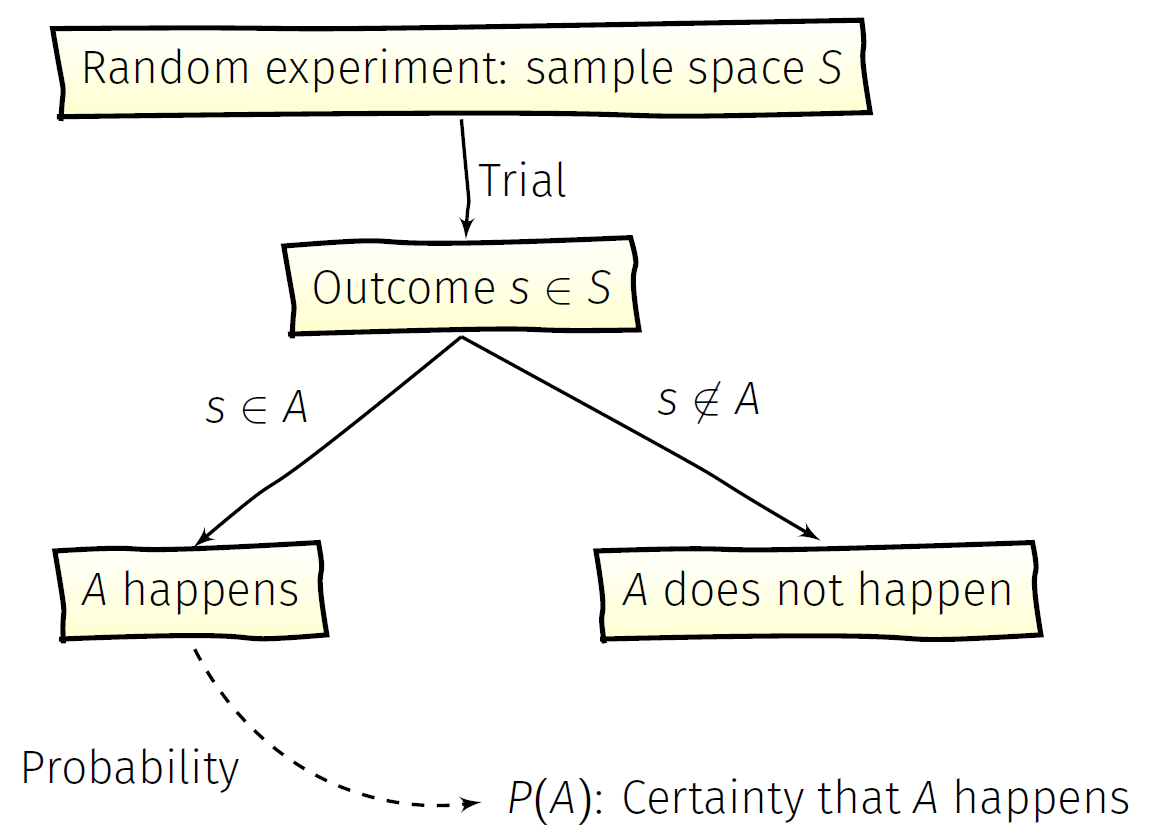
\includegraphics[width=0.65\textwidth]{figs/1_review_prob_intuition.PNG}
    \caption{Intuition of probability. Figure obtained from \cite{psaromiligkos_slides_2019}.}
    \label{fig:prob. intuition}
\end{figure}

\begin{mydefinition}[Probability]
    \emph{Probability} is a set function $\prob{}:\pSet_{S}\mapsto [0,1]$ that assigns to an event $A\in\pSet_{S}$ (recall $A\subseteq S)$ a number $\prob{A}$ that satisfies the following three axioms:
    \begin{enumerate}
        \item $\prob{A}\geq0$,
        \item $\prob{S}=1$, and
        \item For any sequence of mutually exclusive events $A_{1}, A_{2}, \ldots$ (i.e., for which $A_{i}\bigcap A_{j}=\emptyset$ for $i\neq j$), we have
        \begin{align}
            \prob{\bigcup_{i=1}^{\infty} A_{i}}=\sum_{i=1}^{\infty} \prob{A_{i}}.
        \end{align}
    \end{enumerate}
    The number $\prob{A}$ is called the probability of $A$.
\end{mydefinition}
\begin{remark}
        It is NOT always possible to define a function $P:\pSet\mapsto[0,1]$ that satisfies the three axioms.
        Workaround: focus on the events in a $\sigma$-algebra $\fCal$.
        
        Here are some other remarks about the probability function.
        \begin{myBlueBox}
            \begin{itemize}
                \item The probability function $\prob{}:\pSet_{S}\mapsto[0,1]$ maps  the power set $\pSet_{S}$ (or $\sigma$-algebra) to $[0,1]$. That is, the argument of $P$ should be an \emph{element} of $\pSet_{S}$. And since $\pSet_{S}$ is a \emph{set of sets} of $S$, then the argument is the event which is denoted by $\{a_{1},a_{2},\ldots,a_{n}\}=A\in\pSet_{S}$, where $a_{1}, \ldots, a_{n} \in S$.  Thus the proper way to write ``the probability of event $A$'' is $\prob{\{A\}}$ but the notation $\prob{A}$ will often be used for ease of reading and writing.

                \item Note that $\prob{A} = 0$ implies that event $A$ is \emph{improbable}; not necessarily impossible! It's still possible to get $A$. This might be a little unintuitive, but it can be thought of that the chance of $A$ happening is so small that it seems that event $A$ is highly unlikely to occur.
                \item Similarly, $\prob{A}= 1$ does NOT imply that $A$ will certainly occur! It just implies that it is very probably.
            \end{itemize}
        \end{myBlueBox}
\end{remark}

\begin{mydefinition}[$\sigma$-algebra]
    A set $\fCal$ of subsets of $S$, that is, $\fCal\subseteq \pSet$ is \emph{$\sigma$-algebra} if and only if
    \begin{enumerate}
        \item $S\in\fCal$,
        \item $E\in\fCal\implies E^{\comp}\in\fCal$, and
        \item If the sets $A_{1}, A_{2}, \ldots$ belong to $\fCal$, then so does $\bigcup_{i=1}^{\infty}A_{i}$.
    \end{enumerate}
    If $S$ is countable, then $\fCal=\pSet_{S}$ is used.
\end{mydefinition}
A random experiment is modeled as a probability space.
\begin{mydefinition}[Probability space]
    \label{def: proability space}
    A \emph{probability space} is a triplet
    \begin{align}
        (S, \fCal, \prob{}),
    \end{align}
    where
    \begin{enumerate}
        \item $S$: is the sample set,
        \item $\fCal$ is the events algebra, and
        \item $\prob{}:\fCal\mapsto[0,1]$ is the probability function.
    \end{enumerate}
\end{mydefinition}

\section{Basic theorems}
\begin{mytheoremarg}[Basic theorems]
    \label{thm:basic theorems of probability}
    Below is a list of basic theorems of probability.
    \begin{enumerate}
        \item For any event $A\in\fCal$, 
        \begin{align}
            \prob{A^{\comp}} = 1-\prob{A}.
        \end{align}

        \item For any event $A\in\fCal$, 
        \begin{align}
            0\leq \prob{A} \leq 1.
        \end{align} 
        
        \item $\prob{\emptyset} = 0$.
        \item For any events $A, B\in\fCal$, 
        \begin{align}
            \prob{A-B} = \prob{A} - \prob{A\cap B}.
        \end{align}
        Special case: if $B\subseteq A$, then
        \begin{align}
            \prob{A-B} = \prob{A}-\prob{B}.
        \end{align}
        
        \item For any $A, B \in \fCal$, 
        \begin{align}
            \prob{A} = \prob{AB} + \prob{AB^\comp}.
        \end{align}
        
        \item For any $A,B\in\fCal$,
        \begin{align}
            \prob{A\cap B} &= \prob{A} + \prob{B} - \prob{A\cup B},\\
            \prob{A\cup B} &= \prob{A} + \prob{B} - \prob{A\cap B}.
        \end{align}
    \end{enumerate}
\end{mytheoremarg}

\section{Conditional probabilities}
 Events can affect other events. Therefore, the question ``what's the probability of event $A$ happening?'' could be quite different from ``what's the probability of event $A$ \emph{given that event $B$ happened}?''\footnote{In some cases, the two questions are the same. This brings the notion of independence.}. The notation
 \begin{align}
   \prob{A |~ B}    
 \end{align}
reads ``probability of event $A$ happening given that event $B$ happened''.

Given 
\begin{enumerate}
    \item a random experiment $(S, \mc{F}, \prob )$, and
    \item $A, ~B\in\mc{F}$ with $\prob{B}\neq0$.
\end{enumerate}

\begin{mydefinition}
    [Conditional probability]    
    The conditional probability of $A$ given $B$, $\prob{A\middle|~B}$, defined as 
    \begin{align}
        \prob{A|B} &= \f{\prob{A\bigcap B}}{\prob{B}}.
    \end{align}    
\end{mydefinition}
\begin{mytheorem}
  [Conditional probability]    
  Let $B\in\mc{F}$ with $\prob{B}\neq 0$. The mapping 
  \begin{align}
    \prob{\cdot|B}:\mc{F}\to\rnums,
  \end{align}  
  satisfies the axioms of probability
  \begin{enumerate}
      \item $\prob{A|B}\geq 0,\quad \forall A\in\mc{F}$
      \item $\prob{S|B}=1$
      \item If $A_{1}, A_{2},\ldots\in\mc{F}$ is a sequence of mutually exclusive events, then
      \begin{align}
        \prob{\bigcup_{i=1}^{\infty}A_{i}|~B} &= \sum_{i=1}^{\infty}\prob{A_{i}|B}.
      \end{align}
  \end{enumerate}
\end{mytheorem}
Therefore,
\begin{itemize}
    \item For a given event $B$ with $\prob{B}\neq 0$, the mapping
    \begin{align}
        \prob{\cdot | B} : \mc{F}\to\rnums,
    \end{align}
    defines a valid probability function.
    \item All the basic theorems of probability listed in Theorem~\ref{thm:basic theorems of probability}apply to $\prob{\cdot|B}$.
\end{itemize}
\begin{myBlackBox}
    Here are some properties of conditional probability
    \begin{enumerate}
        \item For $A, B \in\mc{F}$ with $\prob{A},\prob{B}\neq0$:
        \begin{align}
            \prob{AB} &= \prob{A|B}\prob{B} \\
            &= \prob{B|A}\prob{A}.
        \end{align}

        
        \item \textbf{Total probability}. Let $B_{1},B_{2},\ldots,B_{n}$ be a partition of $S$, with $\prob{B_{i}}\neq 0,\forall i$:
        \begin{align}
            \prob{A} &= \prob{A|B_{1}}\prob{B_{1}} + \prob{A|B_{2}}\prob{B_{2}} + \ldots + \prob{A|B_{n}}\prob{B_{n}}\\
            &= \sum_{i=1}^{n}\prob{A|B_{i}}\prob{B_{i}}.
        \end{align}
        
        \item \textbf{Bayes rule}. Let $B_{1},B_{2},\ldots,B_{n}$ be a partition of $S$, with $\prob{B_{i}}\neq 0,\forall i$:
        \begin{align}
            \prob{B_{i}|A} &= \f{
                \prob{A|B_{i}}\prob{B_{i}}
            }{
                \sum_{j=1}^{n}\prob{A|B_{j}}\prob{B_{j}}
            }.            
        \end{align}
        Special case for $n=1$:
        \begin{align}
            \prob{B|A} &= \f{\prob{A|B}\prob{B}}{\prob{A}}.
        \end{align}
    \end{enumerate}
\end{myBlackBox}

\begin{mydefinition}
  [Indpendence]    
  \label{def:independence}
  The events $A, B\in\mc{F}$ are called \emph{independent} if 
  \begin{align}
    \underbrace{
      \prob{A|B}=\prob{A}}_{\text{requires } \prob{B}\neq0}
      \text{  or  }
    \underbrace{
        \prob{B|A}=\prob{B}}_{\text{requires } \prob{A}\neq0}
      \text{  or  }    
        \prob{AB}=\prob{A}\prob{B}
  \end{align}
\end{mydefinition}
\begin{mydefinition}
  [Independence (multiple events)]    
  The events $A, B, C\in\mc{F}$ are called \emph{independent} if
  \begin{itemize}
      \item They are independent in pairs, \underline{and}
      \item $\prob{ABC}=\prob{A}\prob{B}\prob{C}$.
  \end{itemize}
\end{mydefinition}
\begin{mydefinition}
  [Conditional independence]    
  Events $A, B\in\mc{F}$ are called \emph{conditionally independent given $C\in\mc{F}$, with $\prob{C}\neq 0$}, if
  \begin{align}
      \prob{AB|C} &= \prob{A|C}\prob{B|C}.
  \end{align}
\end{mydefinition}
\begin{myBlueBox}
    \textbf{Remark:} Conditional independence is quite different from independence. They do not imply each other. Here are some examples.
    
    \begin{example}[Independent but conditionally dependent]
        Two fair coins are flipped. Define the following events
        \begin{itemize}
            \item $A$ - Your first coin flip is heads,
            \item $B$ - Your second coin flip is heads, and
            \item $C$ - Your first two flips were the same.
        \end{itemize}
        Then $A$ and $B$ are independent. However, $A$ and $B$ are conditionally dependent given $C$, since if you know $C$ then your first coin flip will inform the other one.    
    \end{example}
    \begin{example}[Dependent but conditionally independent]
        Consider two brothers John and Joseph, both having a genetic disease. These two events are dependent as they are brothers. However, given the condition that Joseph is an adopted son of the family makes the events independent.
    \end{example}
\end{myBlueBox}

\section{Random variables and distributions}
In many random experiments, it is convenient to assign numerical labels to outcomes.
\begin{example}
    Experiment: pick a car out of a black Escort ($Eb$), a red Escort ($Er$), and a red Mazda ($Mr$).
    The sample space is then 
    \begin{align}
        S = \left\{ Eb, Er, Mr\right\},
    \end{align}
    and the events algebra is $\mc{F}=\pSet$.

    Say we are interested in the make of the car and not the color. Then we can assign labels as can be seen in Figure~\ref{fig:1 assigning numerical labels to outcomes}.
    \begin{figure}[h]
        \centering
        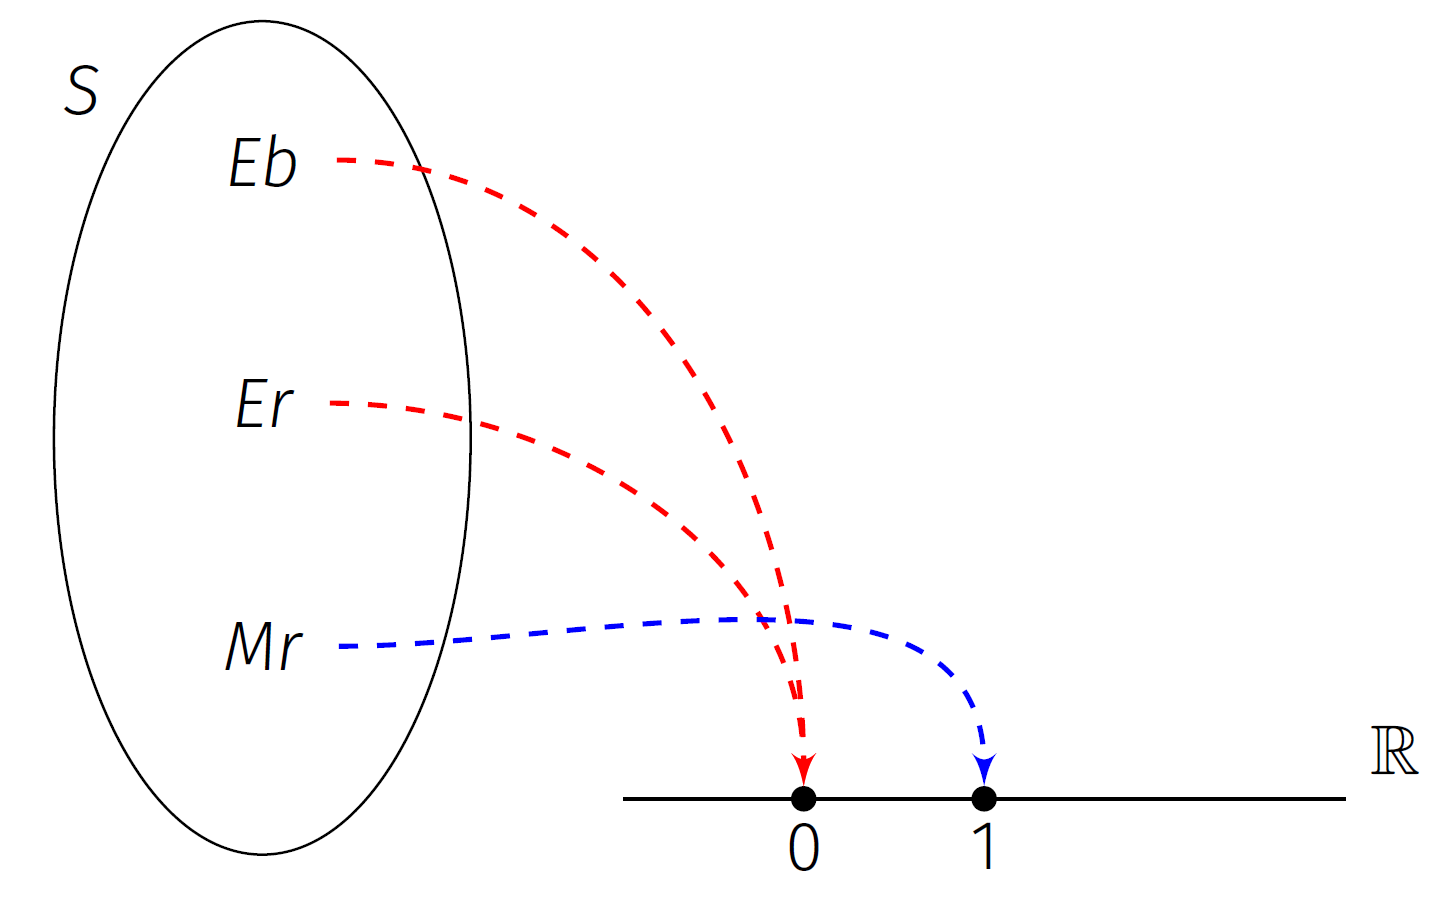
\includegraphics[width=0.65\textwidth]{figs/1_RV_example_labels_car.PNG}    
        \caption{Assigning numerical labels to outcomes; each color is an outcome. From~\cite{psaromiligkos_slides_2019}}
        \label{fig:1 assigning numerical labels to outcomes}
    \end{figure}
\end{example}
\begin{mydefinition}
  [Random variable (RV)]    
  A \emph{random variable (RV)} (denoted by an underline) $\rv{x}:S\to\rnums$ is a mapping from $S$ to $\rnums$ with the following properties.
  \begin{enumerate}
      \item $A(x) = \left\{ s\in S : \rv{x}(s)\leq x\right\}\in\mc{F}, \forall x\in\rnums$
      \item $\prob{\left\{ s\in S: \rv{x}(s)=\infty\right\}}=0$ and $\prob{\left\{ s\in S: \rv{x}(s)=-\infty\right\}}=0$
  \end{enumerate}
  $S$ is referred to as the \emph{domain} of the RV $\rv{x}(\cdot)$ (since a RV is a mapping, then it has a domain and a range). [The domain can be thought of as the sample space\footnote{Not quite sure of this statement.}.]
\end{mydefinition}
\begin{mydefinition}
  [Cumulative distribution function (CDF)]    
  The function $F : \rnums\to[0,1]$ defined by 
  \begin{align}
      F(x) 
      \label{eq:def CDF full}
      &= \prob{s\in S : \rv{x}(s)\leq x}\\
      \label{eq:def CDF shorthand}
      &= \prob{\rv{x}\leq x}, \quad \forall x\in\rnums
  \end{align}
  is called the \emph{cumulative distribution function (CDF)} of $\rv{x}$. Note that \eqref{eq:def CDF shorthand} is a shorthand for \eqref{eq:def CDF full}.

  \textbf{Note:} sometimes the CDF will be denoted with a subscript of the RV (e.g., $F_{x}(x)$). This is for clarity as to make sure that the CDF is over the RV $\rv{x}$. This come more in handy when there are multiple variables in hands (such as in integration).
\end{mydefinition}

\subsection{Properties of random variables}
Here are some properties of random variables.
\begin{enumerate}
    \item $\lim_{x\to\infty} F_{x}(x) =1$ and $\lim_{x\to-\infty} F_{x}(x)=0$
    \item $F_{x}(x)$ is non-decreasing 
    \item $F_{x}(x)$ is continuous from the right. That is
    \begin{align}
        \lim_{x\to x_{0}^{+}} F_{x}(x) &= F_{x}(x_{0})
    \end{align}
    \item $\prob{\left\{ x_{1}<\rv{x}\leq x_{2}\right\}}=F_{x}(x_{2})-F_{x}(x_{1})$
    \item $\prob{\left\{ \rv{x}=x_{1}\right\}}=F_{x}(x_{1})-F_{x}(x_{1}^{-})$, where $F_{x}(x_{1}^{-}):=\lim_{x\to x_{1}^{-}} F_{x}(x)$
    \item $\prob{\left\{ x_{1}\leq \rv{x} \leq x_{2}\right\}}=F_{x}(x_{2})-F_{x}(x_{1}^{-})$
\end{enumerate}

\begin{mydefinition}
  [Types of RVs]    
  A RV $\rv{x}$ is called 
  \begin{itemize}
      \item \emph{Discrete} if $F_{x}(x)$ is constant except of countable number of discontinuities (piecewise constant). Figure~\ref{fig: example CDF discrete RV} shows an example of a CDF of a discrete RV.
      \item \emph{Continuous} if $F_{x}(x)$ is
      \begin{enumerate}
          \item continuous, and
          \item differentiable (with the exception of a countable number of point).
      \end{enumerate}
      \item \emph{Mixed} if it is neither continuous nor discrete.
  \end{itemize}
\end{mydefinition}

\begin{mydefinition}
  [Probability mass function (PMF)]    
  Let $\rv{x}$ be a discrete RV. Then,
  \begin{itemize}
      \item $\prob{\rv{x}=x}=0$ when $x\neq x_{i}, i=1,2,\ldots$, 
      \item $\mc{R}_{x}=\left\{ x_{i} : i=1,,2,\ldots\right\}$ is the set of possible points. 
  \end{itemize}

  The \emph{probability mass function (PMF)} of a RV $\rv{x}$, $\pmf{x}$ or $p_{x}(x)$, $x\in\rnums$, is defined as 
  \begin{align}
      \pmf{x} &= \prob{\rv{x}=x} &= 
      \begin{cases}
          0 & \text{if } x\notin \mc{R}_{x},\\
          \prob{\rv{x}=x_{i}} & \text{if } x\in\mc{R}_{x}, \text{ i.e., } x=x_{i}, i=1,2,\ldots.
      \end{cases}
  \end{align}
  Also,
  \begin{itemize}
      \item $\sum_{i=1}^{\infty}\pmf{x_{i}} = 1$ and $\pmf{x}\geq 0$, $\forall x$ (defining properties),
      \item $\prob{\rv{x}\in \mc{A}}=\sum_{x_{i}\in \mc{A}} \pmf{x_{i}}$.
  \end{itemize}
\end{mydefinition}

\begin{figure}[h]
    \centering
    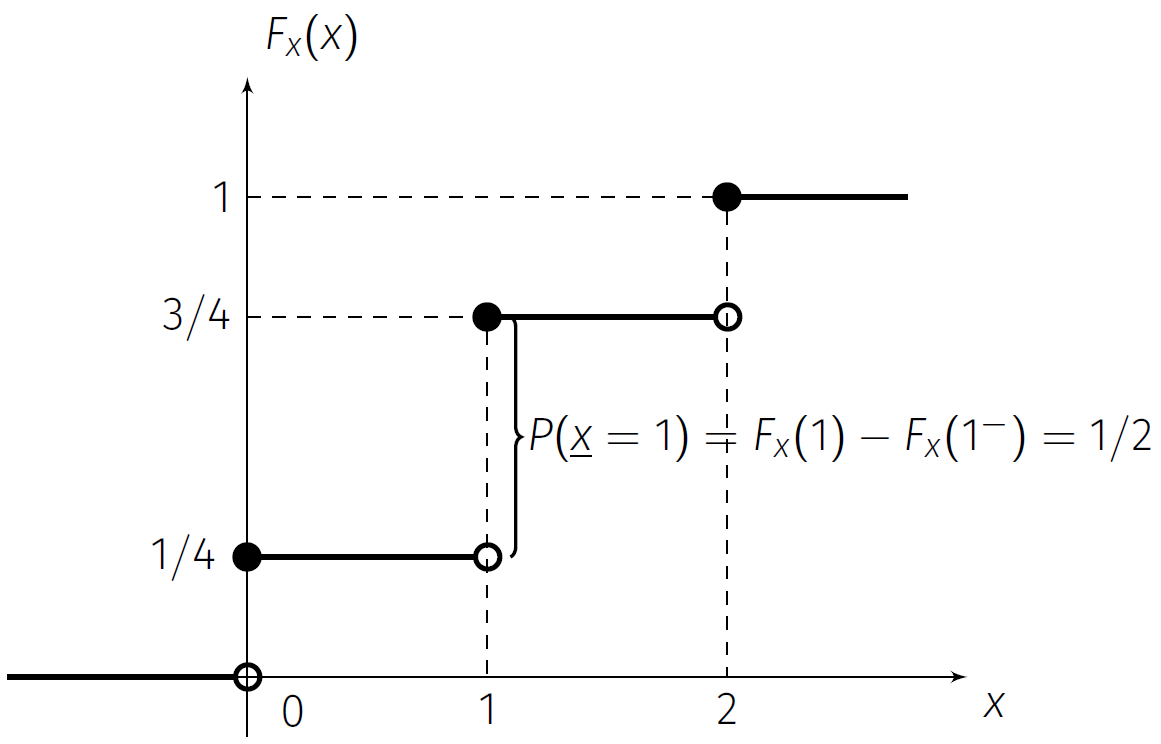
\includegraphics[width=0.65\textwidth]{figs/1_RV_example_discrete.PNG}    
    \caption{Example of a CDF of a discrete RV. From~\cite{psaromiligkos_slides_2019}.}
    \label{fig: example CDF discrete RV}
\end{figure}

\begin{mydefinition}
  [Porbability density function (PDF)]    
  The \emph{probability density function (PDF)}, $\pdf{x}$ or $\pdf{}_{x}(x)$, of a RV $\rv{x}$ is defined as
  \begin{align}
      \pdf{}_{x}(x) &= \td{\cdf{}_{x}(x)}{x}.
  \end{align}
\end{mydefinition}

\subsection{Properties of PDFs}
If $\rv{x}$ is continuous with PDF $\pdf{x}$
\begin{enumerate}
    \item $\pdf{}_{x}(\rv{x})\geq 0, \forall x$ (defining property)
    \item $\int_{-\infty}^{x}\pdf{}_{x}(\lambda)\dee\lambda = \cdf{}_{x}(x)$
    \item $\int_{-\infty}^{\infty}\pdf{}_{x}(x)\dee\lambda = 1$ (defining property)
    \item 
    \begin{align}
        \prob{\left\{ a\leq \rv{x}\leq b\right\}} &= \int_{a}^{b}\pdf{}_{x}(\lambda)\dee\lambda \\
        \prob{\left\{ a< \rv{x}\leq b\right\}} &= \prob{\left\{ a\leq \rv{x}< b\right\}} = \prob{\left\{ a< \rv{x}< b\right\}}.
    \end{align}
\end{enumerate}
\begin{myBlackBox}
    \textbf{Interpretation of PDF}: For a continuous $\rv{x}$: $\prob{\rv{x}=x}=0$ for all $x\in\rnums$ which implies that the PDF $\pdf{x}$ is \emph{not} a probability.

    For small $\epsilon>0$: 
    \begin{align}
        \prob{\abs{\rv{x}-x}<\epsilon} &= \prob{x-\epsilon<\rv{x}<x+\epsilon}\\
        &= \int_{x-\epsilon}^{x+\epsilon}\pdf{t}\dee t\\
        &\approx 2\epsilon\pdf{x}
    \end{align}
    assuming $\pdf{x}$ is continuous at $x$. Equivalently,
    \begin{align}
        \pdf{x}&\approx \f{1}{2\epsilon}\prob{x-\epsilon<\rv{x}<x+\epsilon}.
    \end{align}
    $\pdf{x}$ is proportional to the probability that $\rv{x}$ lies in a small neighbourhood of $x$.
\end{myBlackBox}


\subsection{Conditional distributions}
\begin{mydefinition}[Conditional distributions]      
    \label{def:SRV conitional distributions}
    Let $M\in\mc{F}$ with $\prob{M}\neq 0$. Then
    \begin{enumerate}
        \item \emph{Conditional CDF} of $\rv{x}$ given event $M$ is 
        \begin{align}
            \cdf{}_{x}(x|M) &= \prob{\rv{x}\leq x|M}\\
            &= \f{\prob{\rv{x}\leq x,M}}{\prob{M}}.
        \end{align}
        \item \emph{Conditional PDF} of $\rv{x}$ given event $M$ is
        \begin{align}
            \pdf{}_{x}(x|M) &= \td{\cdf{}_{x}(x|M)}{x}.
        \end{align}
        \item \emph{Conditional PMF} of $\rv{x}$ ($\rv{x}$ discrete given $M$) is
        \begin{align}
            \pmf{x|M} 
            &=
            \begin{cases}
                0, &x \notin\left\{ x_{i} : i = 1,2,\ldots\right\}\\
                \prob{\rv{x}=x_{i}|M}, &x\in\left\{ x_{i} : i=1,2,\ldots\right\}.
            \end{cases}
        \end{align}
        Note that conditional CDFs, PDFs, and PMFs behave like unconditional ones.
    \end{enumerate}
\end{mydefinition}
\subsubsection*{Properties of conditional distributions}
Let $B_{1}, B_{2}, \ldots, B_{n}$ be a partition of $S$, $\prob{B_{i}}\neq 0$. Let $A\in\mc{F}$, $\prob{A}\neq0$.
\begin{itemize}
    \item \textbf{Total probability}:
    \begin{align}
        \cdf{}_{x}(x) &= \sum_{i=1}^{n} \cdf{}_{x}(x|B_{i})\prob{B_{i}},\\
        \pdf{}_{x}(x) &= \sum_{i=1}^{n} \pdf{}_{x}(x|B_{i})\prob{B_{i}},\\
        \pmf{}_{x}(x) &= \sum_{i=1}^{n} \pmf{}_{x}(x|B_{i})\prob{B_{i}}.
    \end{align}
    \item \textbf{Bayes rule}: 
    \begin{align}
        \prob{A|\rv{x}\leq x} 
        &= \f{\prob{\rv{x}\leq x, A}}{\prob{\rv{x}\leq x}}\\
        &= \f{\prob{\rv{x}\leq x|A}\prob{A}}{\prob{\rv{x}\leq x}}\\
        &= \f{\cdf{}_{x}(\rv{x}\leq x|A)\prob{A}}{\cdf{}_{x}({\rv{x}\leq x})}.
    \end{align}
\end{itemize}
When $\rv{x}$ is discrete with $\mc{R}_{x}=\left\{ x_{1},x_{2},\ldots\right\}$, $\pmf{x_{i}}\neq0$:
\begin{itemize}
    \item \textbf{Conditional probability} using PMF:
    \begin{align}
        \prob{A|\rv{x}=x_{i}} 
        &= \f{\prob{A,\rv{x}=x_{i}}}{\prob{\rv{x}=x_{i}}}\\
        &= \f{\prob{A,\rv{x}=x_{i}}}{\pmf{}_{x}({\rv{x}=x_{i}})}.
    \end{align}
    \item \textbf{Total probability}:
    \begin{align}
        \prob{A} &= \sum_{i=1}^{\infty}\prob{A|\rv{x}=x_{i}}\pmf{x_{i}}.
    \end{align}
    \item \textbf{Bayes rule}:
    \begin{align}
        \pmf{x|A} 
        &= \f{\prob{A|\rv{x}=x}\pmf{x}}{\prob{A}}\\
        &= \f{\prob{A|\rv{x}=x}\pmf{x}}{\sum_{i=1}^{\infty}\prob{A|\rv{x}=x_{i}}\prob{x_{i}}}.
    \end{align}
\end{itemize}
When $\rv{x}$ is continuous, it is not possible to divide by $\prob{\rv{x}=x}=0$. Therefore, another definition for conditional PDF is needed.
\begin{mydefinition}
  [Conditional PDF]    
  The \emph{conditional PDF} of $A\in\mc{F}$ given $\rv{x}=x$ (assuming $\pdf{}_{x}(x)\neq0$) is
  \begin{align}
      \prob{A| \rv{x}=x} &= \f{\pdf{}_{x}(x|A)\prob{A}}{\pdf{}_{x}(x)}.
  \end{align}
\end{mydefinition}
The properties of such conditional PDF are
\begin{itemize}
    \item \textbf{Total probability}: $\prob{A}=\int_{-\infty}^{\infty} \prob{A|\rv{x}=x}\pdf{}_{x}(x)\dee x$/
    \item \textbf{Bayes rule}:
    \begin{align}
        \pdf{}_{x}(x|A) 
        &= \f{\prob{A|\rv{x}=x}\pdf{}_{x}(x)}{\prob{A}}\\
        &= \f{\prob{A|\rv{x}=x}\pdf{}_{x}(x)}{\int_{-\infty}^{\infty}\prob{A|\rv{x}=x}\pdf{}_{x}(x)\dee x}.
    \end{align}
\end{itemize}



\section{Transformed random variables}
\label{sec: SRV: Transformed random variables}
Say there exists a random variable $\rv{x}: S\to\rnums$ that is applied on the probability space $(S,\mc{F},\prob{})$. Further, say there exists a [deterministic] function $g:\rnums\to\rnums$. Then, there is a new RV $\rv{y}$ defined as 
\begin{align}
    \rv{y}(s) &= g(\rv{x}(s)) \quad\forall s\in S.
\end{align}
Furthermore, say the distribution (i.e., CDF and PDF (or PMF)) of $\rv{x}$ is known. THen what is the distribution of $\rv{y}=g(\rv{x})$?

The foundation is the following
\begin{align}
    \prob{\rv{y}\in{A}}
    &= \prob{\left\{ s\in S : \rv{y}(s)\in A\right\}}\\
    &= \prob{\left\{ s\in S : g(\rv{x}(s))\in A\right\}}.
\end{align}

There are different methods to find the distribution of a transformed random variable (i.e., $\rv{y}=g(\rv{x})$) depending on the types of variables.
\begin{enumerate}
    \item \textbf{Method of distributions} works when for \emph{any} types of random variables (continuous or discrete). However, it is the most exhaustive method.
    \item \textbf{Method of transformations} works for \emph{continuous} random variables; i.e., both $\rv{x}$ and $\rv{y}$ are continuous.
    \item \textbf{Discrete transformation} for \emph{discrete} transformed variable $\rv{y}$ and \emph{continuous} or \emph{discrete} domain random variable $\rv{x}$.
\end{enumerate}

\subsection{Method of distribution}
The method will be motivated by an example. 
\begin{example}
    Consider the transformed random variable
    \begin{align}
        \rv{y} 
        &= g(\rv{x})\\
        &= \rv{x}^{2}.
    \end{align}
    Evaluate the CDF as follows
    \begin{align}
        \cdf{}_{y}(y) &= \prob{\rv{y}\leq y} = \prob{g(\rv{x})\leq y} = \prob{\rv{x}^2\leq y}\\
        &= \prob{\left\{ s\in S : \rv{x}(s)^{2}\leq y\right\}}.
    \end{align}
    There are three cases
    \begin{enumerate}
        \item $y<0$: $\prob{\rv{x}^{2}\leq y} = 0 \implies \cdf{}_{y}(y) = 0$.
        \item $y=0$: $\prob{\rv{x}^{2}\leq 0} = \prob{\rv{x}^{2}=0} = \prob{\rv{x}=0} \implies \cdf{}_{y}(0)=\prob{\rv{x}=0}$.
        \item $y>0$: $\prob{\rv{x}^{2}\leq y} = \prob{\abs{\rv{x}}\leq \sqrt{y}} = \prob{-\sqrt{y}\leq \rv{x} \leq\sqrt{y}}\implies$
        \begin{align}
            \cdf{}_{y}(y) &= \int_{-\sqrt{y}}^{\sqrt{y}} \pdf{}_{x}(x)\dee x.            
    \end{align}
    \end{enumerate}
\end{example}

\subsection{Method of transformation}
The process is outlined by the following steps. 

\begin{myBlackBox}
    For any $y$ (treat it as a deterministic variable):
    \begin{enumerate}
        \item Solve $g(x)=y$ for $x$. List \emph{all} possible solutions $x_{1},x_{2},\ldots,x_{n}$.
        \item Calculate $g'(x) = \td{g(x)}{x}$.
        \item Evaluate 
        \begin{align}
            \pdf{}_{y}(y) 
            &= 
            \begin{cases}
                0, &\text{no solutions to }g(x)=y,\\
                \sum_{i=1}^{n} \f{\pdf{}_{x}(x_{i})}{\abs{g'(x_{i})}}, &\text{otherwise}.
            \end{cases}
        \end{align}
    \end{enumerate}
\end{myBlackBox}
The method is derived in \cite[Sec.~2.6.2]{murphy_machine_2012}. 

\begin{example}[Method of transformation]
    Consider 
    \begin{align}
        \rv{y} 
        &= g(\rv{x})\\
        &= \rv{x}^{2}.
    \end{align}
    Carry the steps:
    \begin{enumerate}
        \item Solve for $x$ in $y=g(x)$ for all possible cases of $y$:
        \begin{enumerate}
            \item $y<0$: No solutions.
            \item $y=0$: One solution $x_{1}=0$.
            \item $y>0$: Two solutions $x_{1}=-\sqrt{y}$ and $x_{2}=\sqrt{y}$.
        \end{enumerate}
        \item Calculate the derivative of the function
        \begin{align}
            g'(x) &= 2x, \quad \forall x.
        \end{align}
        \item Calculate $\pdf{}_{y}(y)$:
        \begin{enumerate}
            \item $y<0$: $\pdf{}_{y}(y) = 0$.
            \item $y=0$: $\pdf{}_{y}(0)=0$.            
            \item $y>0$: 
            \begin{align}
                \pdf{}_{y}(y) &= \f{\pdf{}_{x}(-\sqrt{y})}{\abs{-2\sqrt{y}}} + \f{\pdf{}_{x}(\sqrt{y})}{\abs{2\sqrt{y}}}\\
                &= \f{1}{2\sqrt{y}}\left[ \pdf{}_{x}(-\sqrt{y}) + \pdf{}_{x}(\sqrt{y}) \right].
            \end{align}
        \end{enumerate}
    \end{enumerate}
    \triqed
\end{example}


\subsection{Discrete transformation}
The method will be motivated by two examples:
\begin{enumerate}
    \item continuous to discrete transformation, and
    \item discrete to discrete transformation.
\end{enumerate}
\begin{example}[Continuous to discrete transformation]
    Let $\rv{x}$ be continuous with $f(x)=0$, $x<0$ and
    \begin{align}
        \rv{y} &= g(\rv{x})\\
        &= \floor{\rv{x}} \quad \text{(floor of $\rv{x}$)}.
    \end{align}
    Then the transformed variable $\rv{y}$ is discrete. I.e., $\mc{R}_{y}=\left\{ 0,1,2,\ldots\right\}$.
    
    The PMF of $\rv{y}$ is then given by 
    \begin{align}
        \pmf{}_{y}(y) 
        &= \prob{\rv{y}=y}\\
        &= \prob{\floor{\rv{x}}=y}\\
        &= \prob{y\leq \rv{x}<y+1}\\
        &= \int_{y}^{y+1}\pdf{}_{x}(x)\dee x, \quad y = 0,1,2,\ldots.
    \end{align}
    \triqed
\end{example}
\begin{example}[Discrete to discrete transformation]
    Let $\rv{x}$ be discrete with $\mc{R}_{x}=\mbb{Z}$, and 
    \begin{align}
        \rv{y}
        &= g(\rv{x})\\
        &= \abs{\rv{x}}.
    \end{align}
    Then $\rv{y}$ is also discrete random variable with $\mc{R}_{y}=\left\{ 0,1,2,\ldots\right\}$.

    The PMF of $\rv{y}$ can then be given by
    \begin{align}
        \pmf{}_{y}(y) &= \prob{\rv{y}=y}\\
        &= \prob{\abs{\rv{x}}=y}\\
        &= \prob{\rv{x}=\pm y}\\
        &= 
        \begin{cases}
            \pmf{}_{x}(0), & y=0,\\
            \pmf{}_{x}(-y)+\pmf{}_{x}(y), & y=1,2,\ldots.
        \end{cases}
    \end{align}
    \triqed
\end{example}

\section{Statistics of random variables}
Sometimes, information about the random variables such as the mean is sought after. Information about a random variables are referred to as the \emph{statistics} of it.
\begin{mydefinition}
  [Expectation operator]    
  \label{def: SRV expectation operator}
  The expectation operator $\expect{\cdot}$ is a functional operator that operates on random variables. Specifically:
  \begin{itemize}
      \item For continuous random variables
      \begin{align}
          \expect{g(\rv{x})}
          &= \int_{-\infty}^{\infty} g(x)\pdf{x}\dee x.
        \end{align}
        \item For discrete random variables 
        \begin{align}
            \expect{g(\rv{x})}
            &= \sum_{-\infty}^{\infty} g(x)\pmf{x}.
        \end{align}
  \end{itemize}
  
\end{mydefinition}

\begin{mydefinition}
  [Mean of a random variable]    
  The mean of a random variable $\rv{x}$, $\mu_{x}$, is defined as
  \begin{align}
      \mu_{x} &= \expect{\rv{x}}      
  \end{align}
  which 
  \begin{itemize}
      \item for continuous random variable 
      \begin{align}
        \mu_{x} &= \expect{\rv{x}}\\
        &= \int_{-\infty}^{\infty}x\pdf{x}\dee x,
      \end{align}
      \item while for discrete random variable
      \begin{align}
        \mu_{x} &= \expect{\rv{x}}\\
        &= \sum_{-\infty}^{\infty}x\pmf{x}.
      \end{align}
  \end{itemize}
  and the conditional mean of $\rv{x}$ given event $M$ is
  \begin{align}
      \expect{\rv{x}|M} &= \int_{-\infty}^{\infty} x\pdf{x|M}\dee x.
  \end{align}
\end{mydefinition}

\subsection*{Properties of the mean}
\begin{itemize}
    \item Mean of $\rv{y}=g(\rv{x})$ is
    \begin{align}
        \expect{\rv{y}} &= \expect{g(\rv{x})}\\
        &= \int_{-\infty}^{\infty}g(x)\pdf{}_{x}(x)\dee x.
    \end{align}
    \item Linear property:
    \begin{align}
        \expect{\sum_{i=1}^{n}\alpha_{i}g_{i}(\rv{x})} &= \sum_{i=1}^{n}\alpha_{i}\expect{g_{i}(\rv{x})}.
    \end{align}
    Note that in general,
    \begin{align}
        \expect{g(\rv{x})} \neq g(\expect{\rv{x}}).
    \end{align}
\end{itemize}

\begin{mydefinition}
  [Variance and standard deviation]    
  Let $\rv{x}$ be a random variable. Then the \emph{variance} of $\rv{x}$, $\var{\rv{x}}$, is defined as
  \begin{align}
      \var{\rv{x}} &= \sigma_{x}^{2}\\
      &= \expect{\left(\rv{x}-\expect{\rv{x}}\right)^2}\\
      &= \expect{\rv{x}^2} - \expect{\rv{x}}^2.
  \end{align}
  The \emph{standard deviation} of $\rv{x}$ is $\sigma_{x} = \sqrt{\var{\rv{x}}}$.

  A useful property of the variance is
  \begin{align}
      \var{a\rv{x}+b} &= a^2\var{\rv{x}}.
  \end{align}
\end{mydefinition}

\begin{mytheorem}[Markov's inequality]
    Let $\rv{x}$ be a non-negative random variable. That is, $\prob{\rv{x}<0}=0$. For any $\epsilon>0$:
    \begin{align}
        \prob{\rv{x}\geq \epsilon} \leq \f{\expect{\rv{x}}}{\epsilon}.
    \end{align}
\end{mytheorem}

\begin{mytheorem}[Chebyshev's inequality]
    Let $\rv{x}$ be a random variable with mean $\mu$ and variance $\sigma^2$. Then, for any $\epsilon>0$:
    \begin{align}
        \prob{\abs{\rv{x}-\mu}\geq \epsilon} \leq \f{\sigma^2}{\epsilon}.
    \end{align}
\end{mytheorem}

\begin{mytheorem}[Jensen's inequality]
    Let $g(\cdot)$ be a convex function. Then, 
    \begin{align}
        \expect{g(\rv{x})} \geq g(\expect{\rv{x}}).
    \end{align}
\end{mytheorem}

\subsection{Moments}

\begin{mydefinition}[Moments] 
    \label{def:moments single rv}
    The different moments of a random variable are defined as follows.   
    \begin{itemize}
        \item \emph{$n$-th moment} of $\rv{x}$: $m_{n}=\expect{\rv{x}^{n}}$.
        \item \emph{$n$-th central moment} of $\rv{x}$: $\mu_{n}=\expect{(\rv{x}-\expect{\rv{x}})^{n}}$.
        \item \emph{$n$-th absolute moment} of $\rv{x}$: $\expect{\abs{\rv{x}}^{n}}$.
        \item \emph{$n$-th absolute central moment} of $\rv{x}$: $\mu_{n}=\expect{\abs{\rv{x}-\expect{\rv{x}}}^{n}}$.
    \end{itemize}
\end{mydefinition}

\subsection{Characteristic functions}
\begin{mydefinition}
  [Characteristic function]    
  The \emph{characteristic function} of a random variable $\rv{x}$ is the Fourier transform of its PDF. Specifically,
  \begin{align}
      \Phi_{x}(\omega) &= \int_{-\infty}^{\infty} e^{\jmath \omega x}\pdf{}_{x}(x)\dee x,
  \end{align}
  where the inverse expression is given by
  \begin{align}
      \pdf{}_{x}(x) &= \f{1}{2\pi}\int_{-\infty}^{\infty} e^{-\jmath\omega x}\Phi_{x}(\omega) \dee \omega.
  \end{align}
\end{mydefinition}
\begin{mydefinition}
  [Moment generating function]    
  The \emph{moment generating function} of $\rv{x}$ is the Laplace transform of its PDF. Specifically, 
  \begin{align}
      \bar{\Phi}_{x}(s) &= \int_{-\infty}^{\infty} e^{Sx}\pdf{}_{x}(x)\dee x.
  \end{align}
\end{mydefinition}

\begin{mytheorem}[Moment theorem]
    \begin{align}
        \expect{\rv{x}^{n}} &= \left.\f{\dee^{n}}{\dee s^{n}}\bar{\Phi}_{x}\right|_{s=0} 
        = \left.\f{1}{\jmath^{n}}\f{\dee ^{n}}{\dee\omega^{n}}\Phi_{x}(\omega)\right|_{\omega=0}.
    \end{align}
\end{mytheorem}
% \clearpage
% \clearpage
% %%%%%%%%%%%%%%%%%%
% %%%%%%%%%%%%%%%%%%
% %%%%%%%%%%%%%%%%%%
% %   Old Notes
% %%%%%%%%%%%%%%%%%%
% %%%%%%%%%%%%%%%%%%

% \begin{itemize}
%     \item Definitions in slides.
%     \item Probability of an \textit{event}.
%     \item Event: 1,2,3,...,10 (even number could be an event).
%     \item Power set could. \eg, ((H,T),(H),(T),null-set).
%     \item Understand the definition of the event before interpreting the number/probability.
%     \item 
% \end{itemize}

% \begin{itemize}
%     % \item Probability is a measure of an \textit{outcome} ! Not an event!
    
%     \item Note that $P(A) = 0$ implies that event $A$ is \textit{improbable} and NOT impossible! It's still possible to get $A$. This might be a little unintuitive, but it can be thought of that the chance of $A$ happening is so small that it seems that it is highly unlikely to happen.
%     \item Similarly, $P(A) = 1$ does NOT imply that $A$ will occur! It just implies that it is very probably.
    
%     \item A random experiment is modelled as a probability space.
% \end{itemize}


% \subsection{Definitions}
% \begin{itemize}
%     \item A \textbf{probability} is a measure of our certainty or belief that a statement is true. Another definition is ``a probability is how frequently an event will occur''.
    
%     \item A \textbf{random experiment} is an experiment (or physical process) whose outcome is not certain but all of its \textit{possible} outcomes are known and predictable in advance.
    
%     \item The \textbf{sample space} $S$ is the set of all possible outcomes.
    
%     \item The \textbf{event} $A$ is a subset of $S$.
    
%     \item The \textbf{power set} of $S$ is the set containing all subsets of a set $S$.
%     \begin{itemize}
%         \item Notation: $\pSet_S$ or simply $\pSet$.
%         \item $\pSet$ : Set of all events.
%         \item Special events:
%         \begin{itemize}
%             \item $\emptyset \subseteq S$: Impossible event. ($\emptyset$ is the empty set.)
%             \item $S \subseteq S$: Certain event.
%         \end{itemize}
%     \end{itemize}
    
%     \item \textbf{Probability} is a \textit{set function} $P(\cdot)$ ($P:\pSet_{{S}}\mapsto\mathbb{R}$) that assigns an event $A\subseteq S$ a number $P(A)$ that satisfies the following three axioms:
%     \begin{enumerate}
%         \item $P(A) \geq 0$;
%         \item $P(S) = 1$;
%         \item For any sequence of mutually exclusive events $A_1, A_2, \dots$ (\ie, for which $A_i\cap A_j=\emptyset$ if $i\neq j$), then we have $$ P\left(\bigcap_{i=1}^{\infty}A_i\right) = \sum_{i=1}^{\infty}P(A_i).$$
%     \end{enumerate}
    
%     The number $P(A)$ is called the probability of $A$.
    
%     Remarks:
%     \begin{itemize}
%         \item We cannot \textit{always} define a function $P(\cdot)$ that satisfies the 3 axioms.
%         \item Workaround: focus on the events in a $\sigma-$algebra $\fCal$.
%     \end{itemize}
    
%     \item A set $\fCal$ of subsets of $S$ (\ie, $\fCal\subseteq\pSet_S$) is \textit{$\sigma-$algebra} if and only if 
%     \begin{enumerate}
%         \item $S\in\fCal$,
%         \item $E\in\fCal\implies E^{\comp}\in\fCal$, and
%         \item if the sets $A_i\in\fCal~\forall i\in\mathbb{N}_{+} \implies \bigcup_{i=1}^{\infty}A_i \in \fCal$.
%     \end{enumerate}
    
%     If $S$ is countable, then $\fCal = \pSet_S$ is used.
    
%     \item A \textbf{probability}
%     \footnote{Another definition based off $\sigma-$algebra.}
%     is a set function $P\colon\fCal\mapsto\mathbb{R}$ that assigns to an event $A\in\fCal$ a number $P(A)$ that satisfies the following three axioms:
%     \begin{enumerate}
%         \item $P(A) \geq 0$;
%         \item $P(S) = 1$;
%         \item For any sequence of mutually exclusive events $A_i\in\fCal~\forall i\in\mathbb{N}_{+}$ (\ie, for which $A_i\cap A_j=\emptyset$ if $i\neq j$), then we have $$ P\left(\bigcap_{i=1}^{\infty}A_i\right) = \sum_{i=1}^{\infty}P(A_i).$$
%     \end{enumerate}
    
%     The number $P(A)$ is called the probability of $A$.
    
%     \item A \textbf{probability space} is a triplet $\left(S, \fCal, \pSet\right)$.  Where $S$ is the sample space, $\fCal$ is the events algebra, and $P\colon\fCal\mapsto\mathcal{R}$ is the probability function.
% \end{itemize}


% \subsection{Theorems}
% \begin{enumerate}
%     \item $P(A) = 1-P(A^{\comp})$.
%     \item $0\leq P(A) \leq 1$.
%     \item $P(\emptyset) = 0$.
%     \item $P(A-B) = P(A) - P(A\cap B)$. Special case, if $B\subseteq A$, then $P(A-B) = P(A)-P(B)$.
    
%     \item For any $A, B \in \pCal$, $P(A) = P(AB) + P(AB^\comp)$.
    
%     \item For any $A,B\in\fCal$,
%     \begin{itemize}
%         \item $P(A\cap B)  = P(A) + P(B) - P(A\cup B)$, and 
%         \item $P(A\cup B) = P(A) + P(B) - P(A\cap B)$.
%     \end{itemize}
% \end{enumerate}

% %%%%%%%%%%%%%%%%%%%%%%%%%%%%%%%%%%%%




% \clearpage
% \section{Properties}
% Given a random experiment: $(S,\fCal, P)$. Then the conditional probability of event $A$ happening given that event $B$ happened is formally written as $P(A|B)$ and assuming $P(B) \neq 0$, $P(A|B)$ is given by
% \begin{equation*}
%     P(A|B) = \frac{P(A\cap B)}{P(B)}.
% \end{equation*}

% A useful form for $P(A) \neq 0$ and $P(B) \neq 0$ is 

% Useful properties
% \begin{itemize}
%     \item 
%     \begin{equation}
%         P(AB) = P(A|B)P(B) = P(B|A)P(A).    
%     \end{equation}
    
%     \item \textbf{Total probability}:
%     Let $B_1, B_2, ...$ be a partition\footnote{A set of grouping that sets \textbf{elements} into non-empty \textbf{subsets} in such a way that every element is matched in exactly one set.} of $S$ with $P(B_i) \neq 0~i=1,\dots,n$, then 
    
%     \begin{enumerate}
%         \item $P(A) = \sum_{i=1}^{n}P(A|B_i)P(B_i)$.
%         \item $$P(B_i|A) = \frac{P(A|B_i)P(B_i)}{\sum_{i=1}^{n}P(A|B_i)P(B_i)}.$$
%     \end{enumerate}
    
% \end{itemize}

% \subsection{Independence}
% Events $A,B \in \pCal$ are two independent events if 
% \begin{enumerate}
%     \item $P(AB) = P(A)P(B)$.
%     \item If $P(B) \neq 0$, $P(A|B) = P(A)$.
%     \item If $P(A) \neq 0$, $P(B|A) = P(B)$.
% \end{enumerate}

% Events $A, B, C \in \fCal$ are independent if 
% \begin{enumerate}
%     \item they're independent in pairs, and
%     \item $P(ABC) = P(A)P(B)P(C)$.
% \end{enumerate}


% %%%%%%%%%%%%%
% \section{Random variables}
% \subsection{Definition}
% A random variable $\underline{x}$ is basically a mapping from events to numbers (assigning numerical labels to outcomes). In mathematical terms, $\underline{x} : S \mapsto \mathbb{R}$ such that
% \begin{enumerate}
%     \item $A(x) = \{s\in S : \underline{x}(s) \neq x\} \in \fCal,~\forall x\in\mathbb{R}$. I.e., all possible outcomes $s\in S$ such that $\underline{x}(s)\leq x \implies A(x)$ is an event.
%     \item 
%     \begin{enumerate}
%         \item $P(\{s\in S : \underline{x}(s) = +\infty\}) = 0$, and
%         \item $P(\{s\in S : \underline{x}(s) = -\infty\}) = 0$.
%     \end{enumerate}
% \end{enumerate}

% Note that in this course, underlines are associated with random variables. So $\underline{x}$ is a random variable while $x$ is a deterministic variable.

% \subsection{Cumulative Distribution Function (CDF)}
% Defined by

% \begin{equation*}
%     F : \mathbb{R} \mapsto [0,1],
% \end{equation*}
% such that

% \begin{equation}
%     \begin{aligned}
%          F(x) &= P(\{s\in S : \underline{x}(s) \leq x\})\\
%               &= P(\underline{x} \leq x).
%     \end{aligned}
% \end{equation}

% The CDF is associated with the distribution of a random variable, so it is good practice to include a subscript of the random variable to the CDF. I.e., $F_x(\cdot)$ is the CDF of the random variable $\underline{x}$.

% \subsubsection{CDF properties}
% \begin{enumerate}
%     \item $\lim_{x\xrightarrow{}\infty}F_x(x) = 1$ and $\lim_{x\xrightarrow{}-\infty}F_x(x) = 0$.
%     \item $F_x$ is non-decreasing.
%     \item $F_x$ is continuous from the right. I.e., $F_x(x_0^+) = F_x(x_0)$.
%     \item $P(\{x_1<\underline{x}\leq x_2\}) = F_x(x_2)-F_x(x_1)$.
%     \item $P(\underline{x}=x_1) = F_x(x_1)-F_x(x_1^-)$.
%     \item $P(\{x_1\leq\underline{x}\leq x_2\}) = F_x(x_2)-F_x(x_1^-)$.
% \end{enumerate}

% \subsubsection{Types of Random Variables}
% \begin{enumerate}
%     \item \textbf{Discrete} if $F_x(x)$ is constant except for countable number of discontinuities (\ie, $F_x$ is a piecewise constant function).
    
%     \item \textbf{Continuous} if $F_x$ is
%     \begin{enumerate}
%         \item continuous, and
%         \item differentiable with the exception of countable number of points.
%     \end{enumerate}
%     \item \textbf{Mixed} if it's not continuous nor discrete (basically it's a mix of both).
% \end{enumerate}

% \subsection{Probability Mass Function (PMF)}
% A PMF $p(x)$ is basically a PDF for discrete random variables and is defined as

% \begin{equation}
%     p(x) =
%     \begin{cases}
%         0 &x\notin \rCal, \\
%         P(\underline{x} = x_i) & x_i\in\rCal.
%     \end{cases}
% \end{equation}

% \subsubsection{PMF properties}
% \begin{enumerate}
%     \item $\sum_{i=1}^{\infty} p(x_i) = 1$ and $p(x) \geq 0$.
%     \item $P(\underline{x}\in A) = \sum_{x_i\in A}p(x_i)$.
% \end{enumerate}

% \subsection{Probability Distribution Function (PDF)}
% Let $\underline{x}$ be a random variable with CDF $F_x(\cdot)$. Then the PDF of $\underline{x}$ $f(x)$ or $f_x(x)$ is defined as
% \begin{equation}
%     f_x(x) = F_x'(x) = \frac{\dee F_x}{\dee x}(x).
% \end{equation}

% \subsubsection{Properties of a PDF}
% A PDF is NOT a probability! It could be thought of as $f_x(x)$ is proportional to the probability that $\underline{x}$ lies in a  small neighbourhood of x. 

% If $\underline{x}$ is a continuous with PDF $f_x(x)$, then
% \begin{enumerate}
%     \item $f_x(x)\geq0 ~\forall x\in\mathbb{R}$,
%     \item $\int_{-\infty}^{x}f_x(\lambda)\dee\lambda = F_x(x)$,
%     \item $\int_{-\infty}^{\infty}f_x(\lambda)\dee\lambda = 1$, and
%     \item $P(\{a\leq\underline{x}\leq b\}) = P(\{a<\underline{x}< b\}) = \int_{b}^{a}f_x(\lambda)\dee\lambda$.
% \end{enumerate}

% \section{Probability distribution transformations}
% Given $\underline{y} = g(\uline{x})$ and the PMF, CDF, or PDF of $\uline{x}$, what's the  PMF, CDF, or PDF of $\uline{y}$? 

% There are different methods of dealing with this. Namely, 

% \begin{enumerate}
%     \item Methods of distribution. This is the most general method as it does not impose any constraints on the variables. 
%     \item Method of transformation. This method works for continuous $\uline{x}$ that map to continuous $\uline{y}$ variables.
%     \item Direct method of evaluation. Works for discrete $\uline{y}$ (continuous or discrete $\uline{x}$).
% \end{enumerate}

\clearpage
\chapter{Multivariate Probability}
\section{Multivariate random variables and distributions}
In this chapter, we are dealing with multiple random variables. 

\begin{mydefinition}
  [Multiple random variable]    
  Let $\rv{x}_{1}, \rv{x}_{2},\ldots,\rv{x}_n$ be $n$ random variables defined on the \emph{same} probability space ($S, \mc{F}, \prob{})$. Then, the mapping
  \begin{align}
      s\in S\to \left[ \rv{x}_{1}(s), \rv{x}_{2}(s),\ldots,\rv{x}_n(s) \right]^{\trans}\in\rnums^n
  \end{align}
  defines an $n$-dimensional random variable (random vector or column matrix). Random vectors will be denoted by boldface underlined alphabet. Specifically,
  \begin{align}
      \mbfrv{x} &= 
      \bbm \rv{x}_{1} & \rv{x}_{2} & \ldots &\rv{x}_n \ebm^{\trans},
  \end{align}
  where $\rv{x}_{i}, i=1,\ldots, n$ are random variables. 
\end{mydefinition}

\subsection{Joint cumulative distribution function (JCDF)}
\begin{mydefinition}[Joint cumalitive distribution function (JCDF)]
    Let $\rv{x}_{1}, \rv{x}_{2}, \ldots, \rv{x}_n$ be $n$ random variables defined on the same probability space $(S,\mc{F},\prob{})$. Then, the \emph{joint cumulative distribution function (JCDF)} of these random variables are 
    \begin{align}
        \cdf{}_{x_{1},x_{2},\ldots,x_n}(x_{1},x_{2},\ldots,x_n) 
        &= \prob{\rv{x}_{1}\leq x_{1}, \rv{x}_{2}\leq x_{2}, \ldots, \rv{x}_n\leq x_n}\\
        &= \cdf{}_{\mbf{x}}(\mbf{x})\\
        &= \cdf{\mbf{x}}\\
        &= \prob{\mbfrv{x}\leq\mbf{x}}.
    \end{align}
\end{mydefinition}
\subsubsection*{Properties of JCDFs}
\begin{enumerate}
    \item $\cdf{\mbf{x}}$ is non-decreasing in each of its arguments.
    \item $\cdf{\mbf{x}}$ is right-continuous in each of its arguments.
    \item For a fixed $i$, $\lim_{x_{i}\to-\infty} \cdf{\mbf{x}}=0$.
    \item When $\rv{x}_{i}\to\infty$ for \emph{all} $i$, then $\cdf{\mbf{x}}\to 1$.
\end{enumerate}

\begin{mydefinition}[Marginal CDF]
    % \emph{Marginalization} of a joint CDF is the process of ``eliminating'' a subset of the random variables to be \emph{marginalized}. This is done by taking the limit of the JCDF $\cdf{\mbf{x}}$ for the marginalized variables to $+\infty$. 
    %
    Let $\mbfrv{x}=\bbm \mbfrv{x}_{1}^{\trans} &\mbfrv{x}_{2}^{\trans}\ebm^{\trans}\in\rnums^{n}$ with joint CDF $\cdf{\mbf{x}}$. Say we want to know the joint CDF of a subset of these random variables ${\mbfrv{x}}_{1}$. That is, we want to \emph{marginalize out} the random variables ${\mbfrv{x}}_{2}$. The joint CDF of $\mbfrv{x}_{1}$ is computed by taking the limit
    \begin{align}
        \cdf{{\mbf{x}}_{1}} &= \lim_{{\mbf{x}_{2}}\to\infty} \cdf{\mbf{x}}.
    \end{align}

    Here are the definitions:
    \begin{itemize}
        \item The process is called \emph{marginalization}. 
        \item The retained random variables $\mbfrv{x}_{1}$ are called \emph{marginal random variables}.
        \item The joint CDF of the marginal random variables is called the \emph{marginal CDF}.
        \item The discarded random variables $\mbfrv{x}_{2}$ is said to be \emph{marginalized out}.
    \end{itemize}
    
\end{mydefinition}
\begin{example}[Marginalizing a CDF]
    Given the joint CDF $\cdf{{x}_{1},{x}_{2},{x}_{3}}$, then the joint CDF $\cdf{x_{1},x_{3}}$ is given by
    \begin{align}
        \cdf{x_{1},x_{3}} &= \lim_{x_{2}\to\infty} \cdf{x_{1},x_{2},x_{3}}.
    \end{align}
    \triqed
\end{example}

\subsection{Joint probability mass function (JPMF)}
\begin{mydefinition}[Joint probability mass function (JPMF)]
        This is the analog to joint CDF for discrete random variables. The \emph{joint probability mass function (JPMF)} of the discrete random variables $\rv{x}_{1},\ldots,\rv{x}_{n}$ is
        \begin{align}
            \pmf{}_{x_{1},\ldots,x_{n}}(x_{1},\ldots,x_{n})
            &= \prob{\rv{x}_{1}=x_{1},\ldots,\rv{x}_{n}=x_{n}}\\
            &= \pmf{}_{\mbf{x}}(\mbf{x})\\
            &= \prob{\mbfrv{x}=\mbf{x}}.
        \end{align}
        Note that the subscripts may be omitted. That is, $\pmf{}_{\mbf{x}}(\mbf{x}) = \pmf{\mbf{x}}$.
\end{mydefinition}

\subsubsection*{Properties of JPMFs}
\begin{enumerate}
    \item \textbf{Total probability}: $0\leq \pmf{\mbf{x}}\leq 1$.
    \item \textbf{Normalization Property}:
    \begin{align}
        \sum_{\mbf{x}\in\mc{R}_{\mbf{x}}}\pmf{\mbf{x}} &=
        \sum_{x_{1}\in\mc{R}_{x_{1}}}\ldots\sum_{x_{n}\in\mc{R}_{x_{n}}}
         \pmf{x_{1},\ldots,x_{n}}\\
         &= 1.
    \end{align}
    \item Probability that $\mbfrv{x}$ is in a region $\mc{D}$ (i.e., $\mbfrv{x}\in\mc{D}$) is given by
    \begin{align}
        \prob{\mbfrv{x}\in\mc{D}} &= \sum_{\mbfrv{x}\in\mc{D}}\pmf{\mbf{x}}.
    \end{align}
    \item \textbf{Marginalization property}: Let $\mbfrv{x}=\bbm \mbfrv{x}_{1}^{\trans}&\mbfrv{x}_{2}^{\trans} \ebm^{\trans}$ be a discrete random variable with joint PMF $\pmf{\mbf{x}}$. Then the joint PMF of $\mbfrv{x}_{1}$ is given by marginalization. Specifically,
    \begin{align}
        \pmf{\mbf{x}_{1}}&= \sum_{\mbf{x}_{2}\in\mc{R}_{\mbf{x}_{2}}}\pmf{\mbf{x}}.
    \end{align}
\end{enumerate}

\subsection{Joint probability density function (JPDF)}
\begin{mydefinition}[Joint probability density function (JPDF)]
    The \emph{joint PDF} of random variables $\mbfrv{x}=\bbm \rv{x}_{1}&\cdots&\rv{x}_{n} \ebm^{\trans}$, $\pdf{\mbf{x}}$, is given by
    \begin{align}
        \pdf{\mbf{x}} 
        &= \pdf{x_{1},\ldots,x_{n}}\\
        &= \f{\partial^{n} \cdf{x_{1},\ldots,x_{n}}}{\partial x_{1}\cdots\partial x_{n}}.
    \end{align} 
    Often, subscripts will be dropped (i.e., $\pdf{}_{\mbf{x}}(\mbf{x}) =\pdf{\mbf{x}}$).
\end{mydefinition}

\subsubsection*{Properties of JPDFs}
\begin{enumerate}
    \item $\pdf{\mbf{x}}\geq0$.
    \item \textbf{Normalization}: 
    \begin{align}
        \int_{\rnums^{n}} \pdf{\mbf{x}} &= \int_{\rnums^{n}}\pdf{x_{1},\ldots,x_{n}}\dee x_{1}\cdots\dee x_{n}\\
        &= 1.
    \end{align}
    \item Probability that $\mbfrv{x}$ is in a region $\mc{D}$:
    \begin{align}
        \prob{\mbfrv{x}\in\mc{D}} &= \int_{\mc{D}}\pdf{\mbf{x}}\dee\mbf{x}.
    \end{align}
    \item \textbf{Marginalization property}: Let $\mbfrv{x}=\bbm \mbfrv{x}_{1}^{\trans}&\mbfrv{x}_{n}^{\trans} \ebm^{\trans}$ be a continuous random variable with joint PDF $\pdf{\mbf{x}}$. Then the joint PDF of $\mbfrv{x}_{1}$ is 
    \begin{align}
        \pdf{\mbf{x}_{1}} &= \int_{-\infty}^{\infty}\pdf{\mbf{x}}\dee\mbf{x}.
    \end{align}
\end{enumerate}

\subsection{Independence}
\begin{mydefinition}[Mutual independence]
    The random variables $\rv{x}_{1},\ldots,\rv{x}_{n}$ are called \emph{mutually independent} if the events $\left\{ \rv{x}_{1}\leq x_{1}\right\}, \ldots, \left\{ \rv{x}_{n}\leq x_{n}\right\}$ are independent for any $x_{1}, \ldots, x_{n} \in \rnums^{n}$.

    It follows that
    \begin{align}
        \cdf{x_{1},\ldots,x_{n}} &= \cdf{x_{1}}\cdots\cdf{x_{n}},\\
        \pdf{x_{1},\ldots,x_{n}} &= \pdf{x_{1}}\cdots\pdf{x_{n}},\\
        \pmf{x_{1},\ldots,x_{n}} &= \pmf{x_{1}}\cdots\pmf{x_{n}}.
    \end{align}
\end{mydefinition}

\begin{remark}
    Here some remarks about mutual independence.
    \begin{itemize}
        \item Any subset of the mutually independent random variables $\left\{ \rv{x}_{1}, \ldots, \rv{x}_{n}\right\}$ is a set of mutually independent random variables. 
        \item If $\left\{ \rv{x}_{1},\ldots, \rv{x}_{n}\right\}$ are independent \emph{in pairs}, they are not necessarily independent.
        \item The random variables $\rv{y}_{1}=g_{1}(\rv{x}_{1}),\ldots,\rv{y}_{n}=g_{n}(\rv{x}_{n})$ are independent if $\left\{ \rv{x}_{1},\ldots, \rv{x}_{n}\right\}$ are independent. Note that the functions $g_{1}, \ldots, g_{n}$ need not be the same.
        \item Care must be taken when talking about independence. For instance, ``independence'' of a group of random variables may signify pairwise independence which does not imply mutual independence.
    \end{itemize}
\end{remark}

\begin{mydefinition}[Group independence]
    A group of random variables $\mc{G}_{\mbf{x}} = \left\{ \rv{x}_{1}, \ldots,\rv{x}_{n}\right\}$ is \emph{independent} of a group of random variables $\mc{G}_{\mbf{y}} = \left\{ \rv{y}_{1}, \ldots,\rv{y}_{m}\right\}$ if 
    \begin{align}
        \pdf{\mbf{x},\mbf{y}} &= \pdf{\mbf{x}}\pdf{\mbf{y}}.
    \end{align}
\end{mydefinition}

\begin{mydefinition}[Independent and identically distributed (i.i.d.) random variables]
    The random variables $\rv{x}_{1}, \ldots, \rv{x}_{n}$ are called \emph{independent and identically distributed (i.i.d.)} if 
    \begin{enumerate}
        \item they are independent, and
        \item $\cdf{}_{x_{1}}(x) = \cdf{}_{x_{2}}(x) = \cdots = \cdf{}_{x_{n}}(x)$, or equivalently
        \begin{align}
            \pdf{}_{x_{1}}(x) &= \cdots = \pdf{}_{x_{n}}(x), \quad \text{ or}\\
            \pmf{}_{x_{1}}(x) &= \cdots = \pmf{}_{x_{n}}(x).           
        \end{align}
    \end{enumerate}
\end{mydefinition}

\subsubsection{Complex random variables}
The statistics (PDF, CDF, etc.) of the $n$ complex random variables
\begin{align}
    \label{eq:def. complex RV}
    \nonumber
    \rv{z}_{1} &= \rv{x}_{1} + \jmath\rv{y}_{1}\\
    &\quad\vdots\\
    \nonumber
    \rv{z}_{n} &= \rv{x}_{n} + \jmath\rv{y}_{n}
\end{align}
are determined by the joint PDF $\pdf{x_{1},\ldots,x_{n},y_{1},\ldots,y_{n}}$ of the $2n$ real random variables $\mbf{x}, \mbf{y}$.
\begin{mydefinition}[Mutually independent complex random variables]
    The complex random variables $\rv{z}_{1},\ldots,\rv{z}_{n}$ as defined in \eqref{eq:def. complex RV} are \emph{mutually independent} if 
    \begin{align}
        \pdf{\mbf{x},\mbf{y}} &= \pdf{x_{1},y_{1}}\cdots\pdf{x_{n},x_{n}}.
    \end{align}
\end{mydefinition}


\section{Transformed random variables}
Consider $n$ random variables $\rv{x}_{1}, \rv{x}_{2},\ldots, \rv{x}_{n}$ with joint PDF $\pdf{x_{1},\ldots,x_{n}}$. Further, given a function $g:\rnums^{n}\to\rnums^{k}$
\begin{align}
    g(\mbf{x}) &= 
    \bbm g_{1}(\mbf{x}) \\ \vdots\\ g_{k}(\mbf{x}) \ebm.
\end{align}
Then there are $k$ new random variables $\mbfrv{y}=\bbm \rv{y}_{1}&\cdots&\rv{y}_{k} \ebm^{\trans}$. Specifically,
\begin{align}
    \mbfrv{y} &= g(\mbfrv{x}).
\end{align}

\subsection*{Basic concepts}
If $\mbfrv{x}$ is continuous, then
\begin{align}
    \cdf{\mbf{y}} &= \cdf{y_{1},\ldots,y_{k}}\\
    &= \prob{\rv{y}_{1}\leq y_{1},\ldots, \rv{y}_{k}\leq y_{k}}\\
    &= \prob{g_{1}(\mbfrv{x})\leq y_{1}, \ldots, g_{k}(\mbfrv{x})\leq y_{k}}\\
    &= \int_{\mc{D}} \pdf{\mbf{x}}\dee \mbf{x},
\end{align}
where
\begin{align}
    \mc{D}
    &= \left\{ \mbf{x}\in\rnums^{n} \text{ s.t. } g_{1}(\mbf{x})\leq y_{1},\ldots, g_{k}(\mbf{x})\leq y_{k}\right\}\\
    &= \left\{ x_{1},\ldots,x_{n} \text{ s.t. } g_{1}(\cdot)\leq y_{1}, \ldots, g_{k}(\cdot)\leq y_{k}\right\}.
\end{align}
That is, $\mc{D}$ depends on $\mbf{y}$. 

If $\mbfrv{x}$ is discrete, then
\begin{align}
    p(\mbf{y}) &= \prob{y_{1},\ldots, y_{k}}\\
    &= \sum_{\mbf{x}\in\mc{D}}\prob{x_{1},\ldots,x_{n}}
\end{align}
where 
\begin{align}
    \mc{D} &=
    \left\{ \mbf{x}\in\rnums^{n} \text{ s.t. } g_{1}(\mbf{x})=y_{1},\ldots, g_{k}(\mbf{x})=y_{k}\right\}\\
    &= \left\{ x_{1},\ldots, x_{n} \text{ s.t. } g_{1}(\cdot)=y_{1},\ldots, g_{k}(\cdot)=y_{k}\right\}.
\end{align}
Again, $\mc{D}$ depends on $\mbf{y}$.

\subsection*{Transformed variables distribution}
Given the distribution of $\mbfrv{x}$ (CDF, PDF, or PMF) and the function $g:\rnums^{k}\to\rnums^{n}$, then what is the distribution of $\mbfrv{y}=g(\mbfrv{x})\in\rnums^{k}$?

Assumption: $k\leq n$. That is, the mapping $g$ is surjective.


Just as is the case for a single transformed random variable (Section~\ref{sec: SRV: Transformed random variables}), there are different methods to find the distribution of a transformed random variable (i.e., $\rv{y}=g(\rv{x})$) depending on the types of variables.
\begin{enumerate}
    \item \textbf{Method of distributions} works for \emph{any} type of random variables (continuous or discrete). However, it is the most exhaustive method.
    \item \textbf{Method of transformations} works for \emph{continuous} random variables. Specifically, both $\mbfrv{x}$ and $\mbfrv{y}$ are continuous.
\end{enumerate}

\subsection{Method of distribution}
\begin{myBlackBox}
    Given the function $g:\rnums^{n}\to\rnums^{k}$, where $k\leq n$, then carry the following. 
    \begin{enumerate}
        \item For all $\mbf{y}\in\rnums^{k}$, find $\mbf{x}\in D_{y}\subseteq \rnums^{n}$ such that
        \begin{align}
            g(\mbf{x}) &\leq \mbf{y}.
            % &\iff \mbf{x}\in D_{y}.
        \end{align}
        Note that $D_{y}$ is a function of $\mbf{y}$.
        \item The CDF of $\mbfrv{y}$ is then
        \begin{align}
            \cdf{\mbf{y}} 
            &= \prob{\mbfrv{y}\leq \mbf{y}}\\
            &= \prob{\mbfrv{x}\in D_{y}}\\
            &= \int_{D_{y}} \pdf{\mbf{x}}\dee\mbf{x}.
        \end{align}
        \item The PDF of $\mbfrv{y}$ is then
        \begin{align}
            \pdf{\mbf{y}} &= 
            \td{\cdf{\mbf{y}}}{\mbf{y}}.
        \end{align}
    \end{enumerate}
\end{myBlackBox}

\begin{example}
    Consider the transformed random variable
    \begin{align}
        \rv{y} &= g(\rv{x}_{1},\rv{x}_{2})\\
        &= \rv{x}_{1} + \rv{x}_{2}.
    \end{align}
    To find the PDF of $\rv{y}$, the steps outlined above will be follows.
    \begin{enumerate}
        \item Find $D_{y}$:
        \begin{align}
            D_{y} &= \left\{ (x_{1},x_{2})\in\rnums^{2} : x_{2} \leq y-x_{1}\right\}.
        \end{align}

        \item CDF of $\rv{y}$:
        \begin{align}
            \cdf{y} 
            &= \int\int_{D_{y}} \pdf{x_{1},x_{2}}\dee x_{1}\dee x_{2}\\
            &= \int_{-\infty}^{\infty}\int_{-\infty}^{y-x_{1}}\pdf{x_{1},x_{2}}\dee x_{2}\dee x_{1}.
        \end{align}
        \item PDF of $\rv{y}$ is
        \begin{align}
            \pdf{y} 
            &= \td{\cdf{y}}{y}\\
            &= \int_{-\infty}^{\infty}\td{}{y}\int_{-\infty}^{y-x_{1}} \pdf{x_{1},x_{2}}\dee x_{2}\dee x_{1}\\
            &= \int_{-\infty}^{\infty}\pdf{x_{1},y-x_{1}}\dee x_{1}.
        \end{align}
    \end{enumerate}
    \triqed
\end{example}

\begin{mytheorem}
   [Transformed variable PDF of linear combination of random variables]    
       Let $\rv{x}_{1}$ and $\rv{x}_{2}$ be jointly distributed random variables with joint PDF $\pdf{x_{1},x_{2}}$. The PDF of $\rv{y}=\rv{x}_{1} + \rv{x}_{2}$ is given by
       \begin{align}
           \pdf{y} &=
           \int_{-\infty}^{\infty} \pdf{\lambda, y-\lambda} \dee \lambda.
       \end{align}
\end{mytheorem}
\begin{mytheorem}
   [Transformed variable PDF of linear combination of independent random variables]    
       Let $\rv{x}_{1}$ and $\rv{x}_{2}$ be \emph{independent} random variables with marginal PDFs $\pdf{}_{1}(x_{1})$ and $\pdf{}_{2}(x_{2})$, respectively. Then, the PDF of $\rv{y}=\rv{x}_{1} + \rv{x}_{2}$ is given by
       \begin{align}
           \pdf{y} &=
           \int_{-\infty}^{\infty} \pdf{}_{1}(\lambda)\pdf{}_{2}(y-\lambda)\dee\lambda\\
           &= \pdf{}_{1}(y)\ast \pdf{}_{2}(y),
       \end{align}
       where $\ast$ denotes the convolution operator.
\end{mytheorem}

\subsection{Method of transformation}
\subsubsection{Approach 1}
\label{sec: MV method of transformation approach 1}
\begin{myBlackBox}
    Given the transformed random variable    
    \begin{align}
        \mbfrv{y} &= g(\mbfrv{x}),
    \end{align}
    where $\mbfrv{y}\in\rnums^{k}$ (i.g., $g:\rnums^{n}\to\rnums^{k}$) and given the PDF of the random variable $\mbfrv{x}$. For now, \textbf{assume $k=n$}. The distribution of $\mbfrv{y}$ is then found as follows.
    \begin{enumerate}
        \item For all $\mbf{y}$, solve the system of equations
        \begin{align}
            \mbf{y} &= g(\mbf{x})
        \end{align}
        for $\mbf{x}$. For a given $\mbf{y}$, the system has either
        \begin{enumerate}
            \item $m$ solutions
            \begin{align}
                \mbf{x}^{(1)}, \ldots, \mbf{x}^{(m)},
            \end{align}
            \item or no solutions.
        \end{enumerate}
        Note that the system will not have infinite solutions since it is assumed that $k=n$.
        \item Evaluate the Jacobian of $g$
        \begin{align}
            J(\mbf{x})                         
            &= \td{g(\mbf{x})}{\mbf{x}}.
        \end{align}
        \item Then, the PDF of $\mbfrv{y}$ is
        \begin{align}
            \pdf{\mbf{y}} &= 
            \sum_{i=1}^{m} \f{\pdf{\mbf{x}^{(i)}}}{\abs{\operatorname{det}\left(J(\mbf{x}^{(i)})\right)}},
        \end{align}
        where $\operatorname{det}(\cdot)$ is the determinant of a square matrix and $\abs{\cdot}$ is the absolute value. \textbf{If for $\mbf{y}$ the system has no solution}, then 
        \begin{align}
            \pdf{\mbf{y}} &= \mbf{0}.
        \end{align}
    \end{enumerate}
\end{myBlackBox}
\subsubsection{Approach 2}
\begin{myBlackBox}
    Given the transformed random variable    
    \begin{align}
        \mbfrv{y} &= g(\mbfrv{x}),
    \end{align}
    where $\mbfrv{y}\in\rnums^{k}$ (i.g., $g:\rnums^{n}\to\rnums^{k}$) and given the PDF of the random variable $\mbf{x}$. For now, \textbf{assume $k=n$}. The distribution of $\mbfrv{y}$ is then found as follows.
    \begin{enumerate}
        \item Identical to in Step~1 of approach 1 (Section~\ref{sec: MV method of transformation approach 1}): for all $\mbf{y}$, solve the system of equations
        \begin{align}
            \mbf{y} &= g(\mbf{x})
        \end{align}
        for $\mbf{x}$. For a given $\mbf{y}$, the system has either
        \begin{enumerate}
            \item $m$ solutions
            \begin{align}
                \mbf{x}^{(1)}, \ldots, \mbf{x}^{(m)},
            \end{align}
            \item or no solutions.
        \end{enumerate}
        Note that the system will not have infinite solutions since it is assumed that $k=n$.
        \item Evaluate the Jacobian 
        \begin{align}
            \tilde{J}_{i}(\mbf{y})           
            &= \td{\mbf{x}^{(i)}}{\mbf{y}}\\
            &= \bbm
             \pd{{x}_{1}^{(i)}}{y_{1}} &\cdots &\pd{{x}_{1}^{(i)}}{y_{n}} \\
                \vdots & & \vdots\\
             \pd{{x}_{n}^{(i)}}{y_{1}} &\cdots &\pd{{x}_{n}^{(i)}}{y_{n}}
             \ebm
        \end{align}
        for each solution $i=1,\ldots,m$.
        \item Then, the PDF of $\mbfrv{y}$ is
        \begin{align}
            \pdf{y} &= 
            \sum_{i=1}^{m} {\abs{\operatorname{det}\left(\tilde{J}_{i}(\mbf{x}^{(i)})\right)}}{\pdf{\mbf{x}^{(i)}}},
        \end{align}
        where $\operatorname{det}(\cdot)$ is the determinant of a square matrix and $\abs{\cdot}$ is the absolute value. \textbf{If for $\mbf{y}$ the system has no solution}, then 
        \begin{align}
            \pdf{\mbf{y}} &= \mbf{0}.
        \end{align}
    \end{enumerate}
\end{myBlackBox}
\begin{example}
    Consider the transformed random variable $\mbfrv{y}$ given by
    \begin{align}
        \mbfrv{y} &= g(\mbfrv{x})\\
        &= 
        \bbm \rv{x}_{1}^{2} \\ \rv{x}_{1} + \rv{x}_{2} \ebm.
    \end{align}
    \begin{enumerate}
        \item For all $\mbf{y}$ solve 
        \begin{align}
            \mbf{y} &= g(\mbf{x})\\
            &= 
            \bbm \rv{x}_{1}^{2} \\ \rv{x}_{1} + \rv{x}_{2} \ebm
        \end{align}
        for $\mbf{x}$.
        \begin{enumerate}[label=Case~\Roman*]
            \item ($y_{1}<0$): No solutions.
            \item ($y_{1}=0$): One solution
            \begin{align}
                \mbf{x} &= \bbm 0\\ y_{2} \ebm.
            \end{align}
            \item $(y_{1}>0)$: two solutions:
            \begin{align}
                \mbf{x}^{(1)} &= \bbm \sqrt{y_{1}} \\ y_{2}-\sqrt{y_{1}} \ebm\\
                \mbf{x}^{(2)} &= \bbm -\sqrt{y_{1}} \\ y_{2}+\sqrt{y_{1}} \ebm.
            \end{align}
        \end{enumerate}
        \item For the $i$th solution (using approach 1):
        \begin{align}
            \det\left(J_{i}(\mbf{x})\right) &= \det\left(\td{g(\mbf{x})}{\mbf{x}}\right)\\
            &= \det\left(\bbm 
            \pd{x_{1}^{(i)}}{y_{1}} & \pd{x_{1}^{(i)}}{y_{2}} \\ 
            \pd{x_{2}^{(i)}}{y_{1}} & \pd{x_{2}^{(i)}}{y_{2}}
            \ebm\right)\\
            &= \pd{x_{1}^{(i)}}{y_{1}}\pd{x_{2}^{(i)}}{y_{2}} - \pd{x_{2}^{(i)}}{y_{1}}\pd{x_{1}^{(i)}}{y_{2}}.
        \end{align}
        \begin{enumerate}[label=Case~\Roman*]
            \item ($y_{1}<0$): no solutions.
            \item ($y_{1}=0$): one solution:
            \begin{align}
                \det\left(J(\mbf{x})\right) &= 0.
            \end{align}
            \item ($y_{1}>0$): two solutions:
            \begin{align}
                J_{1}(\mbf{x}) &= \f{1}{2\sqrt{y_{1}}}\\
                J_{2}(\mbf{x}) &= -\f{1}{2\sqrt{y_{1}}}.
            \end{align}
        \end{enumerate}
        \item The JPDF of $\mbfrv{y}$ is then 
        \begin{align}
            \pdf{}_{\mbf{y}}(\mbf{y}) &= 
            \sum_{i} \pdf{}_{\mbf{x}}(\mbf{x})\abs{\det\left(J_{i}\right)}
        \end{align}
        or $\pdf{}_{\mbf{y}}(\mbf{y})=\mbf{0}$ if there are no solutions.
        \begin{align}
            \pdf{}_{\mbf{y}}(\mbf{y}) &=
            \pdf{}_{\mbf{x}^{(1)}}(\mbf{x})\abs{\det J_{1}} +
            \pdf{}_{\mbf{x}^{(2)}}(\mbf{x})\abs{\det J_{2}}\\
            &= \pdf{}_{\mbf{x}}(\sqrt{y_{1}}, y_{2}-\sqrt{y_{1}})\abs{\f{1}{2\sqrt{y_{1}}}} + 
            \pdf{}_{\mbf{x}}(-\sqrt{y_{1}}, y_{2}+\sqrt{y_{1}})\abs{-\f{1}{2\sqrt{y_{1}}}}.
        \end{align}
    \end{enumerate}
    \triqed
\end{example}
\begin{myBlackBox}
    So far, in this method, we assumed that $k=n$. But if $k<n$, then follow the following steps.
    \begin{enumerate}
        \item Introduce $n-k$ ``dummy'' variables\footnote{I believe it's better if the introduced mapping is bijective.}:
        \begin{align}
            \rv{y}_{k+1} &= g_{k+1}(\mbfrv{x})\\
            &\vdots \\
            \rv{y}_{n} &= g_{n}(\mbfrv{x}).
        \end{align}
        \item Evaluate $\pdf{y_{1},\ldots,y_{k},\ldots,y_{n}}$ using the methods outlined before (now we have $k=n$).
        \item Marginalize out $\rv{y}_{k+1},\ldots,\rv{y}_{n}$ to obtain $\pdf{\rv{y}_{1},\ldots,\rv{y}_{k}}$.
    \end{enumerate}
\end{myBlackBox}
 
\subsection{Covariances of propagated random variables}
Given a random variable $\mbfrv{x}\sim\mc{N}(\mbfbar{x},\mbs{\Sigma}_{x})$ and a deterministic function $\mbf{g}$, then an important parameter is the covariance on the transformed random variable
\begin{align}
    \mbfrv{y} &= \mbf{g}(\mbfrv{x}).
\end{align}

\subsection{Linear transformation}
If $\mbf{g}(\mbf{x})=\mbf{A}\mbf{x}$ (i.e., $\mbf{g}$ is linear), then the covariance is \emph{exactly} given by
\begin{align}
    \expect{\mbfrv{y}} &= \mbf{A}\mbfbar{x},\\
    \cov{\mbfrv{y}} &= \expect{\left(\mbfrv{y}-\mbfbar{y}\right)\left(\mbfrv{y}-\mbfbar{y}\right)^{\trans}}\\
    &= \expect{\mbf{A}\left(\mbfrv{x}-\mbfbar{x}\right)\left(\mbf{A}(\mbfrv{x}-\mbfbar{x})\right)^{\trans}}\\
    &= \mbf{A}\expect{\left(\mbfrv{x}-\mbfbar{x}\right)\left(\mbfrv{x}-\mbfbar{x}\right)^{\trans}}\mbf{A}^{\trans}\\
    &= \mbf{A}\mbs{\Sigma}_{x}\mbf{A}^{\trans}.
\end{align}

%% Nonlinear transformation
\subsection{Nonlinear transformation (covariance propagation)}
For the nonlinear case, getting the exact transformed covariance is tedious and cumbersome. Therefore, tools that approximate the covariance are used that trade off between accuracy and computational efficiency. Most of the information from this section is obtained from \cite{gustafsson_nonlinear_2008}. Table~\ref{tab: summary transforms propagated covariances} summarizes the results.

\begin{table}
    \begin{small}
        \begin{center}
            \begin{tabular}[c]{|l|c|p{0.25\textwidth}|p{0.25\textwidth}|}
                \hline
                \textbf{Transform}   &   \textbf{Acronym}   & \textbf{Benefits} & \textbf{Drawbacks}\\
                \hline
                First order Taylor expansion & TT1 & Simple and fast to compute. & Inaccurate for highly nonlinear functions.\\
                \hline
                Second order Taylor expansion & TT2 & Better accuracy than TT1. & Requires computation of Hessian of the function.\\
                \hline
                Monte-Carlo simulation & MCT & Very accurate. & Requires many samples, thus computationally inefficient.\\
                \hline
                Unscented transform & UCT & Accuracy close to TT2 & Doesn't require second order information (Hessian).\\
                \hline
            \end{tabular}
        \end{center}
        \caption{Summary of transforms that approximate the covariances of propagated random variables.}
        \label{tab: summary transforms propagated covariances}
    \end{small}
\end{table}

\subsubsection{First order Taylor expansion}
%% First order Taylor expansion transformation
For a nonlinear transformation, a simple approximation is linearization. Thus, 
\begin{align}
    \mbfrv{y} &\approx \mbf{g}(\mbfbar{x}) + \mbf{g}'(\mbfbar{x})\delta\mbfrv{x}.
\end{align}
The random variable becomes $\delta\mbfrv{x}\sim\mc{N}(\mbfrv{x}-\mbfbar{x},\mbs{\Sigma}_{x})$. The covariance of $\mbfrv{y}$ is then given by
\begin{align}
    \expect{\mbfrv{y}} &= \mbf{g}(\mbfbar{x}),\\
    \cov{\mbfrv{y}} 
    &= \expect{\left(\mbfrv{y}-\mbfbar{y}\right)\left(\mbfrv{y}-\mbfbar{y}\right)^{\trans}}\\
    &= \expect{\left(\mbfrv{y}-\mbf{g}(\mbfbar{x})\right)\left(\mbfrv{y}-\mbf{g}(\mbfbar{x})\right)^{\trans}}\\
    &= \expect{\mbf{g}'(\mbfbar{x})\delta\mbfrv{x}\delta\mbfrv{x}^{\trans}\mbf{g}'(\mbfbar{x})^{\trans}}\\
    &= \mbf{g}'(\mbfbar{x})\mbs{\Sigma}_{x}\mbf{g}'(\mbfbar{x})^{\trans}.
\end{align}


\subsubsection{Monte-Carlo simulation}
Monte-Carlo simulation consists of simply sampling a \emph{large} number (say in the order of $N=10^{4}$) of the domain random variable $\mbfrv{x}$ and passing it through the nonlinear function $\mbf{g}$ to get a large number of samples of $\mbfrv{y}$, $\mbf{y}^{(i)}, i=1,\ldots,N$. The mean and covariance are then given by  
\begin{align}
    \mbfbar{y} &= \f{1}{N}\sum_{i=1}^{N}\mbf{y}^{(i)}, \\
    \cov{\mbfbar{y}} &\approx \f{1}{N-1}\sum_{i=1}^{N}\left( \mbf{y}^{(i)}-\mbfbar{y} \right)\left( \mbf{y}^{(i)}-\mbfbar{y} \right)^{\trans},
\end{align}
where the $\f{1}{N-1}$ term is to ensure that the estimator is \emph{unbiased}.

\subsubsection{Unscented transform}
Let $n_{x}$ be the length of the domain random variable (i.e., $\mbfrv{x}\in\rnums^{n_{x}}$). Further, let $\mbf{u}_{i}\in\rnums^{n_{x}}$ be the left singular vector of the singular value $\sigma_{i}$ of the domain covariance matrix $\mbs{\Sigma}_{x}$. That is, 
\begin{align}
    \mbs{\Sigma}_{x} &= \mbf{U}\mbs{\Sigma}\mbf{U}^{\trans}\\
    &= \sum_{i=1}^{n_{x}} \sigma_{i}^{2}\mbf{u}_{i}\mbf{u}_{i}^{\trans},
\end{align}
where $\mbs{\Sigma}$ is a diagonal matrix of the singular values.

Let $\mbf{x}^{(i)}$ be the $i$-th realization of $\mbfrv{x}$. For this version of the unscented transform (UT), the number of realizations will be $2n_{x}+1$. Specifically, set
\begin{align}
    \mbf{x}^{(0)} &= \mbfbar{x}, \\
    \mbf{x}^{(\pm i)} &= \mbfbar{x} \pm \sqrt{n_{x} + \lambda} \sigma_{i}\mbf{u}_{i}, \qquad i=1,\ldots,n_{x},
\end{align}
where $\lambda$ is a user-defined parameter to be discussed and $\mbfbar{x}$ is the mean of $\mbfrv{x}$ (in estimation problems, this is usually the predicted value). 
Further, let 
\begin{align}
    \omega^{(0)} &= \f{\lambda}{n_{x} + \lambda}, \\
    \omega^{(\pm i)} &= \f{1}{2(n_{x}+\lambda)}, \qquad i=1,\ldots,n_{x}.
\end{align}
Next, set
\begin{align}
    \mbf{y}^{(\pm i)} &= \mbf{g}(\mbf{x}^{(\pm i)}), i = 0, \ldots, n_{x}.
\end{align}
Then, the stats of the propagated random variable $\mbfrv{y}$ are
\begin{align}
    \mbfbar{y} &= \sum_{i=-n_{x}}^{n_{x}} \omega^{(i)}\mbf{y}^{(i)},\\
    \label{eq:UT mod propagated covariance}
    \mbs{\Sigma}_{y} &= \left( 1-\alpha^{2}+\beta\right)\left( \mbf{y}^{(0)}-\mbfbar{y} \right)\left( \mbf{y}^{(0)}-\mbfbar{y} \right)^{\trans} \\
    &\qquad +\sum_{i=-n_{x}}^{n_{x}} \omega^{(i)}\left( \mbf{y}^{(i)}-\mbfbar{y} \right)\left( \mbf{y}^{(i)}-\mbfbar{y} \right)^{\trans},
\end{align}
where $\alpha$ and $\beta$ are user-defined parameters to be discussed. Further, $\omega^{(0)}+(1-\alpha^{2}+\beta)$ is often denoted $\omega^{(0)}_{c}$. The UT discussed above is the `mod' version of the UT. There is another version denoted `std' obtained by removing the first term in \eqref{eq:UT mod propagated covariance}. I have no idea about the differences between the `std' and `mod' versions.

\subsubsection*{User-defined parameters}
The authors of \cite{gustafsson_nonlinear_2008} discuss the values to set the user-defined parameters. 
\begin{itemize}
    \item $\alpha$ controls the spread of the sigma points and is suggested to be approximately $10^{-3}$.
    \item $\beta$ compensates for the distribution (not really sure what that means), and should be chosen as $\beta=2$ when $\mbfrv{x}$ is Gaussian.
    \item $\lambda$ is defined by $\lambda = \alpha^{2}\left( n_{x}+\kappa \right)-n_{x}$, where $\kappa$ is usually zero.
    \item $\omega^{(0)} = 1 - \f{n_{x}}{3}$ for the `std' version of the UT when $\mbfrv{x}$ is Gaussian.
\end{itemize}

\subsubsection{Spherical cubature method}
Given a function a random variable $\mbfrv{x}\in\rnums^{n_{x}}$ and a nonlinear function $\mbf{g}:\rnums^{n_{x}}\to\rnums^{n_{y}}$, then the spherical cubature method\footnote{It's a type of a sigma-point transformation.} approximates the mean and the covariance of the transformed random variable $\mbfrv{y}=\mbf{g}(\mbfrv{x})$. The method is summarized in Algorithm~\ref{alg: spherical cubature}. More details are available in \cite{sarkka_bayesian_2013}


\begin{algorithm}
    \caption{Nonlinear transformation: The spherical cubature}
    \label{alg: spherical cubature}
    \begin{algorithmic}[1]
        \State \textbf{Input}: The distribution on the random variable $\mbfrv{x}\sim\mc{N}\left( \mbs{\mu}_{x},\mbs{\Sigma}_{x} \right)$ where $\mbf{x}\in\rnums^{n_{x}}$, and the nonlinear function $\mbf{g}:\rnums^{n_{x}}\to\rnums^{n_{y}}$.
        \State Generate the unit sigma points using
        \begin{align}
            \mbs{\xi} &= \sqrt{n_{x}} \bbm \eye&-\eye \ebm\in\rnums^{n_{x} \times 2*n_{x}}.
        \end{align}
        \State Generate the sigma points
        \begin{align}
            \mc{X}^{(i)} &= \mbs{\mu}_{x} + \sqrt{\mbs{\Sigma}_{x}}\mbs{\xi}^{(i)}, \quad, i=1,\ldots, 2n_{x},
        \end{align}
        where $\mbs{\xi}^{(i)}\in\rnums^{n_{x}}$ is the $i$-th column of $\mbs{\xi}$.
        \State Pass the sigma-points through the nonlinearity
        \begin{align}
            \mc{Y}^{(i)} &= \mbf{g}(\mc{X}^{(i)}), \quad i=1, \ldots, 2n_{x}.
        \end{align}
        \State Compute
        \begin{align}
            \mbs{\mu}_{y} &= \f{1}{2n_{x}}\sum_{i=1}^{2n_{x}}\mc{Y}^{(i)},\\
            \mbs{\Sigma}_{y} &= \f{1}{2n_{x}}\sum_{i=1}^{2n_{x}}\left( \mc{Y}^(i)-\mbs{\mu}_{y} \right)\left( \mc{Y}^(i)-\mbs{\mu}_{y} \right)^{\trans}.
        \end{align}
    \end{algorithmic}
\end{algorithm}




\section{Statistics of random variables}
\subsection{Order statistics}
\begin{mydefinition}[Order statistics]
    Let $\rv{x}_{1},\ldots,\rv{x}_{n}$ be i.i.d. random variables with marginal CDF and PDF $\cdf{\cdot}$ and $\pdf{\cdot}$, respectively. Consider the transformation
    \begin{align}
        \rv{x}_{(1)}&= \text{ smallest value of } (\rv{x}_{1},\ldots,\rv{x}_{n})\\
        \rv{x}_{(2)}&= \text{ 2nd smallest value of } (\rv{x}_{1},\ldots,\rv{x}_{n})\\
        &\quad\vdots\\
        \rv{x}_{(n)}&= \text{ $n$th smallest (i.e., largest) value of} (\rv{x}_{1},\ldots,\rv{x}_{n}),
    \end{align}
    then $\rv{x}_{(1)},\ldots,\rv{x}_{(n)}$ are the \emph{order statistics} of $\rv{x}_{1},\ldots,\rv{x}_{n}$. Furthermore, $\rv{x}_{(k)}$ is the \emph{$k$th order statistic} of $\rv{x}_{1},\ldots,\rv{x}_{n}$.
\end{mydefinition}

\begin{mytheorem}
   [CDF of order statistics]    
    The CDF of the $k$th order statistic of $\rv{x}_{1},\ldots,\rv{x}_{n}$ is
    \begin{align}
        \cdf{}_{(k)}(x) &= \sum_{i=k}^{n} {n\choose i} \cdf{x}^{i}(1-\cdf{x})^{n-i}.
    \end{align}
\end{mytheorem}
\subsection{Mean}
\begin{mytheorem}
   [Mean of a function]    
    The \emph{mean} of a function $g: \rnums^{n}\to\rnums$ of the $n$ real random variables $\rv{x}_{1},\ldots,\rv{x}_{n}$ is given by 
    \begin{align}
        \expect{g(\mbf{x})} &= \int_{-\infty}^{\infty}\cdots\int_{-\infty}^{\infty}g(\mbf{x})\pdf{\mbf{x}}\dee\mbf{x},
    \end{align}
    where $\expect{\cdot}$ is the multidimensional expectation operator (Definition~\ref{def: SRV expectation operator}).
\end{mytheorem}
\begin{mytheorem}
   [Mean of a function of complex random variables]    
    Mean of a function $g: \rnums^{n}\to\rnums$ of the $n$ complex random variables $\rv{z}_{i}=\rv{x}_{i}+\jmath\rv{y}_{i}, i=1,\ldots,n$ is given by 
    \begin{align}
        \expect{g(\rv{z}_{1},\ldots,\rv{z}_{n})} &= \int_{-\infty}^{\infty}\int_{-\infty}^{\infty}\cdots\int_{-\infty}^{\infty}g(x_{1}+\jmath y_{1},\ldots, x_{n}+\jmath y_{n})\pdf{x_{1},\ldots,x_{n},y_{1},\ldots,y_{n}}\dee\mbf{x}\dee\mbf{y},
    \end{align}
    where $\expect{\cdot}$ is the multidimensional expectation operator (Definition~\ref{def: SRV expectation operator}).
\end{mytheorem}

\begin{mydefinition}[Mean of a random vector]
    The \emph{mean} of a random vector $\mbfrv{x} = \bbm \rv{x}_{1}&\cdots&\rv{x}_{n} \ebm^{\trans}$ is defined as
    \begin{align}
        \expect{\mbfrv{x}} &= 
        \bbm \expect{\rv{x}_{1}} & \cdots &   \expect{\rv{x}_{n}}\ebm^{\trans}.
    \end{align}
    Note that the mean of a random vector is also a vector of the same length. That is, $\expect{\mbfrv{x}}\in\rnums^{n}$.
\end{mydefinition}

\begin{mydefinition}[Mean of a random matrix]
    Let 
    \begin{align}
        \mbfrv{X} &= 
        \bbm \mbfrv{x}_{1}^{\trans}\\\vdots\\\mbfrv{x}_{m}^{\trans} \ebm_{m\times n},
    \end{align}
    be a random matrix, where $\mbfrv{x}_{i}\in\rnums^{n}, i=1,\ldots,m$. Then, the mean of $\mbfrv{X}$ is given by
    \begin{align}
        \expect{\mbfrv{X}} &=
        \bbm \expect{\mbfrv{x}_{1}}^{\trans} \\ \vdots\\ \expect{\mbfrv{x}_{m}}^{\trans} \ebm.
    \end{align}
\end{mydefinition}

\subsubsection*{Properties of the expectation operator}
The expectation operator is linear. That is
\begin{align}
    \expect{\alpha_{1}g_{1}(\mbfrv{x}) + \ldots + \alpha_{m}g_{m}(\mbfrv{x})} &= 
    \alpha_{1}\expect{g_{1}(\mbfrv{x})} + \ldots + \alpha_{m}\expect{g_{m}(\mbfrv{x})}
\end{align}
for any $\mbfrv{x}$ (real or complex) and any \emph{deterministic} $\alpha_{1},\ldots,\alpha_{m}$ (real or complex). As a result, 
\begin{align}
    \expect{\mbf{A}\mbfrv{x}} &= \mbf{A}\expect{\mbfrv{x}},
\end{align}
for any deterministic matrix $\mbf{A}$.

\subsection{Covariance and correlation}
\begin{mydefinition}[Correlation matrix]
    The \emph{correlation matrix} of the (complex) random variable $\mbfrv{x}=\bbm \rv{x}_{1}&\cdots&\rv{x}_{n} \ebm^{\trans}$ is defined as
    \begin{align}
        \mbf{R} &= \expect{\mbfrv{x}\mbfrv{x}^{\herm}},
    \end{align}
    where $(\cdot)^{\herm}$ is the Hermitian\footnote{Hermitian: $\mbf{x}^{\herm}=\left(\mbf{x}^{\ast}\right)^{\trans}=\left(\mbf{x}^{\trans}\right)^{\ast}$.} of a vector. The $(i,j)$th element of $\mbf{R}$ is the correlation of $\rv{x}_{i}$ and $\rv{x}_{j}$.
\end{mydefinition}

\begin{mydefinition}[Covariance matrix]
   The \emph{covariance matrix} of the random vector $\mbfrv{x}=\bbm \rv{x}_{1}&\cdots&\rv{x}_{n} \ebm^{\trans}$ is 
   \begin{align}
       \mbf{C} &= \expect{\left(\mbfrv{x}-\expect{\mbfrv{x}}\right)\left(\mbfrv{x}-\expect{\mbfrv{x}}\right)^{\herm}}.
   \end{align}
   The $(i,j)$th element of $\mbf{C}$ is the covariance of $\rv{x}_{i}$ and $\rv{x}_{j}$. That is, 
   \begin{align}
       C_{ij} = \expect{\left(\rv{x}_{i}-\expect{\rv{x}_{i}}\right)\left(\rv{x}_{j}-\expect{\rv{x}_{j}}\right)^{\ast}}.
   \end{align}
   The covariance matrix $\mbf{C}$ of $\mbfrv{x}$ is equal to the correlation matrix of the ``centered'' random vector $\mbfrv{x}-\expect{\mbfrv{x}}$.
\end{mydefinition}

\begin{mydefinition}[Mutually orthogonal random variables]
    The random variables $\stringRVs{x}{n}$ are called \emph{mutually orthogonal} if the correlation matrix $\mbf{R}$ is diagonal. That is, $R_{ij}=0, i\neq j$.
\end{mydefinition}
\begin{mydefinition}[Mutually uncorrelated random variables]
    The random variables $\stringRVs{x}{n}$ are called \emph{mutually uncorrelated} if the covariance matrix $\mbf{C}$ is diagonal. That is, $C_{ij}=0, i\neq j$.
\end{mydefinition}

\begin{myBlueBox}
    \textbf{Notes:} If the random variables $\stringRVs{x}{n}$ are independent then they are uncorrelated. The converse is not true in general.
\end{myBlueBox}

\begin{mydefinition}[Uncorrelated random vectors]
    Two random vectors $\mbfrv{x}$ and $\mbfrv{y}$  are called \emph{uncorrelated} if 
    \begin{align}
        \expect{\left(\mbfrv{x}-\expect{\mbfrv{x}}\right)\left(\mbfrv{y}-\expect{\mbfrv{y}}\right)^{\herm}}=\mbf{0}.
    \end{align}
    Or equivalently
    \begin{align}
        \expect{\mbfrv{x}\mbfrv{y}^{\herm}} &= \expect{\mbfrv{x}}\expect{\mbfrv{y}}^{\herm}.
    \end{align}
\end{mydefinition}
\begin{mydefinition}[Orthogonal random vectors]
    Two random vectors $\mbfrv{x}$ and $\mbfrv{y}$ are called orthogonal if 
    \begin{align}
        \expect{\mbfrv{x}\mbfrv{y}^{\herm}} &= \mbf{0}.
    \end{align}
\end{mydefinition}

\subsubsection*{Properties}
\begin{enumerate}
    \item Relationship between the correlation and covariance matrix
    \begin{align}
        \mbf{C} &= \mbf{R} - \expect{\mbfrv{x}}\expect{\mbfrv{x}}^{\herm}\\
        &= \expect{\mbfrv{x}\mbfrv{x}^{\herm}} - \expect{\mbfrv{x}}\expect{\mbfrv{x}}^{\herm}.
    \end{align}
    \item The correlation and covariance matrix are positive semidefinite matrices.
    \begin{proof}
        For any vector $\mbf{a}$, 
        \begin{align}
            \mbf{a}^{\herm}\mbf{R}\mbf{a} &= \mbf{a}^{\herm}\expect{\mbfrv{x}\mbfrv{x}^{\herm}}\mbf{a}\\
            &= \expect{\left(\mbf{a}^{\herm}\mbfrv{x}\right)\left(\mbf{a}^{\herm}\mbfrv{x}\right)^{\herm}}\\
            &= \expect{\abs{\mbf{a}^{\herm}\mbfrv{x}}^{2}}\\
            &\geq 0.
        \end{align}
    \end{proof}
    \item The eigenvalues of the correlation and covariance matrix are real and non-negative.
\end{enumerate}

\begin{mytheorem}       
       If $\mbf{R}$ is the correlation matrix of the $n$-dimensional random vector $\mbfrv{x}$. Then,
       \begin{align}
           \expect{\mbfrv{x}^{\herm}\mbf{R}\inv\mbfrv{x}} &= n.
       \end{align}
\end{mytheorem}
\begin{proof}
    Since $\mbfrv{x}^{\herm}\mbf{R}\inv\mbfrv{x}$ is a scalar, we have
    \begin{align}
        \expect{\mbfrv{x}^{\herm}\mbf{R}\inv\mbfrv{x}} &= \expect{\trace\left(\mbfrv{x}^{\herm}\mbf{R}\inv\mbfrv{x}\right)}\\
        &= \expect{\trace\left(\mbfrv{x}\mbfrv{x}^{\herm}\mbf{R}\inv\right)}\\
        &= \trace\expect{\mbfrv{x}\mbfrv{x}^{\herm}\mbf{R}\inv}\\
        &= \trace\left(\expect{\mbfrv{x}\mbfrv{x}^{\herm}}\mbf{R}\inv\right)\\
        &= \trace\left(\mbf{R}\mbf{R}\inv\right)\\
        &= \trace{\eye}\\
        &= n.
    \end{align}
\end{proof}

\section{Moments and characteristic functions}

\begin{mydefinition}[Moments of random vectors]
    Consider the random variables $\stringRVs{x}{N}$ and $n_{i}=0,1,\ldots$.
    \begin{itemize}
        \item The $(n_{1},n_{2},\ldots,n_{N})$th \emph{moment} of $\rv{x}_{1},\ldots,\rv{x}_{N}$ is
        \begin{align}
            \expect{\rv{x}_{1}^{n_{1}}\cdots\rv{x}_{N}^{n_{N}}}.
        \end{align}
        Example ($N=3$): (2,3,1)th moment is $\expect{\rv{x}_{1}^{2}\cdot\rv{x}_{2}^{3}\cdot\rv{x}_{3}^{1}}$.
        \item The $(n_{1},\ldots,n_{N})$th \emph{central moment} of $\stringRVs{x}{N}$ is
        \begin{align}
            \expect{(\rv{x}_{1}-\expect{\rv{x}_{1}})^{n_{1}}\cdots(\rv{x}_{N}-\expect{\rv{x}_{N}})^{n_{N}}}.
        \end{align}
        \item The $(n_{1},\ldots,n_{N})$th \emph{absolute moment} of $\stringRVs{x}{N}$ is
        \begin{align}
            \expect{\abs{\rv{x}_{1}}^{n_{1}}\cdots\abs{\rv{x}_{N}}^{n_{N}}}.
        \end{align}
    \end{itemize}
\end{mydefinition}

\begin{mydefinition}[Characteristic function]
    The \emph{characteristic function} of a random vector $\mbfrv{x}$ is defined as  
    \begin{align}
        \Phi_{\mbf{x}}(\Omega) &= \int_{-\infty}^{\infty}\cdots\int_{-\infty}^{\infty} e^{\jmath(\omega_{1}x_{1}+\ldots+\omega_{N}x_{N})}\pdf{x_{1},\ldots,x_{N}}\dee x_{1}\cdots\dee x_{N}\\
         &= \expect{e^{\jmath\Omega^{\trans}\mbfrv{x}}}
    \end{align}
    where $\Omega = \bbm \omega_{1}&\cdots&\omega_{N} \ebm^{\trans}\in\rnums^{N}$ and $\mbfrv{x}=\bbm \rv{x}_{1}&\cdots&\rv{x}_{N} \ebm^{\trans}$. The inverse relation is given by
    \begin{align}
        \pdf{x_{1},\ldots,x_{N}} &= \f{1}{(2\pi)^{N}}\int_{-\infty}^{\infty}\cdots\int_{-\infty}^{\infty}\Phi_{\mbf{x}}(\Omega)e^{-\jmath(\omega_{1}x_{1}+\ldots+\omega_{N}x_{N})}\dee\omega_{1}\cdots\dee\omega_{N}.
    \end{align}

    Note that it looks similar to the Fourier transform of the PDF but it's not exactly the same because of the sign in the exponential.
\end{mydefinition}


\begin{mydefinition}[Moment generating function]
    The \emph{moment generating function} of a random vector $mbfrv{x}$ is defined as
    \begin{align}
        \var{\Phi}_{\mbf{x}}(\mbf{s}) &= \int_{-\infty}^{\infty}\cdots\int_{-\infty}^{\infty} e^{s_{1}x_{1}+\ldots+s_{N}x_{N}}\pdf{x_{1},\ldots,x_{N}}\dee x_{1}\cdots\dee x_{N}\\
        &= \expect{e^{\mbf{s}^{\trans}\mbfrv{x}}}
    \end{align}
    where
    \begin{align}
        \mbf{s} = \bbm s_{1} & \cdots & s_{N} \ebm^{\trans}.
    \end{align}
\end{mydefinition}



\begin{mytheorem}
   [Characteristic functions]    
       The ($n_{1},\ldots,n_{N})$th \emph{moment} of $\mbfrv{x}$ is given by
       \begin{align}
           m_{n_{1},\ldots,n_{N}} 
           &= \expect{\rv{x}_{1}^{n_{1}\cdots\rv{x}_{N}^{n_{N}}}}\\
           &= \left.\f{\partial^{n_{1}+\cdots+n_{N}}}{\partial s_{1}^{n_{1}}\cdots\partial s_{N}^{n_{N}}}\bar{\Phi}_{\mbf{x}}(\mbf{s})\right|_{s_{1}=\cdots=s_{N}=0}\\
           &=\f{1}{\jmath^{n_{1}+\cdots+n_{N}}} \left.\f{\partial^{n_{1}+\cdots+n_{N}}}{\partial \omega_{1}^{n_{1}}\cdots\partial \omega_{N}^{n_{N}}}\bar{\Phi}_{\mbf{x}}(\Omega)\right|_{\omega_{1}=\cdots=\omega_{N}=0}.
       \end{align}
\end{mytheorem}


\begin{mytheorem}
   [PDF of independent random variables]    
       Let $\stringRVs{x}{n}$ be independent random variables with marginal PDFs $\pdf{}_{i}(x), i=1,\ldots,n$, respectively. The PDF of $\rv{y}=\rv{x}_{1} + \cdots + \rv{x}_{n}$ is
       \begin{align}
           \pdf{}_{y}(y) &= \pdf{}_{1}(y)\ast\cdots\ast\pdf{}_{n}(y),
       \end{align}
       where $\ast$ denotes the convolution.
\end{mytheorem}



\section{Conditional distributions}
Similar to the single random variable definition of conditional distributions (Definition~\ref{def:SRV conitional distributions}), the following are extensions for such definitions to the multivariate case.

\begin{mydefinition}[CDF of continuous RV conditioned on discrete RV]
    Let $\rv{x}$ and $\rv{y}$ be two random variables with $\rv{x}$ \emph{discrete}. The \emph{conditional CDF of $\rv{y}$ given $\rv{x}=x$} is defined as
    \begin{align}
        \cdf{y\middle|~\rv{x}=x} &= \prob{\rv{y}\leq y\middle|~ \rv{x}=x}.
    \end{align}
\end{mydefinition}
\begin{myremark}
    Some remarks about CDFs.
    \begin{itemize}
        \item Conditions: $\pmf{x}=\prob{\rv{x}=x}\neq0$.
        \item Notation: $\cdf{y\middle|~\rv{x}=x}\to\cdf{}_{y|x}(y|x)$, or $\cdf{y|x}$.
    \end{itemize}
\end{myremark}


\begin{mydefinition}[PMF of discrete RV conditioned a discrete RV] 
    Let $\rv{x}$ and $\rv{y}$ be two joint discrete random variables. The \emph{conditional PMF of $\rv{y}$ given $\rv{x}=x$} is defined as
    \begin{align}
        \pmf{y\middle|~\rv{x}=x} &= \prob{\rv{y}=y\middle|~\rv{x}=x}\\
        &= \f{\pmf{}_{xy}(x,y)}{\pmf{}_{x}(x)}.
    \end{align}
    Notation: $\pmf{y\middle|~\rv{x}=x}\to\pmf{}_{y|x}(y|x)$, or $\pmf{y|x}$.
\end{mydefinition}

\begin{mydefinition}[PDF of continuous RV conditioned on continuous RV]
    Let $\rv{x}$ and $\rv{y}$ be two jointly continuous random variables. The \emph{conditional PDF of $\rv{y}$ given $\rv{x}=x$} is defined as
    \begin{align}
        \pdf{y\middle|~\rv{x}=x} &= \f{\pdf{}_{xy}(x,y)}{\pdf{}_{x}(x)}.
    \end{align}
\end{mydefinition}
\begin{myremark}
    Some remarks about PDFs.
    \begin{itemize}
        \item Note: if $\rv{x}$ is continuous, then $\prob{\rv{x}=x}=0$. Therefore, it is not possible to use a PDF definition similar to that of a PMF.
        \item Notation: $\pdf{y\middle|~\rv{x}=x}\to\pdf{}_{y|x}(y|x)$, or $\pdf{y|x}$.
    \end{itemize}
\end{myremark}

\begin{mydefinition}[CDF of continous RV conditioned on continuous RV]
    Let $\rv{x}$, $\rv{y}$ be two jointly continuous random variables. The \emph{conditional CDF of $\rv{y}$ given $\rv{x}=x$} is defined as
    \begin{align}
        \cdf{y\middle|~\rv{x}=x}=\int_{-\infty}^{y}\pdf{}_{y|x}(\lambda|x)\dee\lambda.
    \end{align}
    \begin{itemize}
        \item Notation: $\cdf{y|\rv{x}=x}\to\cdf{}_{y|x}(y|x)$, or $\cdf{y|x}$.
    \end{itemize}
\end{mydefinition}
\begin{myremark}
    Some remarks about CDFs.
    \begin{enumerate}
        \item Note that the conditional CDF is derived from the conditional PDF, rather than the other way around (deriving PDF from CDF as was done in the unconditional case).
        \item For a given $x$, $\pdf{y|x}$ is a valid PDF. That is,
        \begin{enumerate}
            \item $\pdf{y|x}\geq0$
            \item $\int_{-\infty}^{\infty}\pdf{y|x}\dee y=1$.
        \end{enumerate}
        \item $\pdf{x|y}=\f{\pdf{x,y}}{\pdf{y}}=\f{\pdf{y|x}\pdf{x}}{\pdf{y}}$.
        \item If $\rv{x}$ and $\rv{y}$ are independent, then $\pdf{x,y}=\pdf{x}\pdf{y}$. Therefore,
        \begin{align}
            \pdf{y|x} &= \pdf{y},\\
            \pdf{x|y} &= \pdf{x}.
        \end{align}
    \end{enumerate}
\end{myremark}



\begin{mydefinition}[Multivaraite conditional PDF]
    The \emph{multivariate conditional PDF} of $\rv{x}_{n},\ldots,\rv{x}_{k+1}$ given $\rv{k}=x_{k}, \ldots,\rv{x}_{1}=x_{1}$ is
    \begin{align}
        \pdf{x_{N},\ldots,x_{k+1}\middle|~ x_{k},\ldots,x_{1}} &= 
        \f{
            \pdf{x_{n},\ldots,x_{k+1},x_{k},\ldots,x_{1}}
            }{
                \pdf{x_{k},\ldots,x_{1}}
                }
            \end{align} 
        \end{mydefinition}

\begin{mydefinition}[Multivariate conditional CDF]
    The \emph{multivariate conditional CDF} of $\rv{x}_{n},\ldots,\rv{x}_{k+1}$ given $\rv{k}=x_{k}, \ldots,\rv{x}_{1}=x_{1}$ is
    \begin{align}
        \cdf{x_{N},\ldots,x_{k+1}\middle|~ x_{k},\ldots,x_{1}} &= \\
        \int_{-\infty}^{x_{n}}\cdots\int_{-\infty}^{x_{k+1}} &\pdf{}_{x_{n},\ldots,x_{k+1}|x_{k},\ldots,x_{1}}(\lambda_{n},\ldots,\lambda_{k+1}|~x_{k},\ldots,x_{1})\dee\lambda_{n}\cdots\dee\lambda_{k+1}.
    \end{align} 
\end{mydefinition}

\subsection{Properties of conditional probability}
\begin{enumerate}
    
    \item \textbf{Total probability}: 
    \begin{align}
        \pdf{y} &= \int_{-\infty}^{\infty}\pdf{y|x}\pdf{x}\dee x.
    \end{align}
    
    \item \textbf{Bayes Theorem}:
    \begin{align}
        \pdf{x|y} &= \f{\pdf{y|x}\pdf{x}}{\int_{-\infty}^{\infty}\pdf{y|x}\pdf{x}\dee x}.
    \end{align}

    \item \textbf{Chain rule}: 
    \begin{align}
        \pdf{x_{1},\ldots,x_{n}} &= \pdf{x_{n}|x_{n-1},\ldots,x_{1}}\cdots\pdf{x_{3}|x_{2},x_{1}}\pdf{x_{2}|x_{1}}\pdf{x_{1}}.
    \end{align}

    \item \textbf{Marginalization}: Removing any number of variables on the left of the conditional line can be done by integrating the PDF with respect to them. For example,
    \begin{align}
        \pdf{\mbf{x}_{1}\middle|~\mbf{x}_{3}} &= \int_{\infty}^{\infty}\pdf{\mbf{x}_{1},\mbf{x}_{2}\middle|~\mbf{x}_{3}}\dee\mbf{x}_{2}.
    \end{align}
    % 
    % \begin{align}
    %     \pdf{x_{1}|x_{3}} &= \int_{-\infty}^{\infty}\pdf{x_{1},x_{2}\middle|~x_{3}}\dee x_{2}.
    % \end{align}

    \item \textbf{Chapman-Kolmogoroff equation}: Removing any number of variables to the right of the conditional line can be done by multiplying ty their conditional density given the remaining variables on the right, and then integrating the product. That is,
    \begin{align}
        \pdf{\mbf{x}_{1}\middle|~\mbf{x}_{3}} 
        % &= \int_{-\infty}^{\infty}\pdf{\mbf{x}_{1}, \mbf{x}_{2}\middle|~\mbf{x}_{3}}\dee\mbf{x}_{2}\\
        &= \int_{-\infty}^{\infty}\pdf{\mbf{x}_{1}\middle|~\mbf{x}_{2},\mbf{x}_{3}}\pdf{\mbf{x}_{2}\middle|~\mbf{x}_{3}}\dee\mbf{x}_{2}.
    \end{align}
\end{enumerate}


\subsection{Conditional covariance}
These equations are obtained from \cite[Eq.~(2.53b)]{barfoot_state_2017}.

Given a the random variable 
\begin{align}
    \mbfrv{x}=\bbm \mbfrv{x}_{1}\\\mbfrv{x}_{2} \ebm\sim\mc{N}\left( \mbfbar{x},\mbs{\Sigma} \right),
\end{align}
where
\begin{align}
    \mbfbar{x} &= \bbm \mbfbar{x}_{1}\\\mbfbar{x}_{2} \ebm,\\
    \mbs{\Sigma} &= 
    \bbm
        \mbs{\Sigma}_{11} & \mbs{\Sigma}_{12}\\
        \mbs{\Sigma}_{12}^{\trans} & \mbs{\Sigma}_{22}
    \ebm.
\end{align}
Then, what is the distribution of $\mbfrv{x}_{1}$ given $\mbfrv{x}_{2}=\mbfhat{x}_{2}$?

The Schur's compliment can be used to compute this value. Specifically, 
\begin{align}
    \expect{\mbfrv{x}_{1}\middle|\mbfrv{x}_{2}=\mbfhat{x}_{2}} 
    &= \mbfbar{x}_{1} + \mbs{\Sigma}_{12}\mbs{\Sigma}_{22}\inv\left( \mbfhat{x}_{2}-\mbfbar{x}_{2} \right), \\
    \cov{\mbfrv{x}_{1}\middle|\mbfrv{x}_{2}=\mbfhat{x}_{2}} &= \mbs{\Sigma}_{11} - \mbs{\Sigma}_{12}\mbs{\Sigma}_{22}\inv\mbs{\Sigma}_{12}^{\trans}.
\end{align}



\section{Conditional expectation and variance}
\begin{mydefinition}[Conditional mean]
    Given $n$ random variables $\stringRVs{x}{n}$, the \emph{conditional mean} of the random variable $h(\rv{x}_{1},\ldots,\rv{x}_{k})$ conditioned on $\rv{x}_{k+1},\ldots,\rv{x}_{n}$ is
    \begin{align}
        \expect{h(\rv{x}_{1},\ldots,\rv{x}_{k})\middle|~x_{k+1},\ldots,x_{n}}
        = \\ \int_{-\infty}^{\infty}\cdots\int_{-\infty}^{\infty}&h(x_{1},\ldots,x_{k})\pdf{x_{1},\ldots,x_{k}\middle|~x_{k+1},\ldots,x_{n}}\dee x_{1}\cdots \dee x_{k}.
    \end{align}
\end{mydefinition}

\begin{myremark}
    Some remarks about conditional means.
    \begin{itemize}
        \item Special case: 
        \begin{align}
            \expect{\rv{x}_{1}\middle|~x_{2},\ldots,x_{n}} &= \int_{-\infty}^{\infty}x_{1}\pdf{x_{1}\middle|~x_{2},\ldots,x_{n}}\dee x_{1}.
        \end{align}
        \item If $\rv{x}_{1},\ldots,\rv{x}_{n}$ are independent of $\rv{x}_{k+1},\ldots,\rv{x}_{n}$, then
        \begin{align}
            \expect{h(\rv{x}_{1},\ldots,\rv{x}_{k})\middle|~ x_{k+1},\ldots, x_{n}} &= \expect{h(\rv{x}_{1},\ldots,\rv{x}_{k})}.
        \end{align}
    \end{itemize}
\end{myremark}

\begin{mytheorem}
   [Nested expectation]    
    Let $\rv{x}$, $\rv{y}$ be two jointly distributed RVs. Further, let        
    \begin{align}
        g(y) &= \expect{\rv{x}\middle|~\rv{y}=y} \\
        &= \int_{-\infty}^{\infty} x\pdf{x|y}\dee x.
    \end{align}        
    Then
    \begin{align}
        \expect{g(\rv{y})} &= \expect{\rv{x}}.
    \end{align}
    In other words,
    \begin{align}
        \mbb{E}_{y}\left[\mbb{E}_{x|y}\left[\rv{x}\middle|~\rv{y}\right]\right] &\to \expect{\expect{\rv{x}\middle|~\rv{y}}}\\
        &= \expect{\rv{x}}.
    \end{align}
\end{mytheorem}

\begin{proof}
    \begin{align}
        \expect{g(\rv{y})} &= \int_{-\infty}^{\infty}g(y)\pdf{y}\dee y\\
        &= \int_{-\infty}^{\infty}\expect{\rv{x}\middle|~y}\pdf{y}\dee y\\
        &= \int_{-\infty}^{\infty}\int_{-\infty}^{\infty}x\pdf{x|y}\pdf{y}\dee x\dee y\\
        &= \int_{-\infty}^{\infty}x\int_{-\infty}^{\infty}\pdf{x,y}\dee y \dee x\\
        &= \int_{-\infty}^{\infty}x\pdf{x}\dee x\\
        &= \expect{\rv{x}}.
    \end{align}
\end{proof}

\begin{mytheorem}
   [Multivariate nested expectation]    
    Let $\rv{x}_{1},\ldots,\rv{x}_{n}$ be $n$ random variables. Also, let          
    \begin{align}
        g(x_{2},\ldots,x_{n}) &= \expect{\rv{x}_{1}\middle|~ x_{2},\ldots,x_{n}}.
    \end{align}
    Then,
    \begin{align}
        \expect{g(\rv{x}_{2},\ldots,\rv{x}_{n})} &= \expect{\rv{x}_{1}}.
    \end{align}
    Notation: 
    \begin{align}
        \mbb{E}_{x_{2},\ldots,x_{n}}\left[\mbb{E}_{x_{1}|x_{2},\ldots,x_{n}}\left[\rv{x}_{1}\middle|~\rv{x}_{2},\ldots,\rv{x}_{n}\right]\right]\to\expect{\expect{\rv{x}_{1}\middle|~\rv{x}_{2},\ldots,\rv{x}_{n}}}.
    \end{align}
\end{mytheorem}

\begin{mytheorem}
   [Multivariate nested expectation: general case]      
    Let $\stringRVs{x}{n}$ be $n$ random variables and $h:\rnums^{k}\to\rnums$. Also, let       
    \begin{align}
        g(x_{k+1},\ldots,x_{n}) &= \expect{h(\rv{x}_{1},\ldots,\rv{x}_{k})\middle|~x_{k+1},\ldots,x_{n}}.
    \end{align}
    Then,
    \begin{align}
        \expect{g(\rv{x}_{k+1},\ldots,\rv{x}_{n})} &= 
        \expect{\expect{h(\rv{x}_{1},\ldots,\rv{x}_{k})\middle|~ \rv{x}_{k+1},\ldots,\rv{x}_{n}}}\\
        &= \expect{h(\rv{x}_{1},\ldots,\rv{x}_{k})}.
    \end{align}
\end{mytheorem}

\begin{mydefinition}[Conditional variance]
    Let $\rv{x}$, $\rv{y}$ be two random variables. Then the \emph{conditional variance of $\rv{x}$ given $\rv{y}=y$} is
    \begin{align}
        \var{\rv{x}\middle|~\rv{y}=y} &= \expect{\left(\rv{x}-\expect{\rv{x}\middle|~\rv{y}=y}\right)^{2}\middle|~ \rv{y}=y}.
    \end{align}
\end{mydefinition}
\subsection{Properties of conditional variance}
\begin{enumerate}
    \item $\var{\rv{x}\middle|~\rv{y}=y}=\expect{\rv{x}^{2}\middle|~\rv{y}=y}-\expect{\rv{x}\middle|~\rv{y}=y}^{2}.$
    \item $\var{\rv{x}\middle|~\rv{y}=y}$ is a function of $y$.
    \item $g(\rv{y})=\var{\rv{x}\middle|~\rv{y}}$ is a random variable.
\end{enumerate}

\begin{mytheorem}
   [Nested conditional variance]    
    Let $\rv{x}$, $\rv{y}$ be two random variables. Then       
    \begin{align}
        \var{\rv{x}} &= \expect{\var{\rv{x}\middle|~\rv{y}}}+\var{\expect{\rv{x}\middle|~\rv{y}}}.
    \end{align}
\end{mytheorem}
\begin{proof}
    \begin{align}
        \expect{\var{\rv{x}\middle|~\rv{y}}} &= \expect{\expect{\rv{x}^{2}\middle|~\rv{y}}-\expect{\rv{x}\middle|~\rv{y}}^{2}}\\
        &= \expect{\expect{\rv{x}^{2}\middle|~\rv{y}}}-\expect{\expect{\rv{x}\middle|~\rv{y}}^{2}}\\
        &= \expect{\rv{x}^{2}}-\expect{\expect{\rv{x}\middle|~\rv{y}}^{2}}.
    \end{align}
    Further, 
    \begin{align}
        \var{\expect{\rv{x}\middle|~\rv{y}}} &= \expect{\expect{\rv{x}\middle|~\rv{y}}^{2}} - \expect{\expect{\rv{x}\middle|~\rv{y}}^{2}}\\
        &= \expect{\expect{\rv{x}\middle|~\rv{y}}^{2}} - \expect{\rv{x}}^{2}.
    \end{align}
    Adding these two results proves the theorem.
\end{proof}

\clearpage
\chapter{Distributions}
\section{Bernoulli distribution}
From \cite{psaromiligkos_slides_2019}.
\begin{mydefinition}[Bernoulli drandom variable]
    A random variable $\rv{x}$ is called Bernoulli with parameter $p$ if there exists an event $A$ with probability $p = \prob{A}$ such that
    \begin{align}
        x(s) &=
        \begin{cases}
            1, & s\in A\\
            0, & s\notin A,
        \end{cases}
    \end{align}
    where $s\in S$.
\end{mydefinition}
\begin{myremark}
    Some remarks on Bernoulli random variables.
    \begin{itemize}
        \item $\rv{x}$ is a \emph{discrete} random variable with range $\mc{R}_{x} = \left\{ 0, 1\right\}$.
        \item PMF of $\rv{x}$ 
        \begin{align}
            \pmf{0} &= \prob{\rv{x} = 0} = \prob{A^{\comp}} = 1 - p = q\\
            \pmf{1} &= \prob{\rv{x} = 1} = \prob{A} = p\\
            \pmf{x} &= 0 \qquad \text{if } x\notin \left\{ 0,1\right\}.
        \end{align}
    \end{itemize}
\end{myremark}

\section{Geometric random variables}
From \cite{psaromiligkos_slides_2019}.
\begin{mydefinition}[Geometric random variable]
    A geometric random variable is a discrete random variable with a countable infinite set of possible values. The set of possible values for the geometric random variable $\rv{x}$ is
    \begin{align}
        \mc{R}_{x} &= \left\{ 1, 2, \ldots\right\} = \mbb{N}.
    \end{align}
\end{mydefinition}
\begin{mytheorem}
    [PMF of geometric random variables]    
    Let $\rv{x}$ be a geometric random variable with parameter $p$. The PMF of $\rv{x}$ is then
    \begin{align}
        \pmf{x} &= 
        \begin{cases}
            \left( 1 - p \right)^{x-1}p, &\qquad x = 1, 2, \ldots,\\
            0, & \text{otherwise}.
        \end{cases}
    \end{align}
\end{mytheorem}

\section{Binomial random variable}
\begin{mydefinition}[Binomial random variable]
    Consider a sequence of $n$ identical and independent Bernoulli trials with probability of success $p$. The random variable $\rv{x}$ defined by
    \begin{align}
        \rv{x} &= \text{number of successes in the $n$ trials}
    \end{align}
    is called binomial with parameters $n$ and $p$, or simply $B(n,p)$.
\end{mydefinition}
\begin{myremark}
    Some remarks on Binomial random variables.
    \begin{itemize}
        \item Set of possible values of $\rv{x}$:
        \begin{align}
            \mc{R}_{x} &= \left\{ 0, 1, \ldots, n\right\}.
        \end{align}
        \item Notation:
        \begin{align}
            \rv{x} \sim B(n, p).
        \end{align}
        \item Basic examples
        \begin{itemize}
            \item Number of heads in a sequence of 10 independent flips of a coin.
            \item Number of defective IC chips in a production sample of size $n$.
        \end{itemize}
    \end{itemize}
\end{myremark}
\begin{mytheorem}
   [PMF of a Binomial random variable]    
   Let $\rv{x}\sim B(n,p)$. The PMF of $\rv{x}$ is
   \begin{align}
       \pmf{x} &= 
       \begin{cases}
           {n \choose k} p^{x}(1-p)^{n-x}, &x = 0, 1, \ldots, n\\
           0, &\text{otherwise}.
       \end{cases}
   \end{align}
\end{mytheorem}


\section{Poisson distribution}
A discrete random variable $\rv{x}$ is called Poisson with parameter $\lambda > 0$ if its PMF has the form
\begin{align}
    \pmf{x} &= 
    \begin{cases}
        \f{\lambda^{x}}{x!}e^{-\lambda}, &x\in\mbb{N}_{0}\\
        0, &\text{otherwise},
    \end{cases}
\end{align}
where $\mbb{N}_{0} = \left\{ 0, 1, \ldots\right\}$.

\section{Uniform random variables}
\begin{mydefinition}[Uniform random variable]
    A continuous random variable $\rv{x}$ is called uniform over the interval $(a,b)$, written as $\rv{x}\sim U(a,b)$, where $a<b$ are real numbers, if its PDF is
    \begin{align}
        \pdf{x} &= 
        \begin{cases}
            \f{1}{b-a}, & a < x < b,\\
            0, &\text{otherwise}.
        \end{cases}
    \end{align}
\end{mydefinition}

\begin{mytheorem}
   [Unoform random variable CDF]    
     The CDF is given by
     \begin{align}
         \cdf{x} &=
         \begin{cases}
             0, & x \leq a,\\
             \f{x-a}{b-a}, & a\leq x\leq b,\\
             1& x \geq b.
         \end{cases}
     \end{align}
\end{mytheorem}

\section{Exponential random variable}
\begin{mydefinition}[Exponential random variable]
    A continuous random variable $\rv{x}$ is called exponential with parameter $\lambda > 0$ if its PDF is given by
    \begin{align}
        \pdf{x} &= 
        \begin{cases}
            \lambda e^{-\lambda x}, &x\geq 0,\\
            0, &x<0.
        \end{cases}
    \end{align}
\end{mydefinition}
\begin{mytheorem}
   [Exponential random variable CDF]    
   The CDF is given by
   \begin{align}
       \cdf{x} &= 
       \begin{cases}
           1 - e^{-\lambda x}, & x > 0,\\
           0, x \leq 0.
       \end{cases}
   \end{align}  
\end{mytheorem}


\section{Gaussian random variables}
\begin{mydefinition}[Gaussian (normal) distribution]
    A random vector $\mbfrv{x}$ is called a \emph{Gaussian (or normal) random vector} with mean $\mbs{\mu}$ and covariance matrix $\mbf{C}$ if it follows a \emph{Gaussian (or normal) distribution} given by
    \begin{align}
        \pdf{\mbf{x}} &= 
        \f{1}{\sqrt{(2\pi)^{n}}\det\mbf{C}} e^{-\onehalf (\mbf{x}-\mbs{\mu})^{\trans}\mbf{C}\inv(\mbf{x}-\mbs{\mu})}\\
        &= \mc{N}\left( \mbs{\mu}, \mbf{C} \right).
    \end{align}
    The $n$ elements of $\mbf{x}$, $\stringRVs{x}{n}$ are called \emph{jointly normal random variables}.
\end{mydefinition}

\begin{mydefinition}[Standard Normal Distribution]
    \label{def:standard normal distribution}
    A \emph{standard normal distribution} is a normal distribution with a special case of $\mbs{\mu}=\mbf{0}$ and $\mbf{C}=\eye$. That is,
    \begin{align}
        \pdf{\mbf{x}} &= \mc{N}\left( \mbf{0}, \eye \right).
    \end{align}
\end{mydefinition}

\subsection{Properties of Gaussian random variables}
\begin{mytheorem}
   [Linear combination of normal RVs]    
   A random vector $\mbfrv{x}$ is called a Gaussian (or normal) random vector if and only if the random variable $\mbf{a}^{\trans}\mbfrv{x}$ is a Gaussian random variable for any vector $\mbf{a}$.           
\end{mytheorem}
\begin{myremark}[Properties of Gaussian random variables]
    Here are some properties of Gaussian random variables. 
    \begin{enumerate}
        \item A Gaussian random vector consists of marginally Gaussian random variables.
        \item However, marginally Gaussian random variables are \emph{not} necessarily jointly Gaussian.\footnote{That is, if you take 3 Gaussian random variables, then they are not necessarily jointly Gaussian. Unless they are independent.}
    \end{enumerate}
\end{myremark}

\begin{mydefinition}[Complex Gaussian radnom vector]
    A complex random vector 
    \begin{align}
        \mbfrv{z} =
        \bbm \rv{x}_{1}+\jmath\rv{y}_{1} \\ \vdots\\\rv{x}_{n}+\jmath\rv{y}_{n} \ebm
    \end{align}
    is a \emph{complex Gaussian random vector} if and only if the real random variables $\rv{x}_{1},\rv{y}_{1},\ldots,\rv{x}_{n},\rv{y}_{n}$ are jointly normal.
\end{mydefinition}

\begin{mytheorem}
   [Characteristic function of normal random variables]    
    If the random variables $\stringRVs{x}{n}$ are jointly Normal with mean $0$ and covariance matrix $\mbf{C}$. Then, their characteristic function is     
    \begin{align}
        \Phi_{\mbf{x}}(\Omega) &= e^{-\onehalf\Omega^{\trans}\mbf{C}\Omega}.
    \end{align}
\end{mytheorem}

%%%%%%%%%%%%%%%%%%%%%%%%%%%%%%%%%%%%%%%%%%%%%
% To add:
%   Lemma A.1 and A.2 from Farrel.
%%%%%%%%%%%%%%%%%%%%%%%%%%%%%%%%%%%%%%%%%%%%%

\section{Chi-squared distribution}
\begin{mydefinition}[Chi-squared distribution]
    \label{def:chi squared distribution}
    If $\rv{x}_{1}, \ldots, \rv{x}_{n}$ are \emph{\textbf{independent} standard normal variables} (check Definition~\ref{def:standard normal distribution}), then the sum of their squares 
    \begin{align}
        \rv{y} &= \sum_{k=1}^{n}\rv{x}_{k}^{2} \in \rnums
    \end{align}
    is distributed according to the Chi-square distribution with $n$ degrees of freedom, denoted by $\chi_{n}^{2}$. That is,
    \begin{align}
        \rv{y}\sim\chi^{2}_{n}.
    \end{align}
\end{mydefinition}
%
\begin{myremark}
    If we have a random vector $\mbfrv{x}\in\rnums^{n}$ with mean $\mbs{\mu}_{x}=\mbf{0}$ and a unit covariance $\mbf{C}=\eye$, then the sum of squares    
    \begin{align}
        \rv{y} &= \mbfrv{x}^{\trans}\mbfrv{x}\\        
    \end{align}
    follows a Chi-squared distribution with $n$ degrees of freedom. That is
    \begin{align}
        \rv{y} &\sim\chi^{2}_{n}.
    \end{align}
\end{myremark}
%
\begin{myremark}
    MATLAB has a built-in inverse CDF function called \texttt{chi2inv(p,nu)} that evaluates the inverse CDF of a Chi-squared distribution at the probability value $p\in[0,1]$ and the degrees of freedom $\nu$ (which we denote as $n$ in Definition~\ref{def:chi squared distribution}). 
\end{myremark}

\subsection{Relation to the Mahalanobis distance}
In estimation problems, the Mahalanobis distance is often encountered. Especially when testing for consistency of the estimates.
\begin{mydefinition}[Mahalanobis distance]
    The \emph{Mahalanobis distance} $D_{M}\in\rnums$ is defined as 
    \begin{align}
        D_{M} &\triangleq \sqrt{\mbf{r}^{\trans}\mbs{\Sigma}^{\inv}\mbf{r}},
    \end{align}
    where $\mbf{r}\in\rnums^{n}$ is a sample of 
    \begin{align}
        \mbfrv{r} \sim\mc{N}\left( \mbf{0}, \mbs{\Sigma} \right).
    \end{align}
    It is a \emph{Euclidean distance} normalized by \emph{uncertainty}.
\end{mydefinition}
%%
\begin{example}
    Consider a random variable $\mbfrv{x}\in\rnums^{n}$ distributed according to $\mbfrv{x}\sim\mc{N}\left(\mbs{\mu}_{x},\mbs{\Sigma}_{x}\right)$. Say a realization $\mbf{x}\in\rnums^{n}$ is sampled from the distribution. Then the Mahalanobis distance
    \begin{align}
        D_{M} = \sqrt{\left(\mbf{x}-\mbs{\mu}_{x}\right)^{\trans}\mbs{\Sigma}\inv\left( \mbs{x}-\mbs{\mu}\right)}
    \end{align}
    is a measure of how far off the realization $\mbf{x}$ is from the mean $\mbs{\mu}_{x}$.
    \triqed
\end{example}
%%%%%%%%%%%%%%%%%%%%%%%%%%%%%%%%%%%%%%%%%%%%%%%%
%%%%%%%%%%%%%%%%%%%%%%%%%%%%%%%%%%%%%%%%%%%%%%%%
%  Relation to the Chi-distribution test
\begin{mytheorem}   
    The squared Mahalanobis distance follows a Chi-squared distribution. That is, 
    \begin{align}
        \rv{D_{M}}^{2}\sim\chi^{2}_{n}.
    \end{align}
\end{mytheorem}
\begin{proof}
    Given a random variable $\mbfrv{r}\in\rnums^{n}$ that follows the distribution $\mbfrv{r}\sim\left(\mbf{0},\mbs{\Sigma} \right)$, then the Mahalanobis distance squared is a random variable. Specifically,
    \begin{align}
        \label{eq:Mahalanobis distance square eq 1}
        \rv{D}_{M}^{2} &= \mbfrv{r}^{\trans}\mbs{\Sigma}\inv\mbfrv{r}.
    \end{align}
    Since the covariance matrix $\mbs{\Sigma}$ is symmetric positive definite, then its eigenvectors are orthonormal and the eigenvalues are positive. Therefore, \eqref{eq:Mahalanobis distance square eq 1} can be written as
    \begin{align}
        \rv{D}_{M}^{2} 
        &= \mbfrv{r}^{\trans}\mbs{\Sigma}\inv\mbfrv{r}\\
        &= \mbfrv{r}^{\trans}\left(\mbf{U}\mbs{\Lambda}\mbf{U}^{\trans} \right)\inv\mbfrv{r}\\
        &= \mbfrv{r}^{\trans}\mbf{U}\mbs{\Lambda}\inv\mbf{U}^{\trans}\mbfrv{r}\\
        &= \mbfrv{r}^{\trans}\mbf{U}\mbs{\Lambda}^{-\f{1}{2}}\mbs{\Lambda}^{-\f{1}{2}}\mbf{U}^{\trans}\mbfrv{r}\\
        &= \left(\mbs{\Lambda}^{-\f{1}{2}}\mbf{U}^{\trans}\mbfrv{r}\right)^{\trans}\left(\mbs{\Lambda}^{-\f{1}{2}}\mbf{U}^{\trans}\mbfrv{r}\right)\\
        &= \mbfrv{y}^{\trans}\mbfrv{y},
    \end{align}
    where
    \begin{align}
        \mbfrv{y} &= \mbs{\Lambda}^{-\f{1}{2}}\mbf{U}^{\trans}\mbfrv{r}\in\rnums^{n}.
    \end{align}
    The next step is to check whether $\mbfrv{y}$ is a standard normal variable. First, let's check the mean.
    \begin{align}
        \mbs{\mu}_{y} 
        &= \expect{\mbfrv{y}} \\
        &= \mbs{\Lambda}^{-\f{1}{2}}\mbf{U}^{\trans}\underbrace{\expect{\mbfrv{r}}}_{\mbf{0}}\\
        &= \mbf{0}.
    \end{align}
    The second condition to check is whether the covariance of $\mbfrv{y}$ is the identity matrix or not.
    \begin{align}
        \cov{\mbfrv{y}} 
        &= \expect{\mbfrv{y}\mbfrv{y}^{\trans}}\\
        &= \mbs{\Lambda}^{-\f{1}{2}}\mbf{U}^{\trans}\underbrace{\expect{\mbfrv{r}\mbfrv{r}^{\trans}}}_{\mbs{\Sigma}}\mbf{U}\mbs{\Lambda}^{-\f{1}{2}}\\
        &= \mbs{\Lambda}^{-\f{1}{2}}\mbf{U}^{\trans}\underbrace{\mbs{\Sigma}}_{\mbf{U}\mbs{\Lambda}\mbf{U}^{\trans}}\mbf{U}\mbs{\Lambda}^{-\f{1}{2}}\\
        &= \mbs{\Lambda}^{-\f{1}{2}}\cancelto{\eye}{\mbf{U}^{\trans}\mbf{U}}\mbs{\Lambda}\cancelto{\eye}{\mbf{U}^{\trans}\mbf{U}}\mbs{\Lambda}^{-\f{1}{2}}\\
        &= \mbs{\Lambda}^{-\f{1}{2}}\mbs{\Lambda}\mbs{\Lambda}^{-\f{1}{2}}\\
        &= \eye.
    \end{align}
    Thus, $\mbfrv{y}$ is a standard normal random variable. Therefore, according to Definition~\ref{def:chi squared distribution}, $\rv{D}_{M}^{2}$ follows a Chi-squared distribution with $n$ degrees of freedom.
\end{proof}


\clearpage
\chapter{Graphs in probability}
\section{Graph definitions and terminology}
\begin{definitionBox}[Directed graphs]
    A directed graph consists of a set of vertices and a set of directed edges that connect pairs of vertices.

    In probability, the vertices are random variables. Figure~\ref{fig:simple_dag} shows an example of a directed graph.
\end{definitionBox}
\begin{definitionBox}[Directed acyclic graph]
    \label{def:directed acyclic graph}
    A directed acyclic graph (DAG) is a directed graph that contains no cycles. That is, no directed paths from a vertex back to itself.

    In case of probability, a DAG is called a \emph{Bayesian network} (BN).
\end{definitionBox}

\begin{figure}[h]
    \centering
    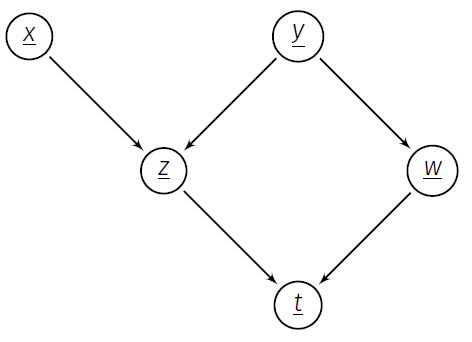
\includegraphics[width=0.4\textwidth]{figs/Graphs/simple_dag.PNG}    
    \caption{Illustration of a simple directed graph in probability.}
    \label{fig:simple_dag}
\end{figure}

% \subsubsection{Terminology}
The terms are illustrated in the figures below. 
\begin{figure}[H]
    \centering
    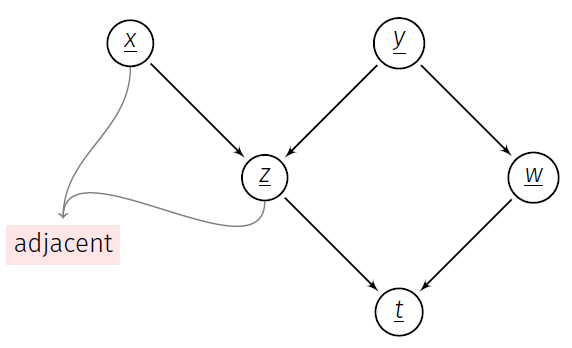
\includegraphics[width=0.4\textwidth]{figs/Graphs/dag_adjacent_vertices.PNG}    
    \caption{Directed graph terminology: adjacent vertices.}
    \label{fig:dag_adjacent_vertices}
\end{figure}
\begin{figure}[H]
    \centering
    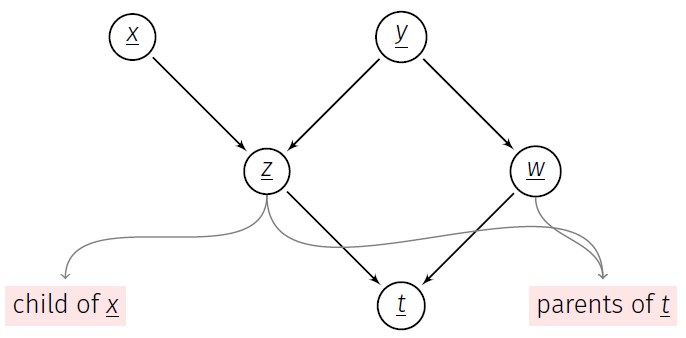
\includegraphics[width=0.4\textwidth]{figs/Graphs/dag_child_and_parent.PNG}    
    \caption{Directed graph terminology: child and parent vertices.}
    \label{fig:dag_child_and_parent}
\end{figure}
\begin{figure}[H]
    \centering
    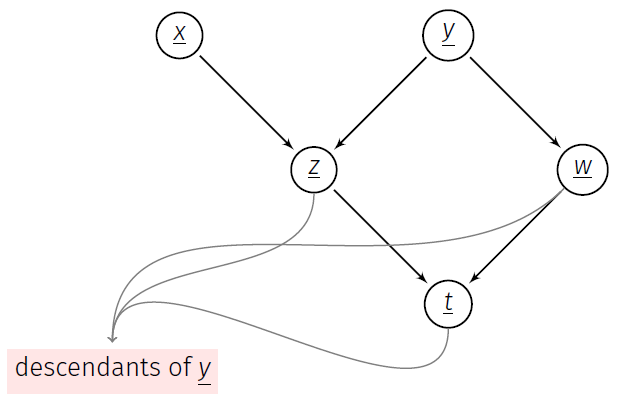
\includegraphics[width=0.4\textwidth]{figs/Graphs/dag_descendents.PNG}    
    \caption{Directed graph terminology: descendants vertices.}
    \label{fig:dag_descendents}
\end{figure}
\begin{figure}[H]
    \centering
    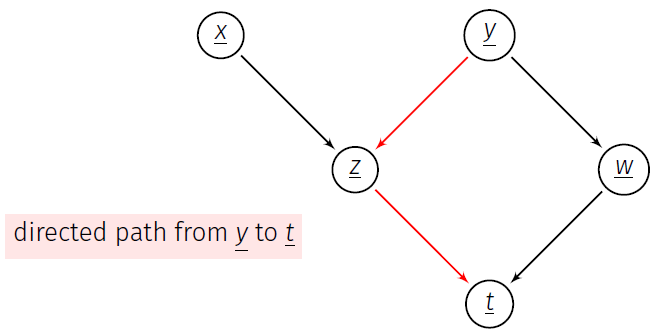
\includegraphics[width=0.4\textwidth]{figs/Graphs/dag_directed_path.PNG}    
    \caption{Directed graph terminology: directed path.}
    \label{fig:dag_directed_path}
\end{figure}
\begin{figure}[H]
    \centering
    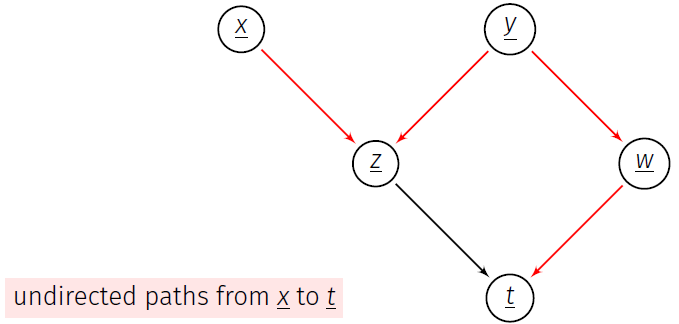
\includegraphics[width=0.4\textwidth]{figs/Graphs/dag_undirected_path.PNG}    
    \caption{Directed graph terminology: undirected path.}
    \label{fig:dag_undirected_path}
\end{figure}
\begin{figure}[H]
    \centering
    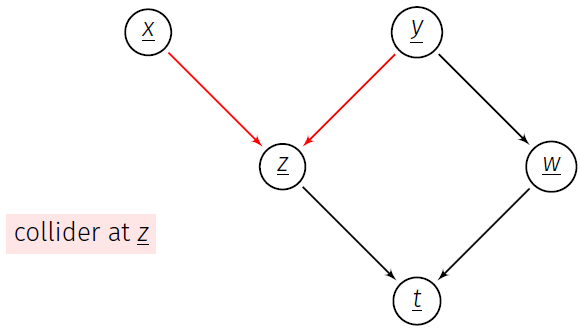
\includegraphics[width=0.4\textwidth]{figs/Graphs/dag_collider.PNG}    
    \caption{Directed graph terminology: collider.}
    \label{fig:dag_collider}
\end{figure}

\section{Graphs in Probability}
\begin{definitionBox}[Bayesian networks]
    A Bayesian network is a directed acyclic graph (DAG) (check Def.~\ref{def:directed acyclic graph}) that has random variables as vertices.
\end{definitionBox}

\begin{mytheorem}
   [Representing JPDFs using DAGs]    
   {Representing JPDFs using DAGs}
   Consider $n$ random variables $\rv{x}_{1}, \ldots, \rv{x}_{n}$ with joint pdf (JPDF) $\pdf{x_{1},\ldots,x_{n}}$. Let $G$ be a DAG with $n$ vertices representing the random variables. Then, $G$ represents the JPDF $\pdf{}$ if 
   \begin{align}
    \pdf{x_{1}, \ldots, x_{n}} &= \prod_{i=1}^{n} \pdf{x_{i}\middle|~ \text{parents of } x_{i}}.
\end{align}
\end{mytheorem}

\begin{mytheorem}
   [Markov condition in DAG]    
     The DAG $G$ represents the JPDF $\pdf{}$ if and only if the Markov condition holds, which states the following:
     \begin{align}        
         \forall \rv{x}_{i} : \quad \rv{x}_{i} \perp \bar{\mc{X}}_{i} | \text{parents of } \rv{x}_{i},
     \end{align}
     where $\bar{\mc{X}}_{i}$ are all other random variables but the parents and descendants of $\rv{x}_{i}$.
\end{mytheorem}

\begin{definitionBox}[D-donnection and d-separation]
    Consider a set of $n$ random variables $\rv{x}_{1}, \ldots, \rv{x}_{n}$ whose JPDF is represented by $G$. 
    Furthermore, let $\mc{A}$, $\mc{B}$, and $\mc{C}$ be mutually exclusive sets with $\mc{A},\mc{C}\neq\emptyset$.

    The sets $\mc{A}$ and $\mc{C}$ are called \emph{d-connected} given $\mc{B}$ if there exists an \emph{undirected} path between some random variable in $\mc{A}$ and some random variable in $\mc{C}$ such that 
    \begin{enumerate}
        \item every collider along the path is in $\mc{B}$, or has a descendent in $\mc{B}$;
        \item no non-collider along the path belongs in $\mc{B}$.
    \end{enumerate}
    If $\mc{A}$ and $\mc{C}$ are not d-connected given $\mc{B}$, then they are called \emph{d-separated given $\mc{B}$}.
\end{definitionBox}

\begin{mytheorem}
   [D-connection and d-separation] 
   Consider a set of $n$ random variables $\rv{x}_{1}, \ldots, \rv{x}_{n}$ whose JPDF is represented by $G$. Furthermore, let $\mc{A}$, $\mc{B}$, and $\mc{C}$ be mutually exclusive sets with $\mc{A},\mc{C}\neq\emptyset$. Then, 
     the sets $\mc{A}$ and $\mc{C}$ are \emph{d-separated given} $\mc{B}$ if and only if 
     \begin{align}
         \mc{A} \perp \mc{C} | \mc{B}.
     \end{align}
\end{mytheorem}

\clearpage
\part{Statistical Inference}

\chapter{Prediction}
\section{Problem statement}
Predict (guess) the value of $\mbfrv{y}$ given an \emph{observation}\footnote{Or multiple observations.} of another (related) random variable $\mbfrv{x} = \mbf{x}$. It is assumed that the JPDF $\pdf{\mbf{x},\mbf{y}}$ is known.

A prediction can be ``good'' or ``bad'' with respect to some \emph{criterion} or \emph{cost}. The objective ``\emph{best prediction}'' will refer to the \emph{minimum mean squared error} prediction.

\begin{myBlueBox}
    Note that in an estimation problem, the JPDF $\pdf{x,y}$ is not known, but observations on $\rv{x}=x$ and $\rv{y}=y$ are available.

    Furthermore, note that in the above problem statement.
\end{myBlueBox}

There are two approaches to the prediction problem:
\begin{enumerate}
    \item \textbf{Point prediction}: The objective is to identify a function $\mbf{r}(\cdot)$ so that $\mbf{r}(\mbfrv{x})$ provides a ``good'' (in some defined sense) estimate of $\rv{y}$.
    \item \textbf{Interval prediction}: Identify two function $\mbf{r}_{1}(\cdot)$ and $\mbf{r}_{2}(\cdot)$ such that 
    \begin{align}
        \prob{\mbf{r}_{1}(\mbfrv{x})<\mbfrv{y} < \mbf{r}_{2}(\mbfrv{x})} &= \gamma,
    \end{align}
    where $\gamma\in[0,1]$ is a \emph{confidence coefficient}.
\end{enumerate}
In this document, we will be concerned with point prediction. 

\begin{myBlackBox}
    Note that the function $r(\cdot)$ is determined before any observation is made! The goal is to \emph{guess} $r(\cdot)$ to be good over \emph{all} possible observations of $\rv{x}$ and the associated true value of $\rv{y}$.
\end{myBlackBox}

\section*{Terminology}
\begin{itemize}
    \item \emph{Estimate of $\mbfrv{y}$}: the deterministic value of $\mbf{r}(\mbf{x})$ obtained by applying $\mbf{r}(\cdot)$ on the observed value of $\mbfrv{x}$, $\mbf{x}$.
    \item \emph{Predictor} or \emph{estimator} of $\mbfrv{y}$: the random random variable $\mbf{r}(\mbfrv{x})$ obtained by applying $\mbf{r}(\cdot)$ on the random variable $\mbfrv{x}$.
    \item Notation to be used: 
    \begin{align}
        \mbf{r}(\mbfrv{x}) \to \hat{\mbfrv{y}}.
    \end{align}
\end{itemize}

\section{MMSE Prediction}
\begin{mydefinition}[Mean-Squared Predictor]
    The \emph{mean-squared predictor} of $\mbfrv{y}$ from $\mbfrv{x}$, is the function $r(\cdot)$ that minimizes the mean-square error (MSE):
    \begin{align}
        \expect{\norm{\mbfrv{y} - \mbf{r}(\mbfrv{x})}^{2}}
        \expect{\left( \mbfrv{y} - \mbf{r}(\mbfrv{x}) \right)^{\trans} \left( \mbfrv{y} - \mbf{r}(\mbfrv{x}) \right)}
    \end{align}
\end{mydefinition}

\begin{mytheorem}
   [Constant-value predictor]    
     The mean square predictor of $\mbf{y}$ \emph{by a constant} $\mbf{r}(\mbfrv{x}) = \mbf{c}$ is given by
     \begin{align}
         \mbf{c} &= \expect{\mbfrv{y}}.
     \end{align}
\end{mytheorem}
\begin{proof}
    Let $\mbf{e}(\mbf{c}) := \expect{\norm{\mbfrv{y} - \mbf{r}(\mbfrv{x})}^{2}}$. Then, the derivative of $\mbf{e}$ w.r.t. $\mbf{c}$ (the design variable) is 
    \begin{align}
        \td{\mbf{e}(\mbf{c})}{\mbf{c}} &= \td{}{\mbf{c}}  \expect{\left( \mbfrv{y} - \mbf{c} \right)^{2})}\\
        &= 
        -2
        \mbf{c}^{\trans}
        \expect{
          \left( \mbfrv{y} - \mbf{c} \right))  
        }.
    \end{align}
    Setting $\td{\mbf{e}(\mbf{c})}{\mbf{c}} = \mbf{0}$, gives the relation 
    \begin{align}
        \mbf{c}^{\trans}\expect{\mbfrv{y}} &= \mbf{c}^{\trans}\mbf{c}.
    \end{align}
    A nontrivial solution is
    \begin{align}
        \mbf{c} &= \expect{\mbfrv{y}}.
    \end{align}
\end{proof}

\begin{mytheorem}
   [Mean-squared predictor]    
   The mean-squared predictor of $\mbfrv{y}$ given $\mbfrv{x}$ is     
   \begin{align}
       \mbf{r}(\mbfrv{x}) &= \expect[\mbf{y}|\mbf{x}]{\mbfrv{y}\middle|~\mbfrv{x}}.
   \end{align}
\end{mytheorem}
\begin{proof}
    MSE of $\mbf{r}(\mbf{x})$.
\end{proof}

\begin{myremark}
    Some remarks on MMSE prediction.
    \begin{enumerate}
        \item If $\mbfrv{y}=\mbf{h}(\mbfrv{x})$ then 
        $\expect[\mbf{y}]{\mbfrv{y}\middle|~\mbfrv{x}} = \mbf{h}\left( \mbfrv{x} \right))$, and the resulting MSE is $\mbf{0}$.
        
        \item If $\mbfrv{y}$ and $\mbfrv{x}$ are independent then $\expect[\mbf{y}]{\mbfrv{y}\middle|~\mbfrv{x}}=\expect{\mbfrv{y}} = \text{constant}$.
    \end{enumerate}
\end{myremark}

\begin{mytheorem}
   If $\mbfrv{y}$, $\mbfrv{x}_{1}, \ldots, \mbfrv{x}_{N}$ are jointly normal with zero mean, the linear and non-linear predictors of $\mbfrv{y}$ from $\mbfrv{x}_{1},\ldots, \mbfrv{x}_{N}$.     
\end{mytheorem}

\chapter{Parameter Estimation}
\section{Motivation}
Let $\rv{x}$ be a random variable whose CDF, $\cdf{x}$, \emph{is unknown}. The goal is estimate $\cdf{x}$ from $n$ observations of $\rv{x}$, $x_{1}, \ldots, x_{n}$.

\begin{definitionBox}[Empirical CDF]
    The empirical CDF of $\rv{x}$ from the observations $x_{1}, \ldots, x_{n}$ is
    \begin{align}
        \hat{\cdf{}}(x) &= \f{1}{n} \times \left( \# \text{ of observations } x_{i} \leq x \right).
    \end{align}
\end{definitionBox}
The empirical CDF $\hat{\cdf{}}(x)$ is the CDF of a discrete random variable with PMF
\begin{align}
    \hat{\pmf{}}_{n}(x) &= 
    \begin{cases}
        \f{1}{n}, & x = x_{i}, \quad i = 1,\ldots, n,\\
        0 & \text{Otherwise}.
    \end{cases}
\end{align}
The PDF is then given by
\begin{align}
    \label{eq:empirical pdf constant weight}
    \hat{\pdf{}}_{n}(x) &= \sum_{i=1}^{n}\f{1}{n}\delta(x-x_{i}).
\end{align}

The empirical PDF $\hat{\pdf{}}(x)$ in \eqref{eq:empirical pdf constant weight} assigns constant weights to every observation. The empirical PDF can be generalized by giving different weights to different observations. Specifically,
\begin{align}
    \hat{\pdf{}}_{n}(x) &= \sum_{i=1}^{n}\f{1}{n}k(x-x_{i}),
\end{align}
where $k(\cdot)$ is the kernel function such that it is
\begin{enumerate}
    \item symmetric around 0, and
    \item $\int_{-\infty}^{\infty}k(x)\dee x = 1$.
\end{enumerate}
A common choice is the Gaussian kernel. That is, a PDF of $\mc{N}(0,1)$.


%%%%%%%%%%%%%%%%%%%%%%%%%%%%%%%%%%%%%%%%%%%%%%%%%%%%%%%%%%%%%%%%%%%%%%%%%%%%%%%%%%%%
% Parameter estimation
%%%%%%%%%%%%%%%%%%%%%%%%%%%%%%%%%%%%%%%%%%%%%%%%%%%%%%%%%%%%%%%%%%%%%%%%%%%%%%%%%%%%
\section{Problem statement}
Let $\mbfrv{x}$ be a random variable. Furthermore, let $\pdf{\mbf{x}; \mbs{\theta}}$ be the PDF of $\mbfrv{x}$ of \emph{known form} (\eg, Gaussian distribution) but depending on \emph{unknown} parameters $\mbs{\theta}$ (\eg, mean and covariance of a Gaussian distribution).
\begin{example}
    A Gaussian random variable has a PDF parameterized w.r.t. to the mean ${\mu}$ and the variance $\sigma^{2}$. Thus, the parameters could be $\mbs{\theta} = \bbm \mu, \sigma^{2} \ebm$.
\end{example}

The goal is to estimate $\mbs{\theta}$ from $n$ observations of $\mbfrv{x}$: $\mbf{x}_{1}, \ldots, \mbf{x}_{n}$. 

Define the data vector 
\begin{align}
    \mbf{X} &= \bbm \mbf{x}_{1}\\\vdots\\\mbf{x}_{n} \ebm.
\end{align}
The data vector $\mbf{X}$ is a realization of the random vector 
\begin{align}
    \mbfrv{X} &= \bbm \mbfrv{x}_{1} \\ \vdots \\ \mbfrv{x}_{n} \ebm,
\end{align}
where $\mbfrv{x}_{i}$, $i=1,\ldots, n$ are i.i.d.

\subsection*{Approaches}
There are two approaches to parameter estimation.
\begin{enumerate}
    \item \emph{Point estimation}: identify a function $g(\cdot)$ of the sample such that $g(\mbfrv{x}_{1},\ldots, \mbfrv{x}_{n})$ is a good (in some sense) approximation of $\mbs{\theta}$.
    \item \emph{Interval estimation}: identify two functions $g_{1}(\cdot)$ and $g_{2}(\cdot)$ of the sample, such that
    \begin{align}
        \prob{g_{1}(\mbfrv{x}_{1},\ldots,\mbfrv{x}_{n})<\mbs{\theta}<g_{2}(\mbfrv{x}_{1},\ldots,\mbfrv{x}_{n})} = \gamma,
    \end{align}
    where $\gamma$ is the confidence interval.
\end{enumerate}

\section{Definitions and terminology}
\begin{definitionBox}[Estimator]
    The estimator of $\mbs{\theta}$ is given in the form
    \begin{align}
        \hat{\mbsrv{\theta}} &= g(\mbfrv{x}_{1}, \ldots, \mbfrv{x}_{n}).
    \end{align}

    The estimator models the behaviour of the estimation method over all possible samples.
\end{definitionBox}
\begin{definitionBox}[Estimate of $\mbs{\theta}$]
    The \emph{deterministic} quantity $g(\mbf{x}_{1},\ldots,\mbf{x}_{n})$. That is, the the output of $\hat{\mbsrv{\theta}}$ for the realizations $\mbf{x}_{1}, \ldots, \mbf{x}_{n}$.
\end{definitionBox}
\begin{definitionBox}[Statistic]
    Any function of $\mbfrv{x}_{1}, \ldots, \mbfrv{x}_{n}$.
\end{definitionBox}
\begin{definitionBox}[Bias]
    The estimator $g(\mbfrv{x}_{1}, \ldots, \mbfrv{x}_{n})$ is called
    \begin{itemize}
        \item \emph{unbiased} if 
        \begin{align}
            \expect{g(\mbfrv{x}_{1},\ldots, \mbfrv{x}_{n})} &= \mbs{\theta}.
        \end{align}
        \item Otherwise, it's called \emph{biased} with bias
        \begin{align}
            \expect{g(\mbfrv{x}_{1},\ldots, \mbfrv{x}_{n})} - \mbs{\theta}.
        \end{align}
    \end{itemize}
\end{definitionBox}

\begin{definitionBox}[Asymptic unbias]
    A biased estimator for which
    \begin{align}
        \expect{g(\mbfrv{x}_{1},\ldots,\mbfrv{x}_{n})} \overset{N\to\infty}{\to} \mbs{\theta}
    \end{align}
    is called \emph{asymptotically unbiased}.
\end{definitionBox}

\begin{definitionBox}[Mean-squared best estimator]
   For a fixed $n$, the estimator that minimizes the mean-squared (MS) error 
   \begin{align}
       \mbf{e}_{n} &= \expect{\abs{g(\mbfrv{x}_{1},\ldots\mbfrv{x}_{n})^{\trans}g(\mbfrv{x}_{1},\ldots\mbfrv{x}_{n})}}
   \end{align}
   is called the \emph{best} estimator (in the mean-squared sense).
\end{definitionBox}

\begin{definitionBox}[Consistency]
    The estimator $g(\mbfrv{x}_{1},\ldots\mbfrv{x}_{n})$ is called \emph{consistent} if 
    \begin{align}
        \lim_{n\to\infty} \prob{\abs{g(\mbfrv{x}_{1},\ldots\mbfrv{x}_{n})}>\mbs{\epsilon}} &= 0, \forall \mbs{\epsilon}>\mbf{0},
    \end{align}
    or
    \begin{align}
        \lim_{n\to\infty} \prob{\abs{g(\mbfrv{x}_{1},\ldots\mbfrv{x}_{n})}<\mbs{\epsilon}} &= 1, \forall \mbs{\epsilon}>\mbf{0}.
    \end{align}
\end{definitionBox}

\begin{mytheorem}
    [Sufficient condition for consistency]    
    Let $g(\mbfrv{x}_{1},\ldots\mbfrv{x}_{n})$ be an estimator of $\mbs{\theta}$. Then, if
    \begin{align}
        \lim_{n\to\infty} \expect{\abs{g(\mbfrv{x}_{1},\ldots\mbfrv{x}_{n})^{\trans}g(\mbfrv{x}_{1},\ldots\mbfrv{x}_{n})}} &= \mbf{0},
    \end{align}
    then $g(\mbfrv{x}_{1},\ldots\mbfrv{x}_{n})$ is a \emph{consistent estimator} of $\mbs{\theta}$.

    The converse is not true in general. That is, this is a sufficient but not necessary condition.
\end{mytheorem}


\begin{mytheorem}
   [Sample mean estimator]    
     Let $\mbfrv{x}_{1},\ldots, \mbfrv{x}_{n}$ be a random sample of size $n$ and let $\mbfrv{x}_{1},\ldots, \mbfrv{x}_{n}$ be \emph{uncorrelated}. The \emph{sample mean estimator}
     \begin{align}
         \hat{\mbsrv{\mu}}_{n} &= \f{1}{n}\sum_{i=1}^{n}\mbfrv{x}_{i}
     \end{align}
     is
     \begin{itemize}
         \item an \emph{unbiased estimator} of $\mbs{\mu}$;
         \item a \emph{consistent estimator} of $\mbs{\mu}$.
     \end{itemize}
\end{mytheorem}

\begin{mytheorem}
   [Variance estimaton]    
   Consider the sample average estimators of the mean and variance of Gaussian random variable $\rv{x}$ from a random sample $\rv{x}_{1},\ldots, \rv{x}_{n}$ of size $n$:
   \begin{align}
       \hat{\rv{\mu}}_{n} &= \f{1}{n}\sum_{i=1}^{n}\rv{x}_{i},\\
       \hat{\rv{\sigma}}_{n}^{2} &= \f{1}{n} \sum_{i=1}^{n}\left( \rv{x}_{i}-\hat{\rv{\mu}}_{n} \right)^{2}.
   \end{align}
   The random variables $\hat{\rv{\mu}}_{n}$ and $\hat{\rv{sigma}}_{n}^{2}$ are independent.
\end{mytheorem}

\section{Method of moments}
Recall that moments are defined in Def.~\ref{def:moments single rv} and Def.~\ref{def:moments multiple rv}. 
The $m$-th moment estimator is given by
\begin{align}
    \hat{m}_{m}(\mbf{X}) &= 
    \f{1}{n}\sum_{i}^{n}x_{i}^{m}.
\end{align}
Let $\mbs{\theta}\in\rnums^{k}$ be of size $k$ and let 
\begin{align}
    \mbf{X} &= \bbm x_{1} \\\vdots\\x_{n} \ebm 
\end{align}
be the samples of the random variable $\rv{x}$. Then, 
the idea of method of moments is to estimate the first $k$ moments, thus getting $k$ equations, and then solving the $k$ equations for $\mbs{\theta}$.

\begin{example}
    Estimate the mean $\mu$ and variance $\sigma^{2}$ of a random variable $\rv{x}$ from a random sample $\mbfrv{X} = \bbm \rv{x}_{1}&\ldots&\rv{x}_{n} \ebm^{\trans}$.

    The moments are given by
    \begin{alignat}{2}
        m_{1}(\mu, \sigma^{2}) &= \expect{\rv{x}} &&= \mu, \\
        m_{2}(\mu, \sigma^{2}) &= \expect{\rv{x}^{2}} &&= \mu^{2} + \sigma^{2}.
    \end{alignat}
    The sample average estimates of the moments are given by
    \begin{align}
        \hat{m}_{1}(\mbf{X}) &= \f{1}{n}\sum_{i=1}^{n}x_{i},\\
        \hat{x}_{2}(\mbf{X}) &= \f{1}{n}\sum_{i=1}^{n}x_{i}^{2}.
    \end{align}
    Thus, the parameter estimates can be computed by solving the system of equations
    \begin{align}
        \mu &= \hat{m}_{1}(\mbf{X})\\
        \mu^{2} + \sigma^{2} &= \hat{m}_{2}(\mbf{X}).
    \end{align}
    The solution is given by
    \begin{align}
        \hat{\mu} &= \hat{m}_{1}(\mbf{X}) \\
            &= \f{1}{n}\sum_{i=1}^{n}x_{i},\\
        \hat{\sigma}^{2} &= \hat{m}_{2}(\mbf{X}) - \hat{m}_{1}^{2}(\mbf{X})\\
        &= \f{1}{n}\sum_{i=1}^{n}x_{i}^{2}  - \left(\f{1}{n}\sum_{i=1}^{n}x_{i}\right)^{2}.
    \end{align}
\end{example}


%%%%%%%%%%%%%%%%%%%%%%%%%%%%%%%%%%%%%%%%%%%%%%%%%%%%%%%%%%%%%%%%%%%%%%%%%%%%%%%%%%%%
% Maximum likelihood
%%%%%%%%%%%%%%%%%%%%%%%%%%%%%%%%%%%%%%%%%%%%%%%%%%%%%%%%%%%%%%%%%%%%%%%%%%%%%%%%%%%%
\section{Maximum likelihood (ML) estimator}
\begin{definitionBox}[Likelihood]
    Given the observations $\mbfrv{x}_{1} = \mbf{x}_{1}', \ldots, \mbfrv{x}_{n}=\mbf{x}_{n}'$, the \emph{likelihood} of $\mbs{\theta}$ is the joint PDF of $\mbfrv{x}_{1},\ldots,\mbfrv{x}_{n}$ evaluated at the observed points
    \begin{align}
        L(\mbs{\theta}; \mbf{x}_{1}', \ldots, \mbf{x}_{N}') &=
        \pdf{\mbf{x}_{1}',\ldots, \mbf{x}_{n}';\mbs{\theta}}\\
         &= \pdf{}_{\mbf{x}}(\mbf{x}_{1}';\mbs{\theta})\cdots\pdf{}_{\mbf{x}}(\mbf{x}_{n}';\mbs{\theta}).
    \end{align}
\end{definitionBox}
\begin{myremark}
    \begin{itemize}
        \item The likelihood $\pdf{\mbf{x}_{1}',\ldots, \mbf{x}_{n}';\mbs{\theta}}$ is treated as a function of $\mbs{\theta}$.
        \item It is not a PDF. That is,
        \begin{align}
            \int_{-\infty}^{\infty}\pdf{\mbf{x}_{1}',\ldots, \mbf{x}_{n}';\mbs{\theta}}\dee\mbs{\theta}\neq 1.
        \end{align}
    \end{itemize}
\end{myremark}

\begin{definitionBox}[Maximum-likelihood estimator]
    The maximum-likelihood (ML) estimate of $\mbs{\theta}$, $\hat{\mbs{\theta}}_{\mathrm{ML}}$, is the value of $\mbs{\theta}$ that maximizes $\pdf{\mbf{x}_{1}',\ldots, \mbf{x}_{n}';\mbs{\theta}}$. That is,
    \begin{align}
        \hat{\mbs{\theta}}_{\mathrm{ML}} 
        &= \argmax_{\mbs{\theta}\in\rnums^{k}} L(\mbs{\theta}; \mbf{x}_{1}', \ldots, \mbf{x}_{N}')\\
        &= \argmax_{\mbs{\theta}\in\rnums^{k}} \pdf{\mbf{x}_{1}',\ldots, \mbf{x}_{n}';\mbs{\theta}}.
    \end{align}
\end{definitionBox}

\begin{myremark}
    Some remarks regarding the ML estimator.
    \begin{itemize}
        \item Log-likelihood function 
        \begin{align}
            \ell(\mbf{x}_{1}',\ldots,\mbf{x}_{n}';\mbs{\theta}) 
            &= \log L(\mbs{\theta}; \mbf{x}_{1}', \ldots, \mbf{x}_{N}')\\
            &= \log \pdf{\mbf{x}_{1}',\ldots, \mbf{x}_{n}';\mbs{\theta}}.
        \end{align}
        \item The maximizer of the log-likelihood function is the same maximizer of the likelihood function. That is,
        \begin{align}
            \argmax_{\mbs{\theta}\in\rnums^{k}} L(\mbs{\theta}; \mbf{x}_{1}', \ldots, \mbf{x}_{N}')
            &= \argmax_{\mbs{\theta}\in\rnums^{k}} \ell(\mbs{\theta}; \mbf{x}_{1}', \ldots, \mbf{x}_{N}').
        \end{align}
        \item The ML estimate is 
        \begin{align}
            \hat{\mbs{\theta}}_{\mathrm{ML}} 
            &= \argmax_{\mbs{\theta}\in\rnums^{k}} \pdf{\mbf{x}_{1}',\ldots, \mbf{x}_{n}';\mbs{\theta}}\\
            &= \argmax_{\mbs{\theta}\in\rnums^{k}} \log \pdf{\mbf{x}_{1}',\ldots, \mbf{x}_{n}';\mbs{\theta}}\\
            &= \argmax_{\mbs{\theta}\in\rnums^{k}} L(\mbf{x}_{1}',\ldots,\mbf{x}_{n}';\mbs{\theta}).
        \end{align}
    \end{itemize}
\end{myremark}

\begin{myremark}
    Some remarks on ML estimation.
    \begin{enumerate}
        \item Let $\hat{\mbsrv{\theta}}_{\mathrm{ML}}$ be the ML estimator of $\mbs{\theta}$ and let $g(\mbs{\theta})$ be a function of $\mbs{\theta}$. Then, the ML estimator of $g(\mbs{\theta})$ is $g(\hat{\mbsrv{\theta}}_{\mathrm{ML}})$.
        
        \item Limitations of the ML estimation:
        \begin{enumerate}
            \item The ML estimate may not exist.
            \item The ML estimate may not be unique. 
        \end{enumerate}        
        
        \item Maximum likelihood estimate can be finding by minimizing the negative likelihood or negative log-likelihood.
    \end{enumerate}
\end{myremark}
    
\begin{example}
    Let $\rv{x}\sim U[0,\theta]$ be a uniformly distributed random variable in the form
    \begin{align}
        \pdf{x; \theta} &= 
        \begin{cases}
            \f{1}{\theta}, &x\in[0,\theta],\\
            0,&\text{otherwise},
        \end{cases}
    \end{align}
    where $\theta$ is some unknown parameter. Find the ML estimator of $\theta$ from a random sample of size $N$.

    \begin{enumerate}
        \item First, get the joint PDF of all the random samples
        \begin{align}
            \pdf{x_{1}, \ldots, x_{N}; \theta} &= \pdf{x_{1};\theta}\cdots\pdf{x_{N}; \theta}\\
            &= 
            \begin{cases}
                \f{1}{\theta^{N}}, &x_{i}\in[0, \theta], i=1,\ldots,N,\\
                0, &\text{otherwise},
            \end{cases}
        \end{align}
        where the fact that the random samples $\rv{x}_{i}$ for $i=1,\ldots,N$ are i.i.d. 

        \item The likelihood of $\theta$ is then given as a function of the samples of $\rv{x}_{i}=x_{i}'$. Specifically, the likelihood is
        \begin{align}
            L(\theta; x_{1}', \ldots, x_{N}') &=
            \pdf{\rv{x}_{1} = x_{1}', \ldots, \rv{x}_{N} = x_{N}'; \theta}\\
            &=
            \begin{cases}
                \f{1}{\theta^{N}}, &x_{i}'\in[0,\theta], i=1,\ldots, N, \\
                0, &\text{otherwise}
            \end{cases}\\
            &=
            \begin{cases}
                \label{eq:example ML uniform distribution}
                \f{1}{\theta^{N}}, &\max_{i}(x_{i})\leq\theta, \\
                0, &\text{otherwise}.
            \end{cases}
        \end{align}
        Note that it was not necessary to specify the lower bound $\min_{i}(x_{i})\geq 0$ since the samples are drawn from a uniform distribution $U[0, \theta]$ which is bounded from below by $0$. Thus, $\prob{\rv{x}<0} = 0$. Therefore, it is impossible to have a sample $x_{i}'<0$.

        \item Maximize the likelihood function. Maximizing \eqref{eq:example ML uniform distribution} is a \emph{constrained} optimization problem that entails maximizing $\f{1}{\theta^{N}}$. 
        
        Maximizing $\f{1}{\theta^{N}}$ is the same as minimizing $\theta$. However, since $\theta$ is bounded from below by the constraint in \eqref{eq:example ML uniform distribution}, then the minimum value of $\theta$ is $\max_{i}(x_{i})$. Thus,
        \begin{align}
            \hat{\theta}_{\mathrm{ML}} &= \max_{i}(x_{i}).
        \end{align}
    \end{enumerate}
    \triqed
\end{example}
\section{Bayesian parameter estimation}
% \subsection*{Introduction and terminology}
In the previous sections, the approaches used were the \emph{classical} or \emph{frequentist} approaches. The classical approach
\begin{enumerate}
    \item treats the unknown parameter as deterministic parameter, and
    \item assumes no prior information on the unknown parameter was available.
\end{enumerate}

For Bayesian approach on the other hand
\begin{enumerate}
    \item assumes that unknown parameter is random with known pdf $\pdf{\mbs{\theta}}$, called the \emph{prior};
    \item the JPDF of random sample given $\mbsrv{\theta} = \theta$ (likelihood) is given by
    \begin{align}
        \pdf{\mbf{x}_{1},\ldots,\mbf{x}_{n}\middle|~ \mbs{\theta}};
    \end{align}
    \item The estimation problem becomes a prediction problem; predict $\mbsrv{\theta}$ from a correlated (with $\mbsrv{\theta}$) sample $\mbfrv{X}$.
\end{enumerate}

The mean-squared (or Bayes) estimate $\hat{\mbs{\theta}}$ of $\mbsrv{\theta}$ given $\mbfrv{X}=\mbf{X}$ is
\begin{align}
    \label{eq:bayesian estimator E(theta|X)}
    \hat{\mbs{\theta}} &= \expect{\mbsrv{\theta}\middle|~\mbf{X}}\\
    &= \int_{-\infty}^{\infty}\mbs{\theta}\pdf{\mbs{\theta}\middle|~\mbf{X}}\dee\mbs{\theta},
\end{align}
where
\begin{align}
    \pdf{\mbs{\theta}\middle|~\mbf{X}} &= 
        \f{
            \pdf{\mbf{X}\middle|~\mbs{\theta}}\pdf{\mbs{\theta}}
        }{\pdf{\mbf{X}}}\\
    &=
        \f{
            \pdf{\mbf{X}\middle|~\mbs{\theta}}\pdf{\mbs{\theta}}
        }{
            \int_{-\infty}^{\infty}\pdf{\mbf{X}\middle|~\mbs{\theta}}\pdf{\mbs{\theta}}\dee\mbs{\theta}
        }.
\end{align}

\begin{myBlueBox}
    \textbf{Terminology}
    \begin{itemize}
        \item The mean-squared estimator is also referred to as the Bayes estimator.
        \item $\pdf{\mbs{\theta}}$: \emph{prior} pdf of $\mbsrv{\theta}$ (before observing the sample).
        \item $\pdf{\mbs{\theta}\middle|~\mbf{X}}$: \emph{posterior} pdf of $\mbs{\theta}$ (after observing the sample).
        \item In \cite{barfoot_state_2017}, the term $\pdf{\mbf{X}\middle|~\mbs{\theta}}$ is sometimes referred to as the likelihood of $\mbf{X}$ given $\mbs{\theta}$. This is not to be confused with the likelihood from the ML estimator. In estimation, the term $\pdf{\mbf{X}\middle|~\mbs{\theta}}$ can also be referred to as an \emph{observation model}. 
    \end{itemize}
\end{myBlueBox}

\begin{myremark}
    Some remarks about Bayesian estimation.    
    \begin{itemize}
        \item $\expect{\mbsrv{\theta}\middle|~\mbf{X}}$ from \eqref{eq:bayesian estimator E(theta|X)} is difficult to solve for two reasons. First, the denominator of the posterior pdf involves evaluating an integral over the entire sample space of $\mbs{\theta}$. Second, evaluating the expectation $\expect{\cdot}$ requires \emph{another} integral to be evaluated over the entire sample space.
        
        \item Maximum a-posteriori (MAP) estimate maximizes the \emph{posterior} pdf $\pdf{\mbs{\theta}\middle|~\mbf{X}}$ with respect to $\mbs{\theta}$. Since the denominator of the prior is constant, then it can be omitted. That is,
        \begin{align}
            \hat{\mbs{\theta}}_{\mathrm{MAP}} 
            &= \argmax_{\mbs{\theta}} \pdf{\mbs{\theta}\middle|~\mbf{X}}\\
            &= \argmax_{\mbs{\theta}} \f{\pdf{\mbf{X}\middle|~\mbs{\theta}}\pdf{\mbs{\theta}}}{\pdf{\mbf{X}}}\\
            &= \argmax_{\mbs{\theta}} \pdf{\mbf{X}\middle|~\mbs{\theta}}\pdf{\mbs{\theta}}.
        \end{align}
    \end{itemize}
\end{myremark}

\section{Maximum a-posteriori (MAP) estimator}
This estimator is an \emph{approximation} to the Bayes estimator discussed in the previous section. It is easier (less computationally intensive) to compute.
\begin{definitionBox}[Maximum a-posteriori estimator]
    Maximum a-posteriori (MAP) estimate maximizes the \emph{posterior} pdf $\pdf{\mbs{\theta}\middle|~\mbf{X}}$ with respect to $\mbs{\theta}$. Since the denominator of the prior is constant, then it can be omitted. That is,
        \begin{align}
            \hat{\mbs{\theta}}_{\mathrm{MAP}} 
            &= \argmax_{\mbs{\theta}} \pdf{\mbs{\theta}\middle|~\mbf{X}}\\
            &= \argmax_{\mbs{\theta}} \f{\pdf{\mbf{X}\middle|~\mbs{\theta}}\pdf{\mbs{\theta}}}{\pdf{\mbf{X}}}\\
            &= \argmax_{\mbs{\theta}} \pdf{\mbf{X}\middle|~\mbs{\theta}}\pdf{\mbs{\theta}}.
        \end{align}
\end{definitionBox}

\subsection{MAP estimator of a Markov normally distributed random variable}

In this section, the MAP estimator for normally distributed variables that follow a Markov chain will be derived. For each problem, a process model is provided in the form 
\begin{align}
    \label{eq:MAP state estimation process model}
    \mbfrv{x}_{k+1} &= \mbfrv{f}(\mbf{x}_{k}, \mbfrv{u}_{k}, \mbfuline{w}_{k}),
\end{align}
where $\mbfuline{w}_{k}\sim\mc{N}(\mbf{0},\mbf{Q}_{k})$ is the process noise and the covariance matrix $\mbf{Q}_{K}$ is known. A prior is distributed according to $\mbfhat{x}_{0}\sim\mc{N}\left( \mbfhat{x}_{1}, \mbfcheck{P}_{0} \right)$.

Furthermore, a measurement model is given in the form
\begin{align}
    \label{eq:MAP state estimation measurement model}
    \mbfrv{y}_{k} &= \mbf{g}(\mbfrv{x}_{k}, \mbfuline{v}_{k}),
\end{align}
where $\mbfuline{v}_{k}\sim\mc{N}(\mbf{0},\mbf{R}_{k})$ is the Gaussian measurement noise, where the covariance matrix $\mbf{R}_{k}$ is known. 

The goal is to estimate states' $\mbfrv{x}_{1:K}$ parameters using the realizations of the prior $\mbf{x}_{0}$, the realizations of the interoceptive measurements $\mbf{u}_{k}$ and realizations of the exteroceptive measurements $\mbf{y}_{k}$. If the RVs are Gaussian, then they can be parametrized by a mean and a covariance (\ie, $\mbfrv{x}_{k}\sim\mc{N}(\mbs{\mu}_{k}, \mbs{\Sigma}_{k})$). 

\begin{myremark}
    The interoceptive measurement $\mbfrv{u}_{k}$ is a random variable that can be assumed to be distributed according to
    \begin{align}
        \mbfrv{u}_{k}\sim\mc{N}\left( \mbf{u}_{k}, \mbf{Q}_{k}^{\mbf{u}} \right).
    \end{align}
    The measurement is assumed to be random due to measurement noise. However, the measurement noise can be embedded into the process noise $\mbf{Q}$. Therefore, it is possible to assume that the interoceptive measurements are not random, but the interoceptive measurement process noise is indeed random and will be embedded with the process noise $\mbfrv{w}_{k}$.
\end{myremark}
\begin{myremark}
    The states will be assumed to be normally distributed. That is, $\mbfrv{x}_{k}\sim\mc{N}\left( \mbf{x}_{k}, \mbf{P}_{k} \right)$. Therefore, the parameters to be estimated should
    \begin{align}
        \tilde{\mbs{\theta}} &= \left\{ \mbf{x}_{0}, \ldots, \mbf{x}_{N}, \mbf{P}_{0}, \ldots, \mbf{P}_{N}\right\}.
    \end{align}
    However, to make things easier, the covariances $\mbf{P}_{0:N}$ will not be estimated (they will be computed after the MAP estimate is computed). Thus, the parameters that'll be estimated is given by
    \begin{align}
        \mbs{\theta} &= \left\{ \mbf{x}_{0}, \ldots, \mbf{x}_{N}\right\}.
    \end{align}
    The realizations are then
    \begin{align}
        \mbf{X} &= \left\{ \mbfcheck{x}_{0}, \mbf{u}_{0:N-1}, \mbf{y}_{1:N}\right\}.
    \end{align}
\end{myremark}
For the MAP estimator, the PDF of interest is
\begin{align}
    \pdf{\mbs{\theta}\middle|~ \mbf{X}} 
    \label{eq:MAP state estimation f(theta|X)}
    &= \pdf{\mbf{x}_{0}, \ldots, \mbf{x}_{N} \middle|~ \mbfcheck{x}_{0}, \mbf{u}_{0:N-1}, \mbf{y}_{1:N}} \\
    &= \f{\pdf{\mbf{y}_{1:N}\middle|~ \mbf{x}_{0:N}, \mbfcheck{x}_{0}, \mbf{u}_{0:N-1}}\pdf{\mbf{x}_{0:N}\middle|~\mbfcheck{x}_{0}, \mbf{u}_{0:N-1}}}{\pdf{\mbf{y}_{1:N}\middle|~ \mbfcheck{x}_{0}, \mbf{u}_{0:N-1}}}\\
    &= \eta \pdf{\mbf{y}_{1}\middle|~ \mbf{x}_{1}}\cdots\pdf{\mbf{y}_{N}\middle|~\mbf{x}_{N}}
        \pdf{\mbf{x}_{N}\middle|~\mbf{x}_{N-1}, \mbf{u}_{N-1}}\cdots\pdf{\mbf{x}_{1}\middle|~\mbf{x}_{0}, \mbf{u}_{0}}\pdf{\mbf{x}_{0} \middle|~ \mbfcheck{x}_{0}}\\
    \label{eq:MAP state estimation f(y|x)f(x|xm1)}
    &= \eta \prod_{k=1}^{N}\pdf{\mbf{y}_{k}\middle|~\mbf{x}_{k}}\prod_{k=1}^{N}\pdf{\mbf{x}_{k}\middle|~\mbf{x}_{k-1}, \mbf{u}_{k-1}} \pdf{\mbf{x}_{0}, \middle|~ \mbfcheck{x}_{0}},
\end{align}
where $\eta$ is a normalizing parameter that is independent of the design variables ($\mbf{x}_{0:N}$) and the following assumptions were used
\begin{enumerate}
    \item The measurements $\mbf{y}_{k}$ depends only on $\mbf{x}_{k}$ (and measurement noise $\mbfrv{n}_{k}$ )as shown in the measurement model \eqref{eq:MAP state estimation measurement model}. Thus, the random variable $\mbfrv{y}_{k}$ is independent of all other random variables. 
    
    \item The state $\mbfrv{x}_{k}$ depends only on $\mbfrv{x}_{k-1}$ and $\mbf{u}_{k-1}$ (and process noise $\mbfrv{w}_{k-1}$) as shown in \eqref{eq:MAP state estimation process model}. Therefore, the random variables $\mbf{x}_{0:N}$ follow the \textbf{Markov sequence}: the future states $\mbfrv{x}_{k+1:N}$ are independent of the past states $\mbfrv{x}_{0:k-1}$ given the present state $\mbfrv{x}_{k}$. The Markov sequence is dictated by the process model \eqref{eq:MAP state estimation process model}.
        
\end{enumerate}

If $\mbfrv{x}_{0:N}$ are assumed to be [marginally] Gaussian, then it is easier to minimize the negative-log of \eqref{eq:MAP state estimation f(theta|X)} than maximize \eqref{eq:MAP state estimation f(theta|X)} directly. 

Taking the negative-log of \eqref{eq:MAP state estimation f(y|x)f(x|xm1)} gives
\begin{align}    
    -\log \pdf{\mbf{x}_{0:N}\middle|~ \mbfcheck{x}_{0}, \mbf{u}_{0:N-1}, \mbf{y}_{1:N}}
    \label{eq:negative log likelihood}
    &=
    \f{1}{2}\norm{\mbf{x}_{0} - \mbfcheck{x}_{0}}^{2}_{\mbfcheck{P}_{0}} + 
    \f{1}{2}\sum_{k=1}^{N} \norm{\mbf{y}_{k} - \mbf{g}(\mbf{x}_{k}, \mbf{0})}^{2}_{\mbf{R}_{k}} +\\
    &\qquad\nonumber
    \f{1}{2}\sum_{k=1}^{N} \norm{\mbf{x}_{k} - \mbf{f}(\mbf{x}_{k-1}, \mbf{u}_{k-1}, \mbf{0})} + 
    \mbs{\gamma},
\end{align}
where 
\begin{align}
    \norm{\mbf{z}}^{2}_{\mbs{\Sigma}} &\triangleq \mbf{z}^{\trans}\mbs{\Sigma}\inv\mbf{z},
\end{align}
and
$\mbs{\gamma}$ are constant terms that are independent of the design variables thus they will not affect the optimization.

Therefore, the MAP estimate of $\mbfhat{x}_{0:N}^{\mathrm{MAP}}$ is the solution to 
\begin{align}
    \mbfhat{x}_{0:N}^{\mathrm{MAP}} &= \argmin_{\mbf{x}_{0:N}\in\rnums^{n}} \f{1}{2}\norm{\mbf{x}_{0} - \mbfcheck{x}_{0}}^{2}_{\mbfcheck{P}_{0}} + 
    \f{1}{2}\sum_{k=1}^{N} \norm{\mbf{y}_{k} - \mbf{g}(\mbf{x}_{k}, \mbf{0})}^{2}_{\mbf{R}_{k}} + 
    \f{1}{2}\sum_{k=1}^{N} \norm{\mbf{x}_{k} - \mbf{f}(\mbf{x}_{k-1}, \mbf{u}_{k-1}, \mbf{0})},
    &= \argmin_{\mbf{x}_{0:N}\in\rnums^{n}} J
\end{align}
which is a (nonlinear) weighted least squares problem. 

\begin{myremark}
    In \eqref{eq:negative log likelihood}, it was assumed that $\mbf{w}_{k} = \mbf{n}_{k} = \mbf{0}$. I'm not not sure why this assumption is done. The way I think of it is that the noise $\mbf{w}_{k}$ is embedded into the interoceptive measurement $\mbf{u}_{k}$. Similarly, the noise in $\mbf{n}_{k}$ is embedded in the exteroceptive measurement $\mbf{y}_{k}$.
\end{myremark}

\subsection{Expressing the nonlinear least squares problem in matrix form}
The objective function can be expressed as
\begin{align}
    J(\mbf{x}_{0:N}) 
    &= 
    \f{1}{2}\norm{\mbf{x}_{0} - \mbfcheck{x}_{0}}^{2}_{\mbfcheck{P}_{0}} + 
    \f{1}{2}\sum_{k=1}^{N} \norm{\mbf{x}_{k} - \mbf{f}(\mbf{x}_{k-1}, \mbf{u}_{k-1}, \mbf{0})} +
    \f{1}{2}\sum_{k=1}^{N} \norm{\mbf{y}_{k} - \mbf{g}(\mbf{x}_{k}, \mbf{0})}^{2}_{\mbf{R}_{k}} \\ 
    &=
    \f{1}{2}\mbf{e}(\mbf{x}_{0:N})^{\trans}\mbf{W}\mbf{e}(\mbf{x}_{0:N}),
\end{align}
where
\begin{align}
    \mbf{e}(\mbf{x}_{0:N}) &=
    \bbm
        \mbf{x}_{0} - \mbfcheck{x}_{0} \\ 
        \hline
        \mbf{x}_{1} - \mbf{f}\left( \mbf{x}_{0}, \mbf{u}_{0}, \mbf{0} \right) \\
        \vdots\\
        \mbf{x}_{N} - \mbf{f}\left( \mbf{x}_{N-1}, \mbf{u}_{N-1}, \mbf{0} \right) \\
        \hline
        \mbf{y}_{1} - \mbf{g}(\mbf{x}_{1}, \mbf{0})\\
        \vdots\\
        \mbf{y}_{N} - \mbf{g}(\mbf{x}_{N}, \mbf{0})\\
    \ebm
    \label{eq:MAP estimate Markov LS error function}
\end{align}
is the \emph{error function}, and
\begin{align}
    \mbf{W}\inv &= 
    \bbm
        \mbfcheck{P}_{0}    &   &   &   &   &   &   \\
            &  \mbf{Q}_{0} &   &   &   &   &   \\
            &   & \ddots  &   &   &   &   \\
            &   &   & \mbf{Q}_{N}  &   &   &   \\
            &   &   &   & \mbf{R}_{1}  &   &   \\
            &   &   &   &   & \ddots  &   \\
            &   &   &   &   &   & \mbf{R}_{N}  
    \ebm
    \label{eq:MAP estimate Markov LS weight matrix}
\end{align}
is the \emph{weight matrix}. 

\subsection{Covariance on MAP estimate}
In the optimization problem above, the covariance was not estimated. However, it can be estimated by using the MAP state estimates $\mbfhat{x}^{\mathrm{MAP}}_{0:N}$. The \emph{joint} covariance can be approximated by
\begin{align}
    \cov{\mbfhat{x}_{0:N}^{\mathrm{MAP}}} &=
    \left( \mbf{J}\left(\mbfhat{x}_{0:N}^{\mathrm{MAP}}\right)^{\trans}\mbf{W}\mbf{J}\left(\mbfhat{x}_{0:N}^{\mathrm{MAP}}\right) \right)\inv,
\end{align}
where 
\begin{align}
    \mbf{J}\left(\mbfhat{x}_{0:N}^{\mathrm{MAP}}\right) &= 
    \left. \td{\mbf{e}\left( \mbf{x}_{0:N} \right)}{\mbf{x}_{0:N}}\right|_{\mbf{x}_{0:N}=\mbfhat{x}_{0:N}^{\mathrm{MAP}}}.
\end{align}
is the Jacobian of the error function \eqref{eq:MAP estimate Markov LS error function} w.r.t. the design variables, evaluated at the MAP estimate $\mbfhat{x}_{0:N}^{\mathrm{MAP}}$.



\chapter{Hypothesis Testing}
\section{Problem statement}
\emph{Hypothesis testing}\index{Hypothesis testing}, also known as \emph{detection}\index{Detection}\footnote{Detection is a term usually used in Engineering while hypothesis testing is the proper statistical term.} is a specific parameter estimation problem where the unknown parameter takes one of $M$ possible values.

Say there's an unknown parameter $\eta$ to be determined. Furthermore, say there are some measurements of a random variable that is correlated with $\eta$. Furthermore, say there are different disjoint sets $\mc{Z}_{0}, \mc{Z}_{1},\ldots, \mc{Z}_{M-1}$ that $\eta$ can belong to, then the problem is to determine the most likelihood set to which $\eta$ belongs.

\begin{myBlackBox}
    Construct a detector that ``maps back'' the observed point to the hypothesis that produced it. That is, the ``correct'' hypothesis. 
\end{myBlackBox}

\begin{example}
    Consider a digital transmitter that outputs bits that can be either $1$ or $0$. Then, there are $M=2$ possible outputs. The hypothesis to be tested are
    \begin{enumerate}
        \item Hypothesis $H_{0}$ : Transmitted bit is $\rv{b} = -1$, with probability $\pi_{0}=1/2$, and
        \item Hypothesis $H_{1}$ : Transmitted bit is $\rv{b} = 1$, with probability $\pi_{1} = 1/2$.
    \end{enumerate}
\end{example}

\section{Terminology}
Consider a \emph{probabilistic transition mechanism}\index{Transition mechanism}
\begin{align}
    \text{source output } \to \text{ random point } x \in \mc{Z}.
\end{align}
\begin{itemize}
    \item $\mc{Z}$ : \emph{Observation space}\index{Observation space}.
    \item Under hypothesis $H_{m}$ : observed point follows $\pdf{x|H_{m}}$.
\end{itemize}
\subsection*{Assumptions}
\begin{enumerate}
    \item Prior probabilities 
    \begin{align}
        \pi_{m} := \prob{H_{m}}
    \end{align}
    are known.
    \item Conditional PDFs $\pdf{x|~H_{m}}$ are known for all $m = 0, \ldots, M - 1$.
\end{enumerate}
The strategy is to partition the observation space $\mc{Z}$ into $M$ subspaces $\mc{Z}_{0}, \ldots, \mc{Z}_{M-1}$. The decision\index{Decision rule} (or detection\index{Detection rule}) rule is
\begin{quotation}
    ``if the observed point $x$ lies in $\mc{Z}_{m}$, then the detector should decide in favor of $H_{m}$''.
\end{quotation}

\section{Binary hypothesis testing}
In this document, most of the work will be on $M=2$ hypothesis. This is popular in engineering and they have special names.
\begin{enumerate}
    \item $H_{0}$ : Null hypothesis\index{Null hypothesis}.
    \item $H_{1}$ : Alternate hypothesis\index{Alternate hypothesis}.
\end{enumerate}
Table~\ref{tab:terminology hypothesis testing} lists the terms used for hypothesis testing.
%
\begin{table}    
    \centering
    \begin{tabular}{lll}
                                                 & \textbf{$H_{0}$ true}                                                               & \textbf{$H_{1}$ true}                                                                      \\ \hline
    \multicolumn{1}{l|}{\textbf{Decide $H_{0}$}} &                                                                                     & \begin{tabular}[c]{@{}l@{}}Type II error\index{Type II error}\\ Missed Detection\index{Missed detection} \\ False Negative\index{False negative}\end{tabular} \\
    \multicolumn{1}{l|}{\textbf{Decide $H_{1}$}} & \begin{tabular}[c]{@{}l@{}}Type I error\index{Type I error}\\ False Alarm\index{False alarm}\\ False Positive\index{False positive}\end{tabular} &                                                                                           
    \end{tabular}
    \caption{Terminology in hypothesis testing.}
    \label{tab:terminology hypothesis testing}
\end{table}

\begin{example}[Additive Gaussian noise channel]
    Consider the output (measurement)
    \begin{align}
        \rv{x} &= \rv{b} + \rv{n}, 
    \end{align}
    where the noise $\rv{n}\sim\mc{N}\left( 0, 1 \right))$ is independent of the bit $\rv{b}$. 
    The observation space is given by $\mc{Z} = \rnums$. Under hypothesis $H_{m}$, the observed point follows $\pdf{x|H_{m}}$
    \begin{itemize}
        \item $\pdf{x|H_{0}} = \mc{N}(-1, 1)$, and 
        \item $\pdf{x|H_{1}} = \mc{N}(1, 1)$, and .
    \end{itemize}
\end{example}

Each decision has a cost. Specifically,
\begin{alignat}{6}
    &\text { decide } {H}_{0} &&\text { and } &&{H}_{0} &&\text { is true } &&\rightarrow &&\text { cost } {C}_{00} \\
    &\text { decide } {H}_{1} &&\text { and } &&{H}_{0} &&\text { is true } &&\rightarrow &&\text { cost } {C}_{10} \\
    &\text { decide } {H}_{1} &&\text { and } &&{H}_{1} &&\text { is true } &&\rightarrow &&\text { cost } C_{11} \\
    &\text { decide } {H}_{0} &&\text { and } &&{H}_{1} &&\text { is true } &&\rightarrow &&\text { cost } {C}_{01}
\end{alignat}
The assumption is that it is more costly to make a mistake. That is,
\begin{align}
    C_{10} > C_{00} \text{  and  } C_{01} > C_{11}.
\end{align}
Let the goal be to find the detector that minimizes the average cost\index{Average cost} $C$ given by
\begin{align}
    C &= \sum_{i=0}^{1}\sum_{j=0}^{1}C_{ij}\prob{\text{decide } H_{i} \middle|~ H_{j}\text{ is true}},
\end{align}
where
\begin{align}
    \prob{\text{decide } H_{i} \middle|~ H_{j}\text{ is true}} &= \prob{\text{decide } H_{i} \middle|~ H_{j}\text{ is true}}\pi_{j}\\
    &= \pi_{j}\int_{\mc{Z}_{i}}\pdf{x \middle|~ H_{j}}\dee x.
\end{align}

The region $\mc{Z}_{0}$ that minimizes the average cost is 
\begin{align}
    \mc{Z}_{0} &= \left\{ x\in\mc{Z} : \left.\pi_{0}\left(C_{10}-C_{00}\right) f\left(X \mid H_{0}\right) \geq \pi_{1}\left(C_{01}-C_{11}\right) f\left(X \mid H_{1}\right)\right) \right\}\\
    &= \{ x\in\mc{Z} :  \overbrace{\frac{\pi_{0}\left(C_{10}-C_{00}\right)}{\pi_{1}\left(C_{01}-C_{11}\right)}}^{\text {threshold } \eta} \geq \underbrace{\frac{f\left(X \mid H_{1}\right)}{f\left(X \mid H_{0}\right)}}_{\text {Likelihood ratio }\Lambda(x)}\}
\end{align}
\index{Hypthesis ratio test threshold}\index{Likelihood ratio}

The decision rule is therefore
\begin{align}
    \underbrace{\frac{\pi_{0}\left(C_{10}-C_{00}\right)}{\pi_{1}\left(C_{01}-C_{11}\right)}}_{\eta}\qquad
    \genfrac{}{}{0pt}{1}{\overset{H_{0}}{\geq}}{\underset{H_{1}}{\leq}}
    \qquad
    \underbrace{\f{p(x|H_{1})}{p(x|H_{0})}}_{\Lambda(x)}.
\end{align}

If the goal is to minimize the error, then the problem is known as \emph{minimum probability of error decision rule}\index{Minimum probability of error decision rule}, where the costs are set to
\begin{alignat}{2}
    C_{01} &= C_{10} &&= 1,\\
    C_{00} &= C_{11} &&= 0.
\end{alignat}

\section{Neyman-Pearson hypothesis testing}
\index{Neyman-Pearson}
In practice, the prior probabilities $\pi_{0}$ and $\pi_{1}$ may not be known. Thus, Neyman-Pearson have a different approach:
\begin{itemize}
    \item Probability of detection: 
    \begin{align}
        \symProb_{d} &:= \prob{\text{decide } H_{1} \mid H_{1} \text{ is true}}.
    \end{align}
    \item Probability of False Alarm\index{False alarm}: 
    \begin{align}
        \symProb_{fa} &:= \prob{\text{decide } H_{1} \mid H_{0} \text{ is true}}.
    \end{align}
\end{itemize}
Neyman-Pearson criterion\index{Neyman-Pearson} is given by
\begin{align}
    \max &\symProb_{d}\\
    \mathrm{s.t.}~ &\symProb_{fa}\leq\alpha.
\end{align}
The solution is to use the Likelihood ratio\index{Likelihood ratio} test with threshold $\eta$ such that
\begin{align}
    \prob{\Lambda(\rv{x}) < \eta \mid H_{0}} &= \alpha.
\end{align}

\begin{example}
    Consider a (possibly unfair) coin with a probability of heads equal to $p$, where $p$ is a realization of a RV $\rv{p}$ that is uniform on the interval $[0,1]$. The goal is to decide among the following hypotheses:
    \begin{alignat}{2}
        H_{0}  &: \rv{p} &&\leq 1 / 3 \\
        H_{1}  &: \rv{p} &&>1 / 3
    \end{alignat}
    What is the minimum probability of error decision rule\index{Minimum probability of error decision rule} if $N$ independent flips are observed?

    The average cost is given by $C$ 
    \begin{align}
    \nonumber
        C &= C_{00} \prob{\text{decide $H_0$, $H_0$ is true}} + 
        C_{10} \prob{\text{decide $H_1$, $H_0$ is true}} + \\ 
        &\qquad C_{01} \prob{\text{decide $H_0$, $H_1$ is true}} + 
        C_{11} \prob{\text{decide $H_1$, $H_1$ is true}} \\ 
        &= C_{00} \pi_0 \prob{H_0|H_0} +  C_{10} \pi_0 \prob{H_1|H_0} +   C_{01} \pi_1 \prob{H_0\mid H_1} +  C_{11}\pi_{1}\prob{H_1\mid H_1)}.    
    \end{align}

    Let $C_{00}=C_{11}=0$ and $C_{10}=C_{01}=1$ for minimum average cost detector. Then, the average cost is given by
    \begin{align}
        C 
        &= \pi_{0}\prob{H_{1}\mid H_{0}} + \pi_{1}\prob{H_{0}\mid H_{1}}\\
        &= \pi_{0}\sum_{x\in\mc{Z}_{1}} \pmf{x\mid H_{0}} + \pi_{1}\sum_{x\in\mc{Z}_{0}}\pmf{x\mid H_{1}}\\
        &= \pi_{0}\sum_{x\in \mc{Z} -  \mc{Z}_{0}} \pmf{x\mid H_{0}} + \pi_{1}\sum_{x\in \mc{Z}_{0}}\pmf{x\mid H_{1}}\\
        &= \pi_{0}\left(1 - \sum_{x\in\mc{Z}_{0}} \pmf{x\mid H_{0}}\right) + \pi_{1}\sum_{x\in \mc{Z}_{0}}\pmf{x\mid H_{1}}\\
        &= \pi_0 + \sum_{x\in\mc{Z}_{0}}\pi_{1}\pmf{x\mid H_{1}} - \pi_{0}\pmf{x\mid H_{0}}.
    \end{align}
    The region $\mc{Z}_{0}$ that minimizes the above summation is given by
    \begin{align}
        \mc{Z}_{0} &= \left\{ 
            x\in\mc{Z} : \pi_{0}\pmf{x\mid H_{0}} \geq \pi_{1}\pmf{x\mid H_{1}}
        \right\}.
    \end{align}
    The decision rule can be written as
    \begin{align}
        \underbrace{\f{\pi_{0}}{\pi_{1}}}_{\eta}\qquad
        {\overset{H_{0}}{\geq}\atop \underset{H_{1}}{\leq}}\qquad
        \underbrace{\f{\pmf{x\mid H_{1}}}{\pmf{x\mid H_{0}}}}_{\Lambda(x)}
    \end{align}
    where the PMF $\pmf{x\mid H_0}$ is given by
    \begin{align}
        \pmf{x \mid H_{0}} 
        &= P(\rv{x}=x \mid \rv{p}\leq 1/3)\\
        &= \f{1}{\prob{\rv{p}\leq 1/3}} \prob{\rv{x}=x, \rv{p}\leq 1/3}\\
        &= \f{1}{\pi_{0}} \int_{0}^{1/3} \pmf{x \mid p}\pdf{p}\dee p.
    \end{align}
    And the PMF $\pmf{x\mid H_{1}}$ is given by
    \begin{align}
        \pmf{x \mid H_{1}} 
        &= P(\rv{x}=x \mid \rv{p}> 1/3)\\
        &= \f{1}{\prob{\rv{p}> 1/3}} \prob{\rv{x}=x, \rv{p}> 1/3}\\
        &= \f{1}{\pi_{1}} \int_{1/3}^{1} \pmf{x \mid p}\pdf{p}\dee p.
    \end{align}
    The PDF $\pdf{p} = U([0,1])$ is a uniform distribution and $\pmf{x\mid p}$ is the Binomial PMF $\rv{x}\sim B(N,p)$ given by
    \begin{align}
    \pmf{x \mid p} &= 
    \begin{cases}
        {N \choose x} p^{x}(1-p)^{N-x}, &x = 0, 1, \ldots, N,\\
        0, &\text{otherwise}.
    \end{cases}
    \end{align}
    $\eta$ is evaluated as
    \begin{align}
        \eta &= \frac{\pi_0(C_{10}-C_{00})}{\pi_1(C_{01}-C_{11})} \\
            &= \frac{1}{2}.
    \end{align}
    Therefore the minimum probability of error decision rule is 
    \begin{align}
        \eta\qquad
        {\overset{H_{0}}{\geq}\atop \underset{H_{1}}{\leq}}&\qquad
        \f{\pmf{x\mid H_{1}}}{\pmf{x\mid H_{0}}} \\
        \frac{1}{2}\qquad
        {\overset{H_{0}}{\geq}\atop \underset{H_{1}}{\leq}}&\qquad
        \f{\pi_{0} \int_{1/3}^{1} \pmf{x \mid p}\pdf{p}\dee p}{\pi_{1} \int_{0}^{\frac{1}{3}} \pmf{x \mid p}\pdf{p}\dee p} \\
        1 \qquad
        {\overset{H_{0}}{\geq}\atop \underset{H_{1}}{\leq}}&\qquad
        \f{ \int_{1/3}^{1} \pmf{x \mid p}\pdf{p}\dee p}{ \int_{0}^{\frac{1}{3}} \pmf{x \mid p}\pdf{p}\dee p}\\[10pt]
        { \int_{0}^{\frac{1}{3}} \pmf{x \mid p}\pdf{p}\dee p} \qquad
        {\overset{H_{0}}{\geq}\atop \underset{H_{1}}{\leq}}&\qquad
        { \int_{1/3}^{1} \pmf{x \mid p}\pdf{p}\dee p}.
    \end{align}

    \triqed
\end{example}

\part{Random Processes and Sequences}
\chapter{Definitions and Terminology}
\section{Introduction}
Recall: 
\begin{itemize}
    \item A random variable (\defref{def:random variable}) $\rv{x}$ maps outcomes to number.
    \item A random vector (\defref{def:multiple random variable}) $\mbfrv{x}$ maps outcomes to vectors.
\end{itemize}
\begin{definitionBox}[Random process]
    \label{def:random process}
    A random process (RP)\index{Random process (RP)} $\rv{x}(t)$, $t\in T$, maps outcomes to \emph{functions} of $t$.
\end{definitionBox}
\begin{myremark}
    Some remarks on random processes. 
    \begin{itemize}
        \item A RP is a family of RVs indexed by $t$.
        \item The \emph{range}\index{Range of random process} $I$ of $\rv{x}(t)$ is called the \emph{state space}\index{State space} of the process.
        \item A realization $x(t) = \rv{x}(s_{0}; t)$ (for a fixed $s_{0}$) of a RP $\rv{x}(t)$ is also called a \emph{sample path}\index{Sample path} or a \emph{sample function}\index{Sample function} of the process.
        \item If $I$ is a subset of $\rnums$ then the process is called a real RP\index{Real random process}. If $I$ is a subset of $\mbb{C}$ then the process is called a complex RP\index{Complex random process}
        \item Two stochastic processes $\rv{x}_{1}(t)$ ad $\rv{x}_{2}(t)$ are called \emph{equal}\index{Equal random processes} if their sample functions are always equal. That is,
        \begin{align}
            \rv{x}_{1}(s; t) &= \rv{x}_{2}(s; t), \qquad \forall t\in T, \forall s\in S.
        \end{align}
    \end{itemize}
\end{myremark}

\section{Types of random processes}
\begin{table}[H]
    \begin{tabular}{l|ll}
        & \multicolumn{1}{c}{\textbf{$T$ discrete}}                                                                                    & \multicolumn{1}{c}{\textbf{$T$ continuous}}                                                                            \\ \cline{2-3} 
        \textbf{$I$ discrete}          & \multicolumn{1}{l|}{\begin{tabular}[c]{@{}l@{}}Discrete-time random chain, or\\ discrete state random sequence\end{tabular}} & \begin{tabular}[c]{@{}l@{}}Continuous-time stochastic chain, or\\ continuous-time discrete random process\end{tabular} \\
        \textbf{$I$ continuous}        & \multicolumn{1}{l|}{Continuous-state random sequence}                                                                        & Continuous-time continuous-state process                                                                              
    \end{tabular}
    \caption{Types of random processes.}
    \label{tab:types of random processes}
    \index{Discrete-time random chain}
    \index{Discrete state random sequence}
    \index{Continuous-time stochastic chain}
    \index{Continuous-time discrete random process}
    \index{Continuous-state random sequence}
    \index{Continuous-time continuous-state}
    \index{Continuous-time continuous-state process}
\end{table}

\begin{definitionBox}[First order distribution of a RP]
    \index{First order distribution of a RP}
    The \emph{first order} distribution of the RV $\rv{x}(t)$ is  
    \begin{align}
        \cdf{x; t} &= \underbrace{\prob{\rv{x}(t) \leq x)}}_{\text{CDF of } \rv{x}(t)}
    \end{align}
\end{definitionBox}
\begin{definitionBox}[First order statistic of a RP]
    \index{First order statistic of a RP}
    There are two cases.
    \begin{enumerate}
        \item If $\rv{x}(t)$ is a continuous RV, then the \emph{first order density}\index{First order density} of the RP $\rv{x}(t)$ is 
        \begin{align}
            \pdf{x; t} &= \td{}{x}\cdf{x; t}, \qquad \forall t\in T.
        \end{align}
            
        \item If $\rv{x}(t)$ is a discrete RV, then the \emph{first order probability mass function}\index{First order probability mass function} is
        \begin{align}
            \pmf{x; t} &= \prob{\rv{x}(t) = x}, \qquad \forall t\in T.
        \end{align}
    \end{enumerate}
\end{definitionBox}

\begin{definitionBox}[Second order distribution of a RP]
    \index{Second order distribution of a RP}
    The \emph{second order distribution of a RP} $\rv{x}(t)$ is
    \begin{align}
        \cdf{x_{1}, x_{2}; t_{1}, t_{2}} &= \underbrace{\prob{\rv{x}(t_{1}) \leq x_{1}, \rv{x}(t_{2})\leq x_{2}}}_{\text{JCDF of } \rv{x}(t_{1}), \rv{x}(t_{2})}
    \end{align}
\end{definitionBox}
\begin{definitionBox}[Second order density of a RP]
    \index{Second order density of a RP}
    There are two cases.
    \begin{enumerate}
        \item If $\rv{x}(t_{1})$ and $\rv{x}(t_{2})$ are continuous in their domain. Then, the \emph{second order density} of a RP $\rv{x}(t)$ is 
        \begin{align}
            \pdf{x_{1}, x_{2}; t_{1}, t_{2}} &= \f{\partial^{2}}{\partial x_{1}\partial x_{2}} \cdf{x_{1}, x_{2}; t_{1}, t_{2}}, \qquad \forall t\in T.
        \end{align}

        \item If $\rv{x}(t_{1})$ and $\rv{x}(t_{2})$ are discrete, then the \emph{second order probability mass function} of the RP $\rv{x}(t)$ is
        \begin{align}
            \pmf{x_{1}, x_{2}; t_{1}, t_{2}} &= \prob{\rv{x}(t_{1}) = x_{1}, \rv{x}(t_{2}) = x_{2}}, \qquad \forall t\in T.
        \end{align}
    \end{enumerate}
\end{definitionBox}

\begin{definitionBox}[Higher order statistics of a RP]
    For the $n$ RVs $\rv{x}(t_{1}), \ldots, \rv{x}(t_{n})$, 
    \begin{enumerate}
        \item the $n$th order distribution of $\rv{x}(t)$ is 
        \begin{align}
            \cdf{x_{1},\ldots, x_{n}; t_{1}, \ldots, t_{n}},
        \end{align}
        \item the $n$th order density of $\rv{x}(t)$ is
        \begin{align}
            \pdf{x_{1},\ldots, x_{n}; t_{1}, \ldots, t_{n}},
        \end{align}
        \item the $n$th order probability mass function of $\rv{x}(t)$ is         
        \begin{align}
            \pmf{x_{1}, \ldots, x_{n}; t_{1}, \ldots, t_{n}}.
        \end{align}
    \end{enumerate}
\end{definitionBox}

\section{Mean, autocorrelation, and autocovariance}
\begin{definitionBox}[Mean of a random process]
    \index{Mean of a RP}  
    The \emph{mean} $\rpmean(t)$ of a RP $\rv{x}(t)$ is 
    \begin{align}
        \rpmean(t) &= \expect{\rv{x}(t)}\\
        &= \int x\pdf{x; t}\dee x.
    \end{align}
    Note that the mean is a function of time.
\end{definitionBox}

\begin{definitionBox}[Autocorrelation]
    \index{Autocorrelation of a RP}
    The \emph{autocorrelation} $\acor{t_{1}}[t_{2}]$ of a random process $\rv{x}(t)$ is
    \begin{align}
        \acor{t_{1}}[t_{2}] &= \expect{\rv{x}(t_{1})\rv{x}(t_{2})}\\
        &= \int\int x_{1}x_{2}\pdf{x_{1}, x_{2}; t_{1}, t_{2}}\dee x_{1} \dee x_{2}.
    \end{align}
\end{definitionBox}
\begin{definitionBox}[Autocovariance]
    \index{Autocovariance of a RP}
    The \emph{autocovariance} $\acov{t_{1}}[t_{2}]$ of a random process $\rv{x}(t)$ is
    \begin{align}
        \acov{t_{1}}[t_{2}] &= \expect{\left(\rv{x}(t_{1}) - \eta(t_{1})\right)\left(\rv{x}(t_{2}) - \eta(t_{2})\right)}\\
        &= \acor{t_{1}}[t_{2}] - \eta(t_{1})\eta(t_{2}).        
    \end{align}
    For $t_{1} = t_{2}$, 
    \begin{align}
        \acov{t}[t] &= \var{\rv{x}(t)}.
    \end{align}
\end{definitionBox}

\section{Properties of random processes}
\begin{definitionBox}[Independent increments]
    \index{Independent increments of a RP}
    A RP $\rv{x}(t)$ is said to have \emph{independent increments} if for any $k$ and any choice of $t_{1} < t_{2} < \ldots < t_{k}$, the RVs 
    \begin{align}
        \rv{x}(t_{2}) - \rv{x}(t_{1}), \ldots, \rv{x}(t_{k}) - \rv{x}(t_{k-1})
    \end{align}
    are independent RVs.
\end{definitionBox}

\begin{definitionBox}[Markov RP]
    \index{Markov RP}
    A RP $\rv{x}(t)$ is said to be \emph{Markov} if the future of the process given the present is independent of the past. That is, for any $k$ and choice of 
    \begin{align}
        \underbrace{t_{1} < \ldots < t_{k-1}}_{\text{past}} < \underbrace{t_{k}}_{\text{present}} < \underbrace{t_{k+1}}_{\text{future}},
    \end{align}
    the following relation holds
    \begin{align}
        &\pdf[x(t_{k+1})]{x_{k+1}\mid \rv{x}(t_{k})=x_{k}, \rv{x}(t_{k-1})=x_{k-1}, \ldots, \rv{x}(t_{1})=x_{1}}\\
        &\qquad\quad= \pdf[x(t_{k+1})]{x_{k+1} \mid \rv{x}(t_{k})=x_{k}}.
    \end{align}
\end{definitionBox}
%
\begin{definitionBox}[Independent RPs]
  \index{Independent RPs}
  Two RPs $\rv{x}(t)$ and $\rv{y}(t)$ are called \emph{independent} if the sets $(\rv{x}(t_{1}), \ldots, \rv{x}(t_{n}) )$ and $\left( \rv{y}(t_{1}^{\prime}), \ldots, \rv{y}(t_{n}^{\prime}) \right))$ are mutually independent for any $n$, $n^{\prime}$ and choice of pointes $t_{1}, \ldots, t_{n}$ and $t^{\prime}_{1}, \ldots, t^{\prime}_{n^{\prime}}$.
\end{definitionBox}

\begin{definitionBox}[White noise]
    \index{White noise}
    A RP $\rv{x}(t)$ is called \emph{white noise} if its values $\rv{x}(t_{1})$ and $\rv{x}(t_{2})$ are uncorrelated for any $t_{1}\neq t_{2}$ . That is,
    \begin{align}
        \acov{t_{1}}[t_{2}] &= 0, \qquad \forall t_{1}\neq t_{2}.
    \end{align}
\end{definitionBox}
\begin{myremark}
    The autocovariance of a non-trivial white-noise process must be of the form
    \begin{align}
        \acov{t_{1}}[t_{2}] &= q(t_{1})\delta (t_{1} - t_{2}), \qquad q(t)\geq 0.
    \end{align}
\end{myremark}

\begin{definitionBox}[Strictly white noise]
    \index{Strictly white noise}  
    A RP $\rv{x}(t)$ is called \emph{strictly white noise} if its values $\rv{x}(t_{1})$ and $\rv{x}(t_{2})$ are \emph{independent} for all $t_{1}\neq t_{2}$.
\end{definitionBox}

\begin{definitionBox}[Normal (Gaussian) RPs]
    \index{Normal RPs}\index{Gaussian RPs}
    A RP $\rv{x}(t)$ is called \emph{Normal (Gaussian)} if for any $k$ and any choice of $t_{1}, \ldots, t_{k}$, the RVs $\rv{x}(t_{1}), \ldots, \rv{x}(t_{k})$ are jointly normal. 
\end{definitionBox}
\begin{myremark}[Gaussian RPs]
    The statistics of a Normal RP are completely determined by its mean $\eta(t)$ and autocovariance $\acov{t_{1}}[t_{2}]$.
\end{myremark}


\chapter{Stochastic Convergence}
\section{Problem statement}
How can convergence of a random process $\rv{x}$ or a random sequence (RS)\index{Random sequqnce} $\rv{x}_{n}$ be defined?

The case is not as straightforward as in the deterministic case. Therefore, there are different types of convergence in for random processes (sequences). Specifically, 
\begin{enumerate}
    \item convergence \emph{everywhere} (\emph{e}) or \emph{surely} (\emph{s}),
    \item convergence \emph{almost everywhere} (\emph{a.e.}) or \emph{almost surely} (\emph{a.s.}), or \emph{with probability 1} (\emph{w.p.~1})
    \item convergence in \emph{probability} (\emph{p}),
    \item convergence in \emph{mean square sense} (\emph{m.s.}), and
    \item convergence in \emph{distribution}.
\end{enumerate}
The focus in this chapter will be on random sequences but the concepts generalize to random processes.

\begin{myBlueBox}
    \textbf{Notation:}
    Let $\rv{x}_{n}$ be a random sequence. Then a realization of $\rv{x}_{n}$ is given by
    \begin{align}
        x_{n}(s), \qquad s\in S,
    \end{align}
    or simply $x_{n}$.
\end{myBlueBox}
\section{Definitions}


\chapter{Stationary Processes}
\begin{definitionBox}[Strict sense stationary]
    A random process $\rv{x}(t)$ is called \emph{strict sense stationary} if its statistical properties are invariant to a shift in time. That is,
    \begin{align}
        \pdf{x_{1}, \ldots, x_{n}; t_{1}, \ldots, t_{n}} &=
        \pdf{x_{1}, \ldots, x_{n}; t_{1+\tau}, \ldots, t_{n+\tau}}
    \end{align}
    for any $n$, $t_{1}, \ldots, t_{n}$, and $\tau$.
    % \index{Strict sense stationary (SSS)}
    % \index{SSS|see {Strict sense stationary}}
\end{definitionBox}

\begin{definitionBox}[Jointly SSS]
    Two processes $\rv{x}(t)$ and $\rv{y}(t)$ are called \emph{jointly stationary} if the joint statistics of 
    \begin{align}
        \rv{x}(t_{1}), \ldots, \rv{x}(t_{n}), \rv{y}(t_{1}^{\prime}), \ldots, \rv{y}(t_{m}^{\prime})
    \end{align}
    are the same as the joint statistics of 
    \begin{align}
        \rv{x}(t_{1} + \tau), \ldots, \rv{x}(t_{n} + \tau), \rv{y}(t_{1}^{\prime} + \tau), \ldots, \rv{y}(t_{m}^{\prime} + \tau)
    \end{align}
    for any $t_{1}, \ldots, t_{n}$, $n$, $t_{1}', \ldots, t_{m}'$, $m$, and $\tau$. 
    % \index{Jointly strictly sense stationary}
    % \index{Strict sense stationary (SSS)!Jointly strictly sense stationary}
\end{definitionBox}

\begin{definitionBox}[Complex stationary]
    A complex process $\rv{z}(t) = \rv{x}(t) + \jmath \rv{y}(t)$ is called \emph{stationary} if the processes $\rv{x}(t)$ and $\rv{y}(t)$ are jointly stationary.
    % \index{Strict sense stationary (SSS)!Complex stationary}
    % \index{Complex stationary processes}
\end{definitionBox}

\begin{definitionBox}[Wide sense stationary]
    A random process $\rv{x}(t)$ is called \emph{wide sense stationary (WSS)} if 
    \begin{enumerate}
        \item its mean is constant
        \begin{align}
            \expect{\rv{x}(t)} &= \eta,
        \end{align}
        and
        \item its autocorrelation function $\acor{t_{1}}[t_{2}]$ depends only on $t_{1} - t_{2}$. That is,
        \begin{align}
            \expect{\rv{x}(t_{1})\rv{x}(t_{2})^{\herm}} &= \acor{t_{1}-t_{2}},
        \end{align}
        or equivalently
        \begin{align}
            \expect{\rv{x}(t+\tau)\rv{x}^{\herm}} &= \acor{\tau}.
        \end{align}
    \end{enumerate}
    % \index{Wide sense stationary (WSS)}
\end{definitionBox}

\begin{remarkBox}
    A SSS process is also WSS. However, the inverse is true only for Gaussian process.
\end{remarkBox}

\begin{definitionBox}[Crosscorrelation]
    Let $\rv{x}(t)$ and $\rv{y}(t)$ be two random processes. The \emph{cross-correlation} $\acor[xy]{t_{1}}[t_{2}]$ of $\rv{x}(t)$ and $\rv{y}(t)$ is
    \begin{align}
        \acor[xy]{t_{1}}[t_{2}] &= \expect{\rv{x}(t_{1})\rv{y}(t_{2})^{\herm}}.
    \end{align}
\end{definitionBox}

\begin{definitionBox}[Joinly WSS]
    Two processes $\rv{x}(t)$ and $\rv{y}(t)$ are called jointly WSS if
    \begin{enumerate}
        \item each one of them is WSS, and
        \item their cross-correlation function $\acor[xy]{t_{1}}[t_{2}]$ depends only on $t_{1}-t_{2}$. That is,
        \begin{align}
            \expect{\rv{x}(t_{1})\rv{y}(t_{2})^{\herm}} &= \acor[xy]{t_{1}-t_{2}},
        \end{align}
        or, equivalently,
        \begin{align}
            \acor[xy]{t+\tau}[t] &= \expect{\rv{x}(t+\tau)\rv{y}(t)^{\herm}}\\
            &= \acor[xy]{\tau}.
        \end{align}
    \end{enumerate}
\end{definitionBox}
\begin{remarkBox}
    Some properties of WSS processes. 
    
    \begin{itemize}
        \item For $\tau=0$,
        \begin{align}
            \expect{\abs{\rv{x}(t)}^{2}} &= \acor{0}.
        \end{align}
        \item $\acor{\tau} = \acor{-\tau}^{\herm}$.
        \item For a real WSS random processes, the autocorrelation function is an even function of $\tau$. 
        \item The autocorrelation function of a real random process is maximized at $\tau=0$. That is,
        \begin{align}
            \acor{0} \geq \acor{\tau}.
        \end{align}
        Furthermore,
        \begin{align}
            \acor{0}\geq \abs{\acor{\tau}}.
        \end{align}
    \end{itemize}
\end{remarkBox}

\chapter{Point and Counting Processes}
\section{Definitions}
\begin{definitionBox}[Point process]
    A \emph{point process} is a collection of random points $\rv{\tau}_{i}$ on the (positive) time axis such that
    \begin{align}
        \rv{\tau}_{1}\leq \rv{\tau}_{2}\leq\ldots\leq\rv{\tau}_{n}\leq\ldots.
    \end{align}
    \index{Point process}
\end{definitionBox}

\begin{definitionBox}[Counting random process]
    To every point process we can associate a counting-time discrete-state \emph{counting random process} $\rv{x}(t)$, $t\geq 0$ where
    \begin{align}
        \rv{x}(t) &= \text{\# of points } \rv{\tau}_{i}\in(0,t].
    \end{align}
\end{definitionBox}

\begin{definitionBox}[Renewal process]
    To every point process it is possible to associate a continuous-state random sequence $\rv{y}_{n}$ called a \emph{renewal process} such that 
    \begin{align}
        \rv{y}_{1} = \rv{\tau}_{1}, \rv{y}_{2} = \rv{\tau}_{2} - \rv{\tau}_{1},\ldots, \rv{y}_{n}=\rv{\tau}_{n} - \rv{\tau}_{n-1}.
    \end{align}
    In other words,
    \begin{align}
        \rv{y}_{n} &= 
        \begin{cases}
            \rv{\tau}_{1}, & n=1,\\
            \rv{\tau}_{n} - \rv{\tau}_{n-1}, & n>1.
        \end{cases}
    \end{align}
\end{definitionBox}

\section{Poisson counting processes}
\begin{definitionBox}[Poisson point process]
    A \emph{Poisson point process} is a point process with the following two properties:
    \begin{enumerate}
        \item The number of points in any non-overlapping time intervals are independent random variables;
        \item The number $\rv{n}(t_{1}, t_{2})$ of points $\rv{\tau}_{i}$ in an interval with endpoints $t_{1}$, $t_{2}$, and length $t =t_{2}-t_{1}$ is a Poisson random variable with parameter $\lambda t$. That is,
        \begin{align}
            \prob{\rv{n}(t_{1}, t_{2}) = k} &= \f{(\lambda t)^{k}}{k!}e^{-\lambda t}.
        \end{align}
        Note that there parameter $\lambda$ is the \emph{density} of the points, or the average number of points per unit interval.
    \end{enumerate}
\end{definitionBox}

\begin{definitionBox}[Poisson process]
    A \emph{Poisson process} is a counting process corresponding to a Poisson point process. That is, for a given Poisson point process $(\rv{\tau}_{i})$, the Poisson process $\rv{x}(t)$ is
    \begin{align}
        \rv{x}(t) &= \rv{n}(0, t) \\
        &= \text{\# of points } \rv{\tau}_{i} in (0, t].
    \end{align}    

    The Poisson process $\rv{x}(t)$ is a counting process with increments that are
    \begin{enumerate}
        \item independent, and
        \item Poisson distributed. That is, $\rv{x}(t_{n}) - \rv{x}(t_{n-1})$ is a Poisson random variable with parameter $\lambda (t_{n} - t_{n-1})$, where $\lambda$ is the \emph{rate} of the process.
    \end{enumerate}
\end{definitionBox}
\begin{remarkBox}[Poisson process]
    Note that the parameter $\lambda$ is ``rate'', or the density of the point process. 
    
    For a fixed $t$, $\rv{x}(t)$ is
    \begin{itemize}
        \item Poisson random variable with parameter $\lambda t$,
        \item $\expect{\rv{x}(t)} = \eta(t) = \lambda t$,
        \item $\var{\rv{x}(t)} = \lambda t$.
    \end{itemize}
\end{remarkBox}



\begin{theoremBox}
   [Counting random process]    
     Let $\rv{x}(t)$ be a counting random process with the properties:
     \begin{enumerate}
         \item The following expression holds
         \begin{align}
             \prob{ \text{$n$ points in } (t_{1}, t_{1} + \delta)}&=
             \prob{ \text{$n$ points in } (t_{2}, t_{2} + \delta)}
         \end{align}
         for all $n$, $t_{1}$, $t_{2}$, and $\delta$;
         \item The probability
         \begin{align}
            \prob{ \text{$n$ points in } (t_{1}, t_{1} + \delta)}
         \end{align}
         does not depend on the number and locations of points in $(0, t]$;

         \item $\lim_{\delta \to 0}\prob{\rv{x}(t+\delta) - \rv{x}(t) > 1}=0$;
         \item $0<\prob{\rv{x}(t)=0}<1$ for all $t>0$;
         \item $\rv{x}(0)=0$.
     \end{enumerate}
     Then $\rv{x}(t)$ is a Poisson random process.
\end{theoremBox}

\begin{theoremBox}
   [Aucorrelation of Poisson process]    
     The \emph{autocorrelation} function of a Poisson process with rate $\lambda$ is given by
     \begin{align}
         \acor{t_{1}}[t_{2}] &= \lambda \min(t_{1}, t_{2}) + \lambda^{2}t_{1}t_{2}.
     \end{align}
\end{theoremBox}

\begin{theoremBox}
   [Autocovariance of Poisson process]    
     The \emph{autocovariance} of a Poisson process is given by
     \begin{align}
         \acov{t_{1}}[t_{2}] &= \acor{t_{1}}[t_{2}] - \eta(t_{1})\eta(t_{2})\\
         &= \lambda\min(t_{1}, t_{2}).
     \end{align}
\end{theoremBox}

\begin{theoremBox}
    If $\rv{x}_{1}(t)$ and $\rv{x}_{2}(t)$ are two independent Poisson random processes with rates $\lambda_{1}$ and $\lambda_{2}$, respectively, then
    \begin{enumerate}
        \item the process $\rv{x}_{1} + \rv{x}_{2}(t)$ is also a Poisson random process with rate $\lambda_{1} + \lambda_{2}$, and
        \item the underlying points process is a Poisson point process with density $\lambda_{1} + \lambda_{2}$.
    \end{enumerate}
\end{theoremBox}

\begin{theoremBox}
   [Random selection of Poisson points]    
     Consider a Poisson points process with density $\lambda$ and suppose that each point is independently tagged with probability $p$. Let $\rv{y}(t)$ be the number of \emph{tagged}  points in $(0, t]$. That is,
     \begin{align}
         \rv{y}(t) &= \text{ \# of tagged points in } (0, t].
     \end{align}
     Then,
     \begin{enumerate}
         \item $\rv{y}(t)$ is a Poisson random process with rate $\lambda p$, and
         \item the underlying point process is a Poisson point process with density $\lambda p$. 
     \end{enumerate}
\end{theoremBox}

\begin{property}[Memoryless property]
    By definition, the number of arrivals in $(t, t+\delta]$ is independent of the number of arrivals in $(0, t]$. That is also true for any $\delta >0$.

    Essentially, the probability of an arrival at any instant is independent of the past history of the process.
\end{property}

\begin{definitionBox}[Interarrival time sequence]
    Assume a Point point process $(\rv{\tau}_{i}$) and the associated renewal process $\rv{y}_{1}, \ldots, \rv{y}_{n},\ldots$. Then, the process $\rv{y}_{n}$ is called the \emph{interarrival time} sequence.
\end{definitionBox}

\begin{theoremBox}
     For a Poisson point process with density $\lambda$, the interarrival times sequence $\rv{y}_{1},\ldots, \rv{y}_{n},\ldots$ consists of i.i.d. random variables distributed according to the exponential distribution. That is,
     \begin{align}
         \pdf{y_{n}} &= 
         \begin{cases}
            \lambda e^{-\lambda y_{n}}, & y_{n}\geq 0,\\
            0, y_{n}<0.
        \end{cases}
     \end{align}
\end{theoremBox}


\section{Random walks}
Consider a random sequence $\rv{x}_{i}$, where $\rv{x}_{i}$ are i.i.d., and
\begin{align}
    \rv{x}_{i} &= 
    \begin{cases}
        1, &\text{ w.p. } p,\\
        -1, &\text{ w.p. } q = 1-p.
    \end{cases}
\end{align}
\begin{definitionBox}[Random walk]
    A \emph{random walk} is a random process defined as
    \begin{align}
        \rv{w}_{0} &= 0,\\
        \rv{w}_{n} &= \sum_{i=1}^{n} \rv{x}_{i}.
    \end{align}
\end{definitionBox}
\begin{remarkBox}
    Terminology:
    \begin{itemize}
        \item Symmetric walk if $p=q$, 
        \item unsymmetrical walk if $p\neq q$.
    \end{itemize}
\end{remarkBox}

\chapter{Markov processes}
\section{Definitions}
\begin{definitionBox}[Markov process]
    A random process $\rv{x}(t)$ is a \emph{Markov process} if ``the future of the process given the present is independent of the past''. That is, 
    \begin{align}
        \cdf{x_{k+1}; t_{k+1}\mid x_{k},\ldots,x_{1}; t_{k},\ldots, t_{1}} &= \cdf{x_{k+1};t_{k+1}\mid x_{k}; t_{k}}.
    \end{align}
\end{definitionBox}
\begin{remarkBox}
    Terminology:
    \begin{itemize}
        \item \emph{Markov sequence} is a discrete time Markov process.
        \item \emph{Markov chain} is a discrete-value Markov process.
    \end{itemize}
\end{remarkBox}

\begin{definitionBox}[Markov chain]
    A discrete-time Markov chain  $\rv{x}_{n}$, $n=0,\ldots$ is a discrete time discrete-value random sequence such that
    \begin{align}
        \prob{\rv{x}_{n+1}=j\mid \rv{x}_{n}=i,\rv{x}_{n-1}=i_{n-1},\ldots, \rv{x}_{0}=i_{0}} &=
        \prob{\rv{x}_{n+1}=j\mid \rv{x}_{n}=i}.
    \end{align}
\end{definitionBox}
\begin{remarkBox}[Terminology]
    \begin{itemize}
        \item The set of states or state space $\mc{X}$ is a set of values that $\rv{x}_{n}$ can take. Assumption, $\mc{X}\subset\mc{Z}$.
        \item The state at time $n$ is denoted by $\rv{x}_{n}$.
        \item If $\rv{x}_{n}=i$ the it is said that at time $n$ the chain is at state $i$.

        \item $p_{ij}(n)=p_{i\to j}(n) = \prob{\rv{x}_{n}=j\mid \rv{x}_{n-1}=i}$ is the \emph{one-step transition probability} from state $i$ to state $j$ at time $n$.
        \item Homogeneous transition probabilities do not change with $n$. That is,
        \begin{align}
            p_{ij}(n) = p_{ij}.
        \end{align}
        \item From the axioms of probability,
        \begin{align}
            p_{ij}&\geq 0, \\
            \sum_{j} p_{ij} &= 1.
        \end{align}
        \item \emph{State diagram}: a graph with nodes representing the different states of the chain and directional arcs for all pairs of states $(i,j)$ with $p_{ij}>0$.
        \item \emph{Finite Markov chain}: number of states is finite. That is,
        \begin{align}
            \mc{X} &= \left\{ 0, \ldots, M \right\}.
        \end{align}
        \item \emph{Transition matrix} $\mbf{P}$
        \begin{align}
            \mbf{P}&=
            \bbm p_{00} & \cdots & p_{0M}\\
            \vdots & \ddots & \vdots\\
            p_{M0} & \cdots & p_{MM}.
             \ebm
        \end{align}
        Clearly, the rows of $\mbf{P}$ must sum to $1$.
    \end{itemize}
\end{remarkBox}

\begin{definitionBox}[Right stochastic matrix]
    A square matrix with non-negative elements is called 
    \begin{itemize}
        \item right stochastic if its rows sum up to 1,
        \item left stochastic if its columns sum up to 1,
        \item doubly stochastic if it is both left and right stochastic.
    \end{itemize}
\end{definitionBox}
\begin{property}[Transition matrix]
    The transition matrix $\mbf{P}$ is a right stochastic matrix. That is,
    \begin{align}
        \bbm p_{00} & \cdots & p_{0M}\\
        \vdots & \ddots & \vdots\\
        p_{M0} & \cdots & p_{MM}.
        \ebm
        \bbm 1\\1\\\vdots\\ 1 \ebm
        &=
        \bbm 1\\1\\\vdots\\1 \ebm.
    \end{align}
\end{property}

\begin{theoremBox}
   [Eigenvalues of right stochastic matrix]    
    A right stochastic matrix always has an eigenvalue equal to $1$. For any other eigenvalue $\lambda$, it satisfies 
    \begin{align}
        \abs{ \lambda} \leq 1.
    \end{align}
    It should be noted that a stochastic matrix can have complex eigenvalues.     
\end{theoremBox}

\begin{definitionBox}[$n$-step transition probaiblity]
    The $n$-step transition probability $p_{ij}^{(n)}$ is the probability that the state will reach state $j$ in $n$ steps beginning from state $i$. That is,
    \begin{align}
        p_{ij}^{(n)} &= \prob{\rv{x}_{n}\mid \rv{x}_{0}=i}.
    \end{align}
\end{definitionBox}
\begin{remarkBox}
    It should be noted that the $n$-step transition probabilities are homogeneous. Therefore,
    \begin{align}
        p_{ij}^{(n)} 
        &= \prob{\rv{x}_{n}\mid \rv{x}_{0}=i}\\
        &= \prob{\rv{x}_{n+m}\mid \rv{x}_{m}=i}.        
    \end{align}
\end{remarkBox}

\begin{theoremBox}
   [Chapman-Kologorov]    
     For any states $i$, $j$, and $n$, $m$>0, 
     \begin{align}
         p_{ij}^{(n+m)} &= \sum_{k\in\mc{X}} p_{ik}^{(n)}p_{kj}^{(m)}.
     \end{align}
\end{theoremBox}

\begin{remarkBox}
    The $n$th transition probability is given by
    \begin{align}
        \mbf{P}^{(n)} &= \mbf{P}^{n}.
    \end{align}
\end{remarkBox}

\begin{definitionBox}[State probability]
    The $j$th \emph{state probability} $\pi_{j}(n)$ at time $n$ is defined as
    \begin{align}
        \pi_{j}(n) &= \prob{\rv{x}_{n} = j}.
    \end{align}
    The following holds.
    \begin{align}
        \pi_{j}(n) 
        &= \sum_{i\in\mc{X}} \prob{\rv{x}_{n}=j, \rv{x}_{n-1}=i}\\
        &= \sum_{i\in\mc{X}} \underbrace{\prob{\rv{x}_{n}=j \mid \rv{x}_{n-1}=i}}_{P_{ij}}\underbrace{\prob{\rv{x}_{n-1}=i}}_{\pi_{i}(n-1)}\\
        &= \sum_{i}\pi_{i}(n-1)P_{ij}
    \end{align}
\end{definitionBox}
For a finite state Markov chain, 
\begin{itemize}
    \item the $n$th state probability vector (row matrix really) is given by
    \begin{align}
        \Pi(n) &= \bbm \pi_{0}(n) & \ldots & \pi_{M}(n) \ebm.
    \end{align}
    \item The following expression holds
    \begin{align}
        \Pi(n) &= \Pi(n-1)\mbf{P}\\
        &= \Pi(0)\mbf{P}^{n}.
    \end{align}
\end{itemize}
\begin{definitionBox}[Steady state probability]
    The limiting (or steady) state probability $\bar{\pi}_{j}$ is defined as
    \begin{align}
        \bar{\pi}_{j} &= \lim_{n\to \infty}\pi_{j}(n)
    \end{align}
    \textbf{if} the limit exists.
\end{definitionBox}
In many cases, it is of interest to analyze the behavior of the chain after a very long period of time. For finite state Markov chains, the limiting state probability vector is
\begin{align}
    \bar{\Pi}&= \bbm \bar{\pi}_{0} & \ldots & \bar{\pi}_{M} \ebm.
\end{align}
Note that the limit may or may not exist and if they exist, they may or may not depend on the initial state probabilities.

% \begin{definitionBox}[Communicating states] 
%     If in the state diagram there is a path from state $i$ to state $j$, the it is said that ``$i$ communicates with $j$''. The notation is $i\to j$. 
% \end{definitionBox}

\chapter{Ergodicity}
Suppose that the mean $\mu_{n}$ of a random sequence $\rv{x}_{n}$ is to be estimated. Then, the process usually involves
\begin{enumerate}
    \item obtaining $M$ realizations $x^{(1)}_{n}, \ldots, x_{n}^{(M)}$ of $\rv{x}_{n}$, $n=1,\ldots$, and then
    \item estimate the mean using ``ensemble'' averaging
    \begin{align}
        \hat{\mu}_{n} &= \f{1}{M} \sum_{m=1}^{M}x_{n}^{(m)}.
    \end{align}
\end{enumerate}
Suppose however, that there is access to only a \emph{single} realization of the random sequence. Then it is only possible to perform time averaging; it is no longer possible to perform ensemble averaging. The question that ergodicity tries to answer is ``is it possible to substitute ensemble averages with time averages?''

\subsection*{Case 1}
\begin{itemize}
    \item Random sequence $\rv{x}_{n}$ consists of i.i.d. random variables such that $\expect{\rv{x}_{n}}=\mu$.
    \item Single realizations $x_{1}, \ldots, x_{N}$.
    \item The mean can then be estimated using $\hat{\mu}=\f{1}{N}\sum_{n=1}^{N}x_{n}$.
    \item The corresponding estimator converges to $\mu$ in the mean squared sense.
\end{itemize}

\subsection*{Case 2}
\begin{itemize}
    \item The random sequence $\rv{x}_{n} = \rv{a}$ with $\rv{x}_{n}=\expect{\rv{a}}=\mu$.
    \item Single realization $x_{1}=a$, $x_{2}=a, \ldots, x_{N}=a$.
    \item Estimate of the mean is $\hat{\mu}=\f{1}{N}\sum_{n=1}^{N}x_{n}=a$.
    \item In this case, time averaging will \textbf{not} work.
    \item MSE of the corresponding estimator is
    \begin{align}
        \expect{(\rv{a}-\mu)^{2}} &= \var{\rv{a}} \\
        &\neq 0.
    \end{align}
\end{itemize}

\begin{definitionBox}[Time average estimator]
    The \emph{time average estimator} of the mean of a random process $\rv{x}(t)$, $t\in\rnums$ is
    \begin{align}
        \hat{\mu}_{T} &= \f{1}{2T}\int_{-T}^{T}\rv{x}(t)\dee t.
    \end{align}
    It is assumed that all realizations of $\rv{x}(t)$ are integrable.
\end{definitionBox}

\begin{definitionBox}[Ergodic]
    A WSS process $\rv{x}(t)$ is called \emph{ergodic} in the mean if the time average of $\rv{x}(t)$ converges (in the mean square sense) to the mean $\mu$ of the process. That is,
    \begin{align}
        \lim_{T\to\infty}\hat{\mu}_{T} &= \lim_{T\to\infty}\f{1}{2T}\int_{-T}^{T}\rv{x}(t)\dee t\\
        &= \mu.
    \end{align}
\end{definitionBox}
\begin{remarkBox}
    For an ergodic process, the expectation of the ergodic mean is given by
    \begin{align}
        \expect{ \rv{\hat{\mu}}_{T}} &= \f{1}{2T}\int_{-T}^{T}\expect{\rv{x}(t)}\dee t\\
        &= \mu.
    \end{align}
    The estimator $\rv{\hat{\mu}}_{T}$ is an unbiased estimator of $\mu$. Furthermore, 
    \begin{align}
        \var{\rv{\hat{\mu}}_{T}} &= \expect{\abs{\rv{\hat{\mu}}_{T}-\mu}^{2}}\\
        &\overset{T\to\infty}{\to} 0.
    \end{align}
    Finally,
    \begin{align}
        \var{\rv{\hat{\mu}}_{T}} &= \f{1}{2T}\int_{-2T}^{2T}\acov[xx]{\tau}\left( 1-\f{\abs{\tau}}{2T} \right)\dee\tau.
    \end{align}
\end{remarkBox}

\begin{theoremBox}   
     A WSS process $\rv{x}(t)$ is ergodic in the mean if and only if
     \begin{align}
         \f{1}{2T}\int_{-2T}^{2T}\acov[xx]{\tau}\left( 1-\f{\abs{\tau}}{2T} \right)\dee \tau
         &\overset{T\to\infty}{\to} 0.
     \end{align}
     Equivalently, if and only if 
     \begin{align}
        \f{1}{2T}\int_{-2T}^{2T}\acov[xx]{\tau}\dee \tau
        &\overset{T\to\infty}{\to} 0.
     \end{align}
     And one more time, if and only if
     \begin{align}
         \int_{-\infty}^{\infty}\abs{\acov[xx]{\tau}}\dee\tau<\infty.
     \end{align}
\end{theoremBox}

\begin{theoremBox}
     A WSS process $\rv{x}(t)$ is ergodic in the mean if 
     \begin{align}
         \acov[xx]{\tau}&\overset{\tau\to\infty}{\to} 0,
     \end{align}
     or
     \begin{align}
         \acor[xx]{\tau}&\overset{\tau\to\infty}{\to} \mu^{2}.
     \end{align}
\end{theoremBox}

\begin{appendices}
  \chapter{Linear algebra}
\section{Schur complement}
\begin{mytheorem}[Schur's complement]    
    Let 
    \begin{align}
        \mbf{A} &= 
        \bbm
            \mbf{A}_{11} & \mbf{A}_{12}\\
            \mbf{A}_{12} & \mbf{A}_{22}
        \ebm
    \end{align}
    be a square matrix. If $\mbf{A}_{11}$ is nonsingular, then the Schur complement of the block $\mbf{A}_{11}$ of the matrix $\mbf{A}$ is the matrix
    \begin{align}
        \mbf{A}/\mbf{A}_{11} := \mbf{A}_{22} - \mbf{A}_{21}\mbf{A}_{11}\inv\mbf{A}_{12}.
    \end{align}
    
    Similarly, if $\mbf{A}_{22}$ is nonsingular, then the Schur complement of the block $\mbf{A}_{22}$ of the matrix $\mbf{A}$ is the matrix
    \begin{align}
        \mbf{A}/\mbf{A}_{22} := \mbf{A}_{11} - \mbf{A}_{12}\mbf{A}_{22}\inv\mbf{A}_{21}.
    \end{align}
\end{mytheorem}

\subsection{Application to solving linear equations}
Given a system of equations 
\begin{align}
    \label{eq:schur solving lin system application}
    \bbm
            \mbf{A}_{11} & \mbf{A}_{12}\\
            \mbf{A}_{21} & \mbf{A}_{22}
    \ebm
    \bbm \mbf{x}_{1}\\\mbf{x}_{2} \ebm 
    &=
    \bbm \mbf{b}_{1} \\\mbf{b}_{2} \ebm.
\end{align}
Then what is the solution $\mbf{x}_{1}$ without computing $\mbf{x}_{2}$ (or without solving the big system of equations all at once)?

The solution is given by using the Schur complement of the block $\mbf{A}_{22}$ of the matrix $\mbf{A}$. Specifically, pre-multiply the left and right sides of \eqref{eq:schur solving lin system application} by the matrix
\begin{align}
    \mbf{L} &= 
    \bbm
        \eye & -\mbf{A}_{12}\mbf{A}_{22}\inv\\
        \mbf{0} & \eye
    \ebm.    
\end{align}
Then, the result is
\begin{align}
    \bbm
        \eye & -\mbf{A}_{12}\mbf{A}_{22}\inv\\
        \mbf{0} & \eye
    \ebm
    \bbm
    \mbf{A}_{11} & \mbf{A}_{12}\\
    \mbf{A}_{21} & \mbf{A}_{22}
    \ebm
    \bbm \mbf{x}_{1}\\\mbf{x}_{2} \ebm 
    &=
    \bbm
        \eye & -\mbf{A}_{12}\mbf{A}_{22}\inv\\
        \mbf{0} & \eye
    \ebm
    \bbm \mbf{b}_{1} \\\mbf{b}_{2} \ebm\\
    %
    \bbm
        \mbf{A}_{11}-\mbf{A}_{12}\mbf{A}_{22}\inv\mbf{A}_{21} & \mbf{0}\\
        \mbf{A}_{21} & \mbf{A}_{22}
    \ebm
    \bbm
        \mbf{x}_{1}\\\mbf{x}_{2}
    \ebm
    &=
    \bbm
        \mbf{b}_{1} - \mbf{A}_{12}\mbf{A}_{22}\inv\mbf{b}_{2}\\
        \mbf{b}_{2}
    \ebm.
\end{align}
The solution $\mbf{x}_{1}$ is then given by solving
\begin{align}
    \left( \mbf{A}_{11}-\mbf{A}_{12}\mbf{A}_{22}\inv\mbf{A}_{21} \right)\mbf{x}_{1} 
    &=
    \mbf{b}_{1} - \mbf{A}_{12}\mbf{A}_{22}\inv\mbf{b}_{2}.
\end{align}


\subsection{Application in probability}
\subsubsection{Conditioning using covariance matrix}
Given a the random variable 
\begin{align}
    \bbm \mbfrv{x}_{1}\\\mbfrv{x}_{2} \ebm\sim\mc{N}\left( 
    \bbm \mbfbar{x}_{1}\\\mbfbar{x}_{2} \ebm,
    \bbm
    \mbs{\Sigma}_{11} & \mbs{\Sigma}_{12}\\
    \mbs{\Sigma}_{12}^{\trans} & \mbs{\Sigma}_{22}
    \ebm
    \right).
\end{align}
Then, the marginal covariance of $\mbfrv{x}_{1}$ is $\mbs{\Sigma}_{11}$. However, the covariance of $\mbfrv{x}_{1}$ \emph{given} $\mbfrv{x}_{2}=\mbfhat{x}_{2}$ is given by the Schur complement. Specifically,
\begin{align}
    \label{eq:condition covariance schur complement}
    \expect{\mbfrv{x}_{1}\middle|\mbfrv{x}_{2}=\mbfhat{x}_{2}} 
    &= \mbfbar{x}_{1} + \mbs{\Sigma}_{12}\mbs{\Sigma}_{22}\inv\left( \mbfhat{x}_{2}-\mbfbar{x}_{2} \right), \\
    \cov{\mbfrv{x}_{1}\middle|\mbfrv{x}_{2}=\mbfhat{x}_{2}} 
    &= \mbs{\Sigma}/\mbs{\Sigma}_{22}\\
    &= \mbs{\Sigma}_{11} - \mbs{\Sigma}_{12}\mbs{\Sigma}_{22}\inv\mbs{\Sigma}_{12}^{\trans}.
\end{align}

Note that this is equivalent to solving the linear system of equations
\begin{align}
    \label{eq:condition covariance linear system}
    \bbm
    \mbs{\Sigma}_{11} & \mbs{\Sigma}_{12}\\
    \mbs{\Sigma}_{12}^{\trans} & \mbs{\Sigma}_{22}
    \ebm
    \bbm \expect{\mbfrv{x}_{1}\middle|\mbfrv{x}_{2}=\mbfhat{x}_{2}} \\ \mbf{x}_{2}\ebm
    &=
    \bbm
    \mbfbar{x}_{1}\\
    \mbfbar{x}_{2} - \mbfhat{x}_{2}
    \ebm.
\end{align}
I'm not sure what's the relation between \eqref{eq:condition covariance linear system} and \eqref{eq:condition covariance schur complement}.
    
\subsubsection{Conditioning using information matrix}
On the other hand, if we are given the same random variable 
\begin{align}
    \bbm \mbfrv{x}_{1}\\\mbfrv{x}_{2} \ebm\sim\mc{N}\left( 
    \bbm \mbfbar{x}_{1}\\\mbfbar{x}_{2} \ebm,
    \bbm
        \mbf{A}_{11} & \mbf{A}_{12}\\
        \mbf{A}_{12}^{\trans} & \mbf{A}_{22}
    \ebm\inv
    \right),
\end{align}
where 
\begin{align}
    \mbf{A} = \mbs{\Sigma}\inv
\end{align}
is the \emph{information matrix}. Then, conditioning is easily done by partitioning the system. That is,
\begin{align}
    \cov{\mbfrv{x}_{1}\middle|\mbfrv{x}_{2}=\mbfhat{x}_{2}} 
    &= \mbf{A}_{11}\inv.
\end{align}
On the other hand, marginalization is more ``difficult'' and is given by the Schur complement. Specifically,
\begin{align}
    \cov{\mbfrv{x}_{1}} &= \left( \mbf{A}/\mbf{A}_{22} \right)\inv\\
    &= \left( \mbf{A}_{11}-\mbf{A}_{12}\mbf{A}_{22}\inv\mbf{A}_{12}^{\trans} \right)\inv.
\end{align}


\chapter{Numerically sampling from a normal distribution}
Say we want to sample realizations of a normal random variable $\mbfrv{x}\sim\mc{N}(\mbs{\mu}_{x},\mbs{\Sigma})$, given the mean $\mbs{\mu}_{x}$ and covariance $\mbs{\Sigma}_{x}$. How can this be done using MATLAB's \texttt{randn} function?

\section{MATLAB's \texttt{randn} function}
The \texttt{randn} function produces a realization of a normal random variable with zero mean and unit variance. How to compute the variance of such variable? Well, that depends on how the realizations are stored in MATLAB. That is, the realizations can be stored as columns or as rows. 

Say the random variable has $n$ degrees of freedom and we want $m$ realizations. Thus, if the realizations are stored as columns, then the matrix is of size $n\times m$. On the other hand, if the realizations are stored as rows, then the matrix of size $m\times n$. Specifically,
\begin{align}
    \mbf{x}_{\mathrm{unit, col}} &= \texttt{randn(n,m)}\in\rnums^{n\times m},\\
    \mbf{x}_{\mathrm{unit, row}} &= \texttt{randn(m,n)}\in\rnums^{m\times n}.
\end{align}
The covariance of $\mbf{x}_{\mathrm{unit}}$ can be approximated numerically as
\begin{align}
    \cov{\mbf{x}_{\mathrm{unit}}} 
    &= \mbs{\Sigma}_{\mathrm{unit}}\\
    &= \eye_{n\times n}\\
    \label{eq:unit covariance col. realizations}
    &\approx \f{1}{m-1}\mbf{x}_{\mathrm{unit, col}}\mbf{x}_{\mathrm{unit, col}}^{\trans}\\
    \label{eq:unit covariance row. realizations}
    &= \f{1}{m-1}\mbf{x}_{\mathrm{row, unit}}^{\trans}\mbf{x}_{\mathrm{row, unit}}.
\end{align}

Well, what if we want a realization of a normal random variable with zero mean but non-unit variance $\mbs{\Sigma}_{x}$? The covariance is then
\begin{align}
    \cov{\mbf{x}} 
    &= \mbs{\Sigma}_{x}\\
    &= \mbf{L}\underbrace{\mbs{\Sigma}_{\mathrm{unit}}}_{\eye}\mbf{L}^{\trans}\\
    &= \mbf{R}^{\trans}\underbrace{\mbs{\Sigma}_{\mathrm{unit}}}_{\eye}\mbf{R},
\end{align}
where $\mbf{L}$ and $\mbf{R}$ are the lower- and upper-triangular matrices obtained from the Cholesky factorization. So which of these two should we use? Well, the answer depends on how the realizations of $\mbfrv{x}$ are stored. 


If the realizations are stored in columns, then from \eqref{eq:unit covariance col. realizations}, 
\begin{align}
    \cov{\mbf{x}}
    &= \mbs{\Sigma}_{x}\\
    &=  \mbf{L}\mbs{\Sigma}_{\mathrm{unit}}\mbf{L}^{\trans}\\
    &\approx \mbf{L}\mbf{x}_{\mathrm{unit,col}}\mbf{x}_{\mathrm{unit,col}}^{\trans}\mbf{L}^{\trans}\\
    &= \underbrace{\left(\mbf{L}\mbf{x}_{\mathrm{unit,col}}\right)}_{\mbf{x}_{\mathrm{col}}}\left(\mbf{L}\mbf{x}_{\mathrm{unit, col}}\right)^{\trans}\\
    &= \mbf{x}_{\mathrm{col}}\mbf{x}_{\mathrm{col}}^{\trans},
\end{align}
where
\begin{align}
    \mbf{x}_{\mathrm{col}} &= \mbf{L}\mbf{x}_{\mathrm{unit, col}}\\
    &= \mbf{L}\texttt{randn(n,m)}.
\end{align}
It should be noted that if $\mbf{R}$ is used in place of $\mbf{L}$, then the results would not be the same in general. The upper triangular matrix $\mbf{R}$ can still be used by setting
\begin{align}
    \mbf{L} &= \mbf{R}^{\trans}.
\end{align}
Specifically,
\begin{align}
    \cov{\mbf{x}}
    &= \mbs{\Sigma}_{x}\\
    &=  \mbf{R}^{\trans}\mbs{\Sigma}_{\mathrm{unit}}\mbf{R}\\
    &\approx \mbf{R}^{\trans}\mbf{x}_{\mathrm{unit,row}}^{\trans}\mbf{x}_{\mathrm{unit,row}}\mbf{R}\\
    &= \left(\mbf{x}_{\mathrm{unit, row}}\mbf{R}\right)^{\trans}\underbrace{\left(\mbf{x}_{\mathrm{unit,row}}\mbf{R}\right)}_{\mbf{x}_{\mathrm{row}}}\\
    &= \mbf{x}_{\mathrm{row}}^{\trans}\mbf{x}_{\mathrm{row}},
\end{align}
where
\begin{align}
    \mbf{x}_{\mathrm{row}} &= \mbf{x}_{\mathrm{unit, row}}\mbf{R}\\
    &= \texttt{randn(m,n)}\mbf{R}.
\end{align}


\begin{myBlueBox}
    \textbf{Summary}: 
    \begin{align}
        \mbs{\Sigma}_{x} &= \mbf{R}^{\trans}\mbf{R}\\
        &= \mbf{L}\mbf{L}^{\trans},\\
        \mbf{x}_{\mathrm{unit, col}} &= \texttt{randn(n,m)}\\
        &= \mbf{x}_{\mathrm{unit, row}}^{\trans},\\
        \mbf{x}_{\mathrm{col}} &= \mbf{L}\mbf{x}_{\mathrm{unit, col}},\\
        &= \mbf{x}_{\mathrm{row}}^{\trans},\\
        \mbf{x}_{\mathrm{row}}&= \mbf{x}_{\mathrm{unit, row}}\mbf{R}.
    \end{align}
\end{myBlueBox}

%%%%%%%%%%%%%%%%%%%%%%%%%%%%%%%%%%%%%%%%%%%%%%%%%%%%%%%%%%%%
%%%%%%%%%%%%%%%%%%%%%%%%%%%%%%%%%%%%%%%%%%%%%%%%%%%%%%%%%%%%
\section{Sampling (another derivation)}
Assume we have $N$ realizations $\mbf{x}\in\rnums^{n\times N}$ of the random variable $\mbfrv{x}\in\rnums^{n}$. For simplicity, we'll assume the random variable has zero mean. 
% Then the covariance matrix can be estimated as 
% \begin{align}
%     {\mbs{\Sigma}} \approx \f{1}{N-1}\sum_{i=1}^{N} \mbf{x}_{i}\mbf{x}_{i}^{\trans}.
% \end{align}
% 
Let's assume that there exists a matrix $\mbf{R}$ such that
\begin{align}
    \mbfrv{x} &= \mbf{R}\mbfrv{x}_{0},
\end{align}
where $\mbfrv{x}_{0}\sim{N}\left( \mbf{0},\eye \right)$. Then,
\begin{align}
    \mbs{\Sigma} &= \expect{\mbfrv{x}\mbfrv{x}^{\trans}}\\
     &= \mbf{R}\expect{\mbfrv{x}_{0}\mbfrv{x}_{0}^{\trans}}\mbf{R}^{\trans}\\
     &= \mbf{R}\mbf{R}^{\trans}.
\end{align}
well, how can we construct $\mbf{R}$? Decompose the covariance matrix using eigendecomposition. Specifically,
\begin{align}
    \mbs{\Sigma} 
    &= \mbf{U}\mbs{\Lambda}\mbf{U}^{\trans}\\
    &= \underbrace{\mbf{U}\sqrt{\mbs{\Lambda}}}_{\mbf{R}}\eye\underbrace{\sqrt{\mbs{\Lambda}}\mbf{U}^{\trans}}_{\mbf{R}^{\trans}}\\
    &= \mbf{R}\mbf{R}^{\trans},
\end{align}
where $\mbf{U}$ and $\mbs{\Lambda}$ are the eigenvector and the eigenvalue matrices, respectively. 
Thus, 
\begin{align}
    \mbf{R} &= \mbf{U}\sqrt{\mbs{\Lambda}}.
\end{align}
Therefore, the random variable $\mbfrv{x}$ can be sampled by sampling from the unit normal random variable $\mbfrv{x}_{0}$ and scaling it using
\begin{align}
    \mbf{x} &= \mbf{U}\sqrt{\mbs{\Lambda}}\mbf{x}_{0}.
\end{align}

%%%%%%%%%%%%%%%%%%%%%%%%%%%%%%%%%%%%%%%%%%%%%%%%%%%%%%%%%%%%
%%%%%%%%%%%%%%%%%%%%%%%%%%%%%%%%%%%%%%%%%%%%%%%%%%%%%%%%%%%%

\section{Covariance ellipses}
To plot covariance ellipses (in 2D), eigendecomposition is used. Specifically, given a covariance matrix $\mbs{\Sigma}$, then decompose 
\begin{align}
    \mbs{\Sigma} &= \mbf{U}\mbs{\Lambda}\mbf{U}^{\trans},
\end{align}
where $\mbf{U}\inv=\mbf{U}^{\trans}$ because $\mbs{\Sigma}=\mbs{\Sigma}^{\trans}$ is symmetric. The standard deviation ellipses\footnote{I'm not sure about the naming here. But the ellipse computed represents the 1$\sigma$ bounds.} are the computed as
\begin{align}
    \mbs{\sigma} &= \mbf{U}\sqrt{\mbs{\Lambda}}\bbm \cos(\theta)\\\sin(\theta) \ebm, \qquad \theta\in[0,2\pi).
\end{align}
Figure~\ref{fig:Example covariance ellipses} shows an example of such ellipses. 
\begin{figure}[h]
    \centering
    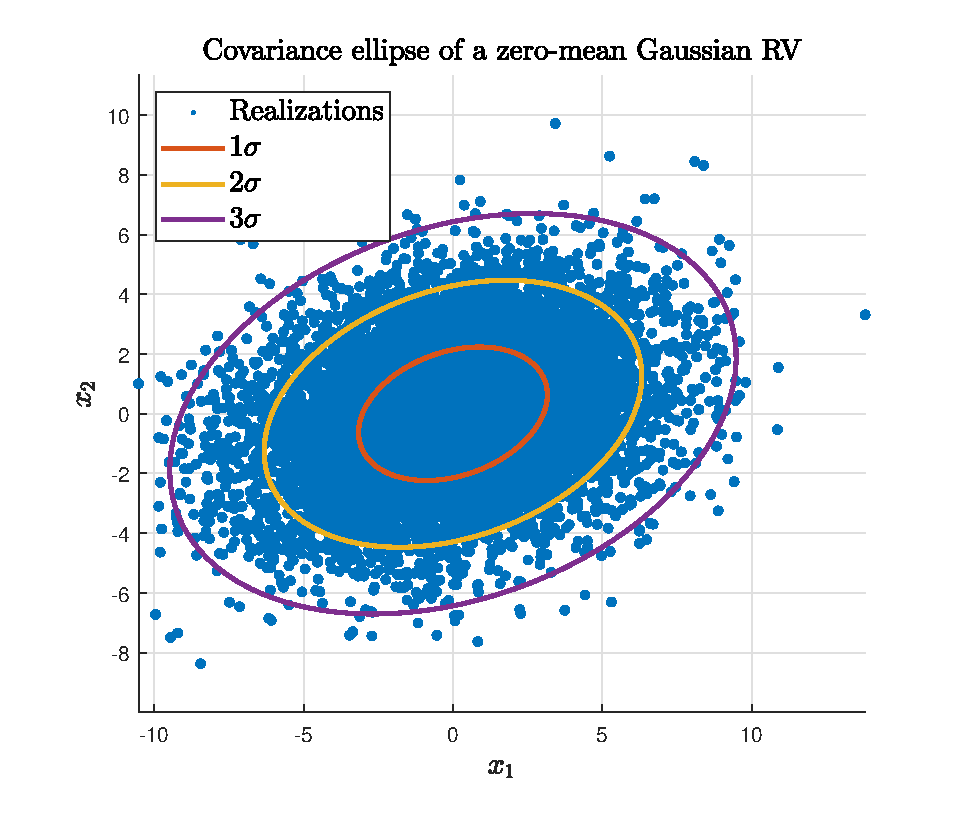
\includegraphics[width=0.8\textwidth]{figs/Covariance_ellipses_example.eps}    
    \caption{Covariance ellipses (actually, standard deviation ellipses) around $N=10^{4}$ samples.}
    \label{fig:Example covariance ellipses}
\end{figure}



\end{appendices}


% Add bib
\printbibliography


% Add indices
\addcontentsline{toc}{chapter}{Indices}
\printindex

\end{document}
